\section{General Linear Model (GLM) Results}
\subsection{Face Type Contrasts}
\begin{figure}[H]
    \centering
      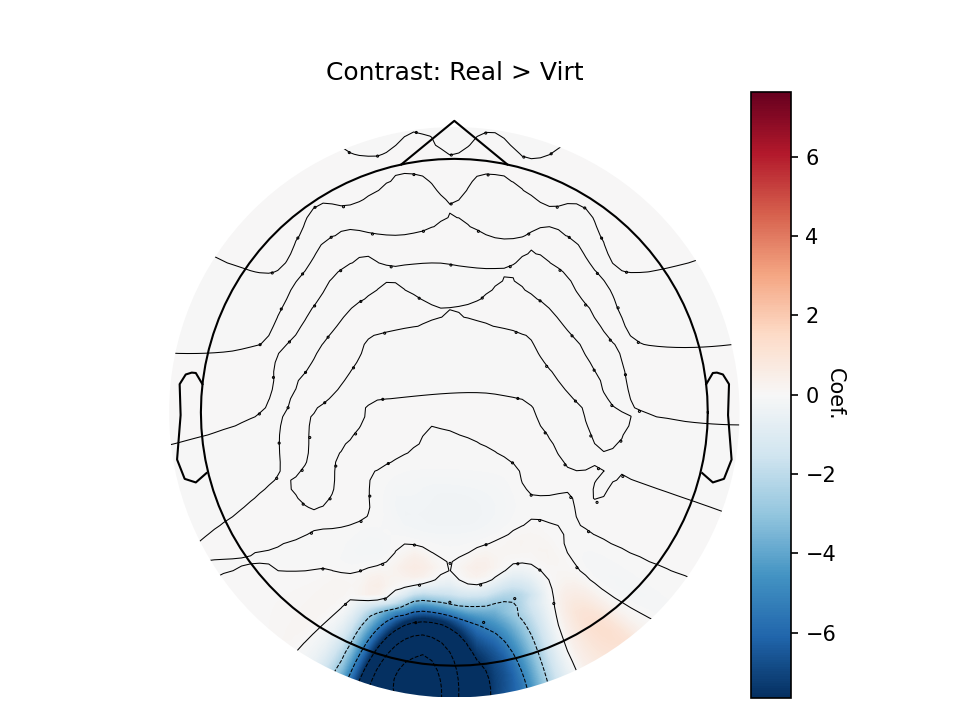
\includegraphics[width=0.85\textwidth]{C:/Users/super/OneDrive - Ontario Tech University/fNIRS_Emotions/plots/glm/contrasts/differences/Contrast_Real-Virt.png}
      \caption[GLM: Real vs. Virtual Faces]{GLM contrast between real and virtual conditions which shows the differences in activation between the two conditions.
      Red signifies that condition 1 (real faces) has more activation in that area than condition 2 (virtual faces), while blue signifies that condition 2 (virtual faces) has more activation than condition 1 (real faces).
      The color bar on the right shows the coefficient of the contrast, which indicates the strength of the difference in activation between the two conditions.}
      \label{fig:glm_real_vs_virtual}
\end{figure}

The main effect of real versus virtual faces (as shown in \ref{fig:glm_real_vs_virtual}) for the GLM revealed a significant difference in activation between real and virtual faces, with the left occipital channel showing greater activation for virtual faces compared to real faces.

\subsection{Emotion Contrasts}
\begin{figure}[H]
    \centering
    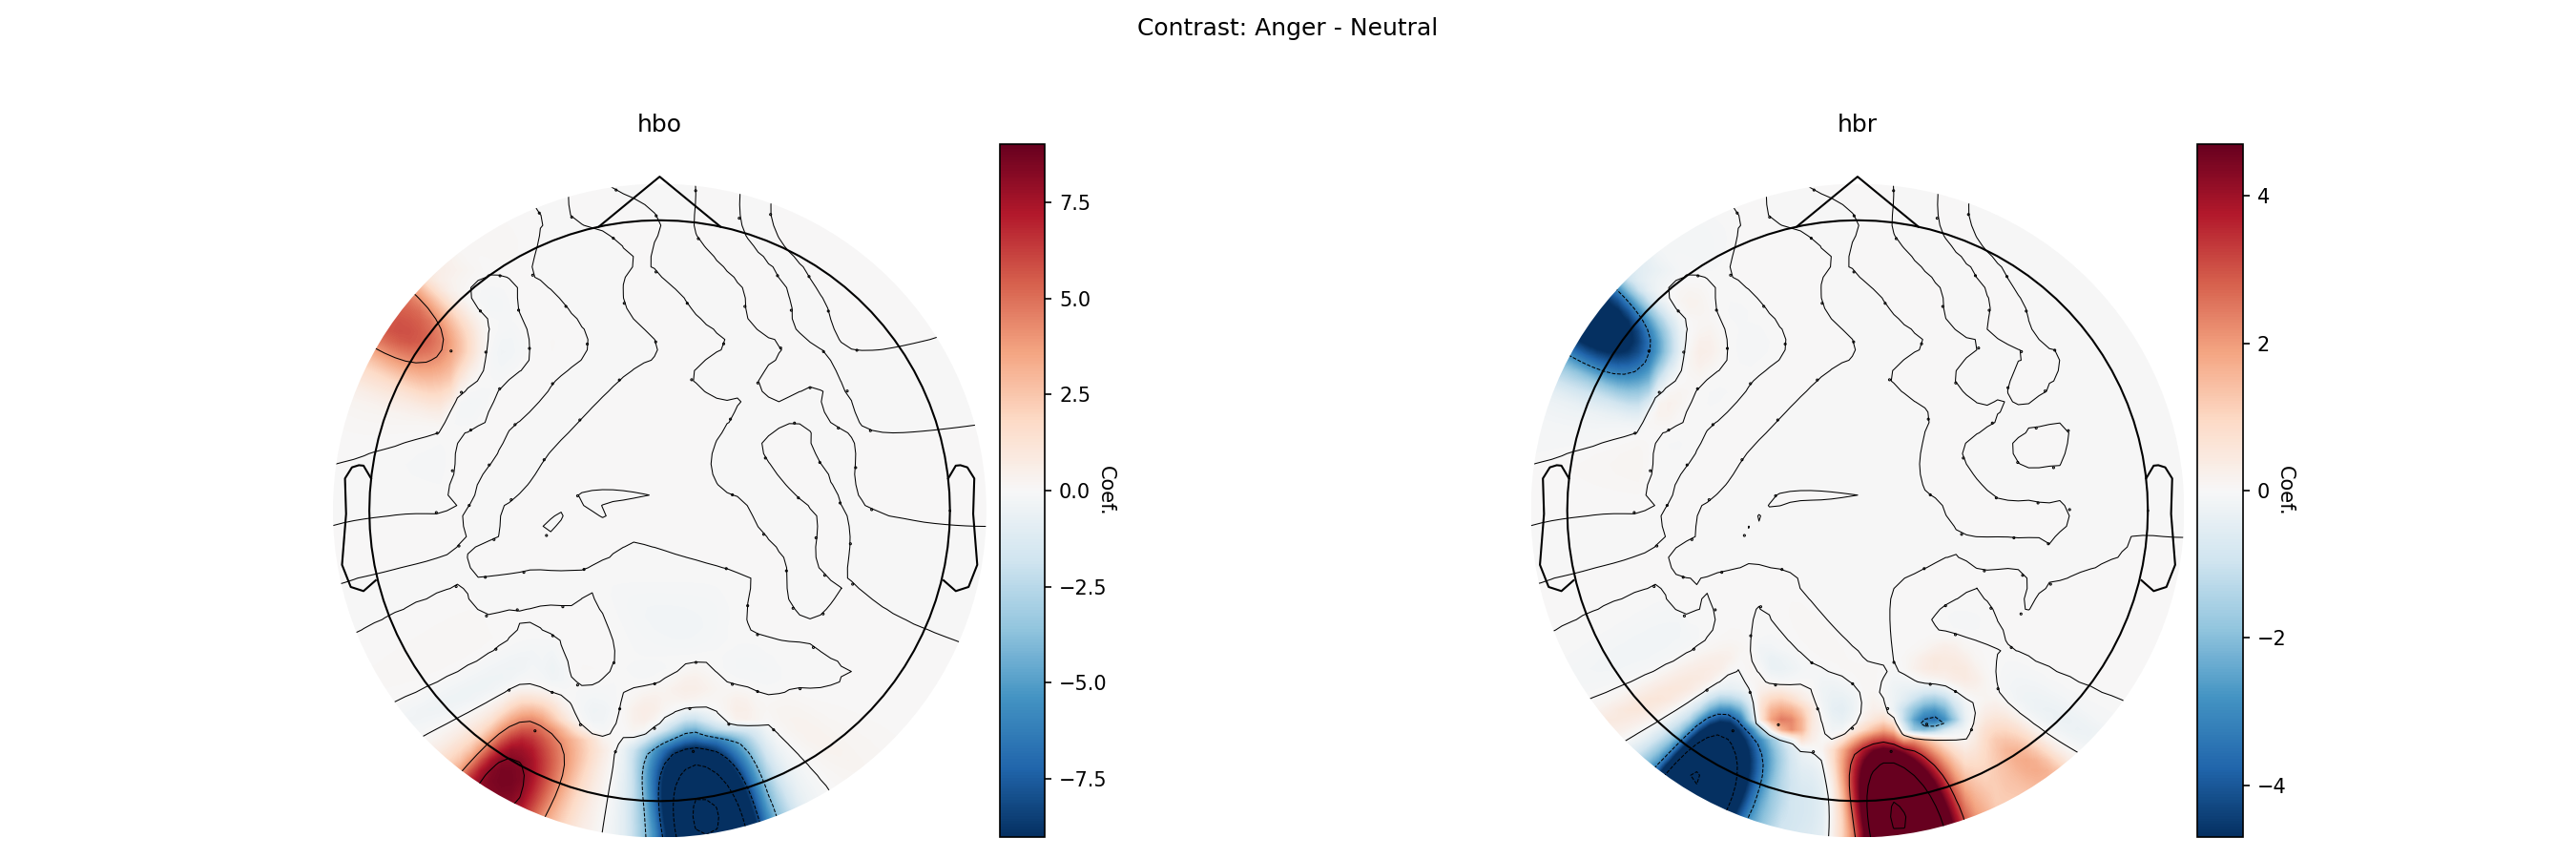
\includegraphics[width=0.45\textwidth]{C:/Users/super/OneDrive - Ontario Tech University/fNIRS_Emotions/plots/glm/contrasts/differences_neutral/Contrast_Anger-Neutral.png}
    
\includegraphics[width=0.45\textwidth]{C:/Users/super/OneDrive - Ontario Tech University/fNIRS_Emotions/plots/glm/contrasts/differences_neutral/Contrast_Fear-Neutral.png}
    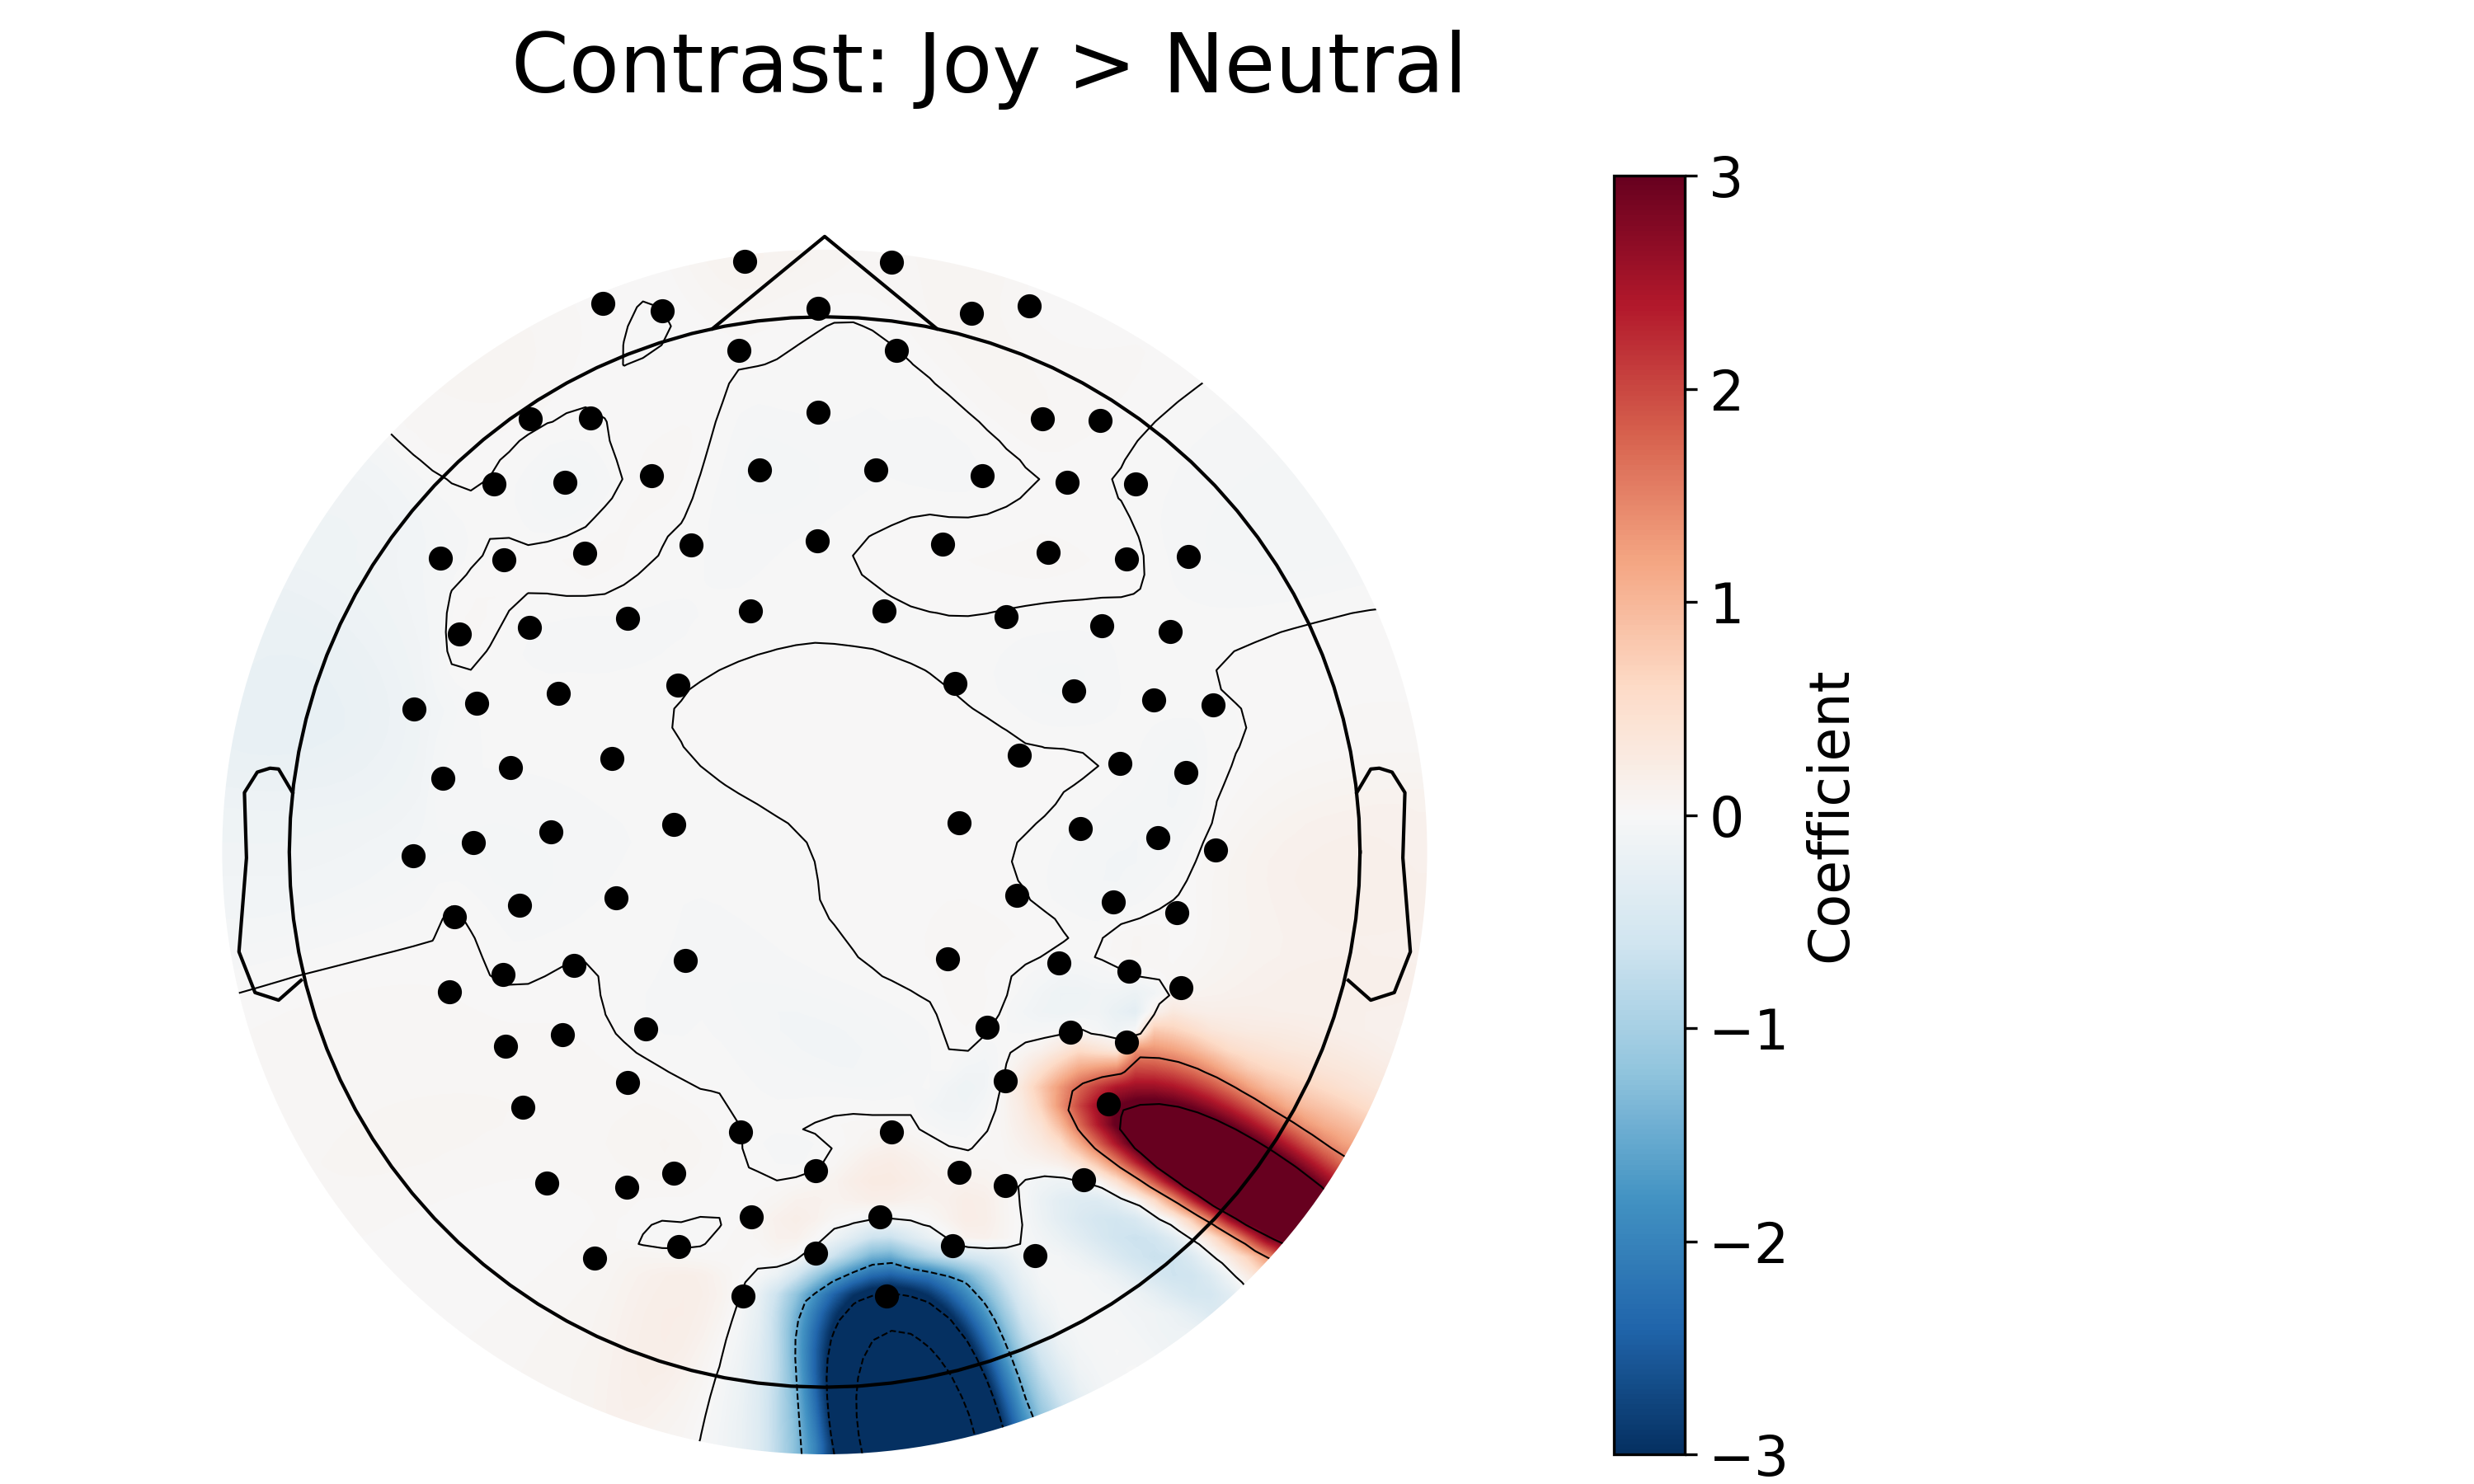
\includegraphics[width=0.45\textwidth]{C:/Users/super/OneDrive - Ontario Tech University/fNIRS_Emotions/plots/glm/contrasts/differences_neutral/Contrast_Joy-Neutral.png}
    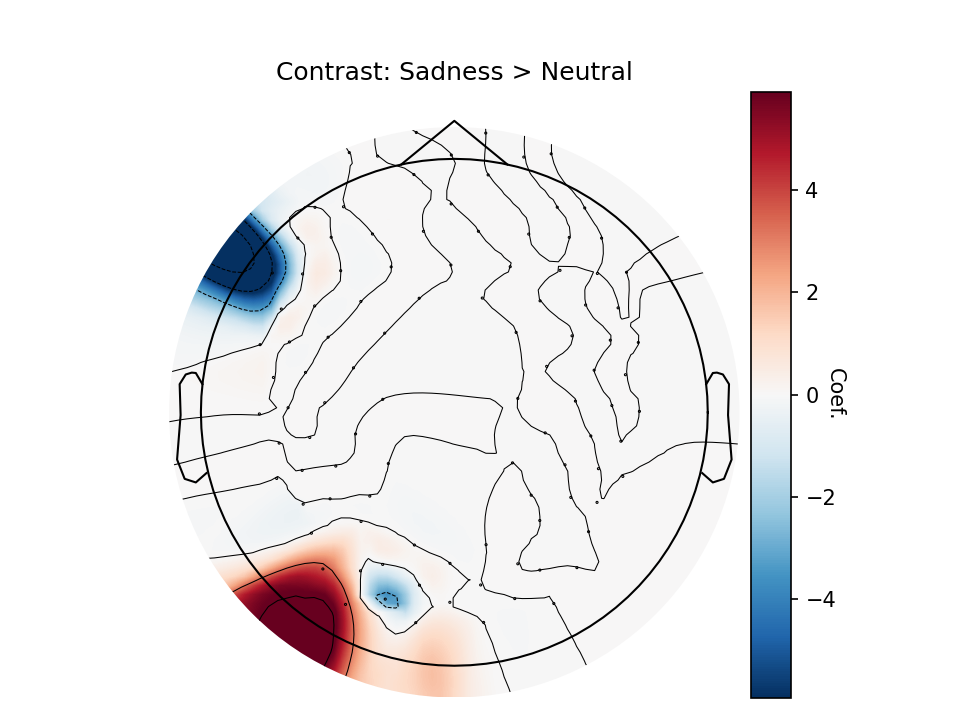
\includegraphics[width=0.45\textwidth]{C:/Users/super/OneDrive - Ontario Tech University/fNIRS_Emotions/plots/glm/contrasts/differences_neutral/Contrast_Sadness-Neutral.png}
    \caption[GLM: Emotion vs. Neutral]{GLM results for the contrast between different emotions and neutral condition.
    Same concept as explained in figure \ref{fig:glm_real_vs_virtual}. }
    \label{fig:glm_emotion_analysis_neutral}
\end{figure}

Against the Neutral emotion (as shown in \ref{fig:glm_emotion_analysis_neutral}), the emotion contrasts revealed significant differences in activation across several brain regions. 
Specifically, Anger and Fear elicited greater activation in the right occipital region compared to Neutral. 
Joy was associated with increased activation in the right parietal region and decreased activation in the right occipital region, while sadness showed reduced activation in the left frontal region relative to Neutral. 
These results indicate distinct neural activation patterns for each emotion when contrasted with the Neutral baseline.

\begin{figure}[H]
    \centering
      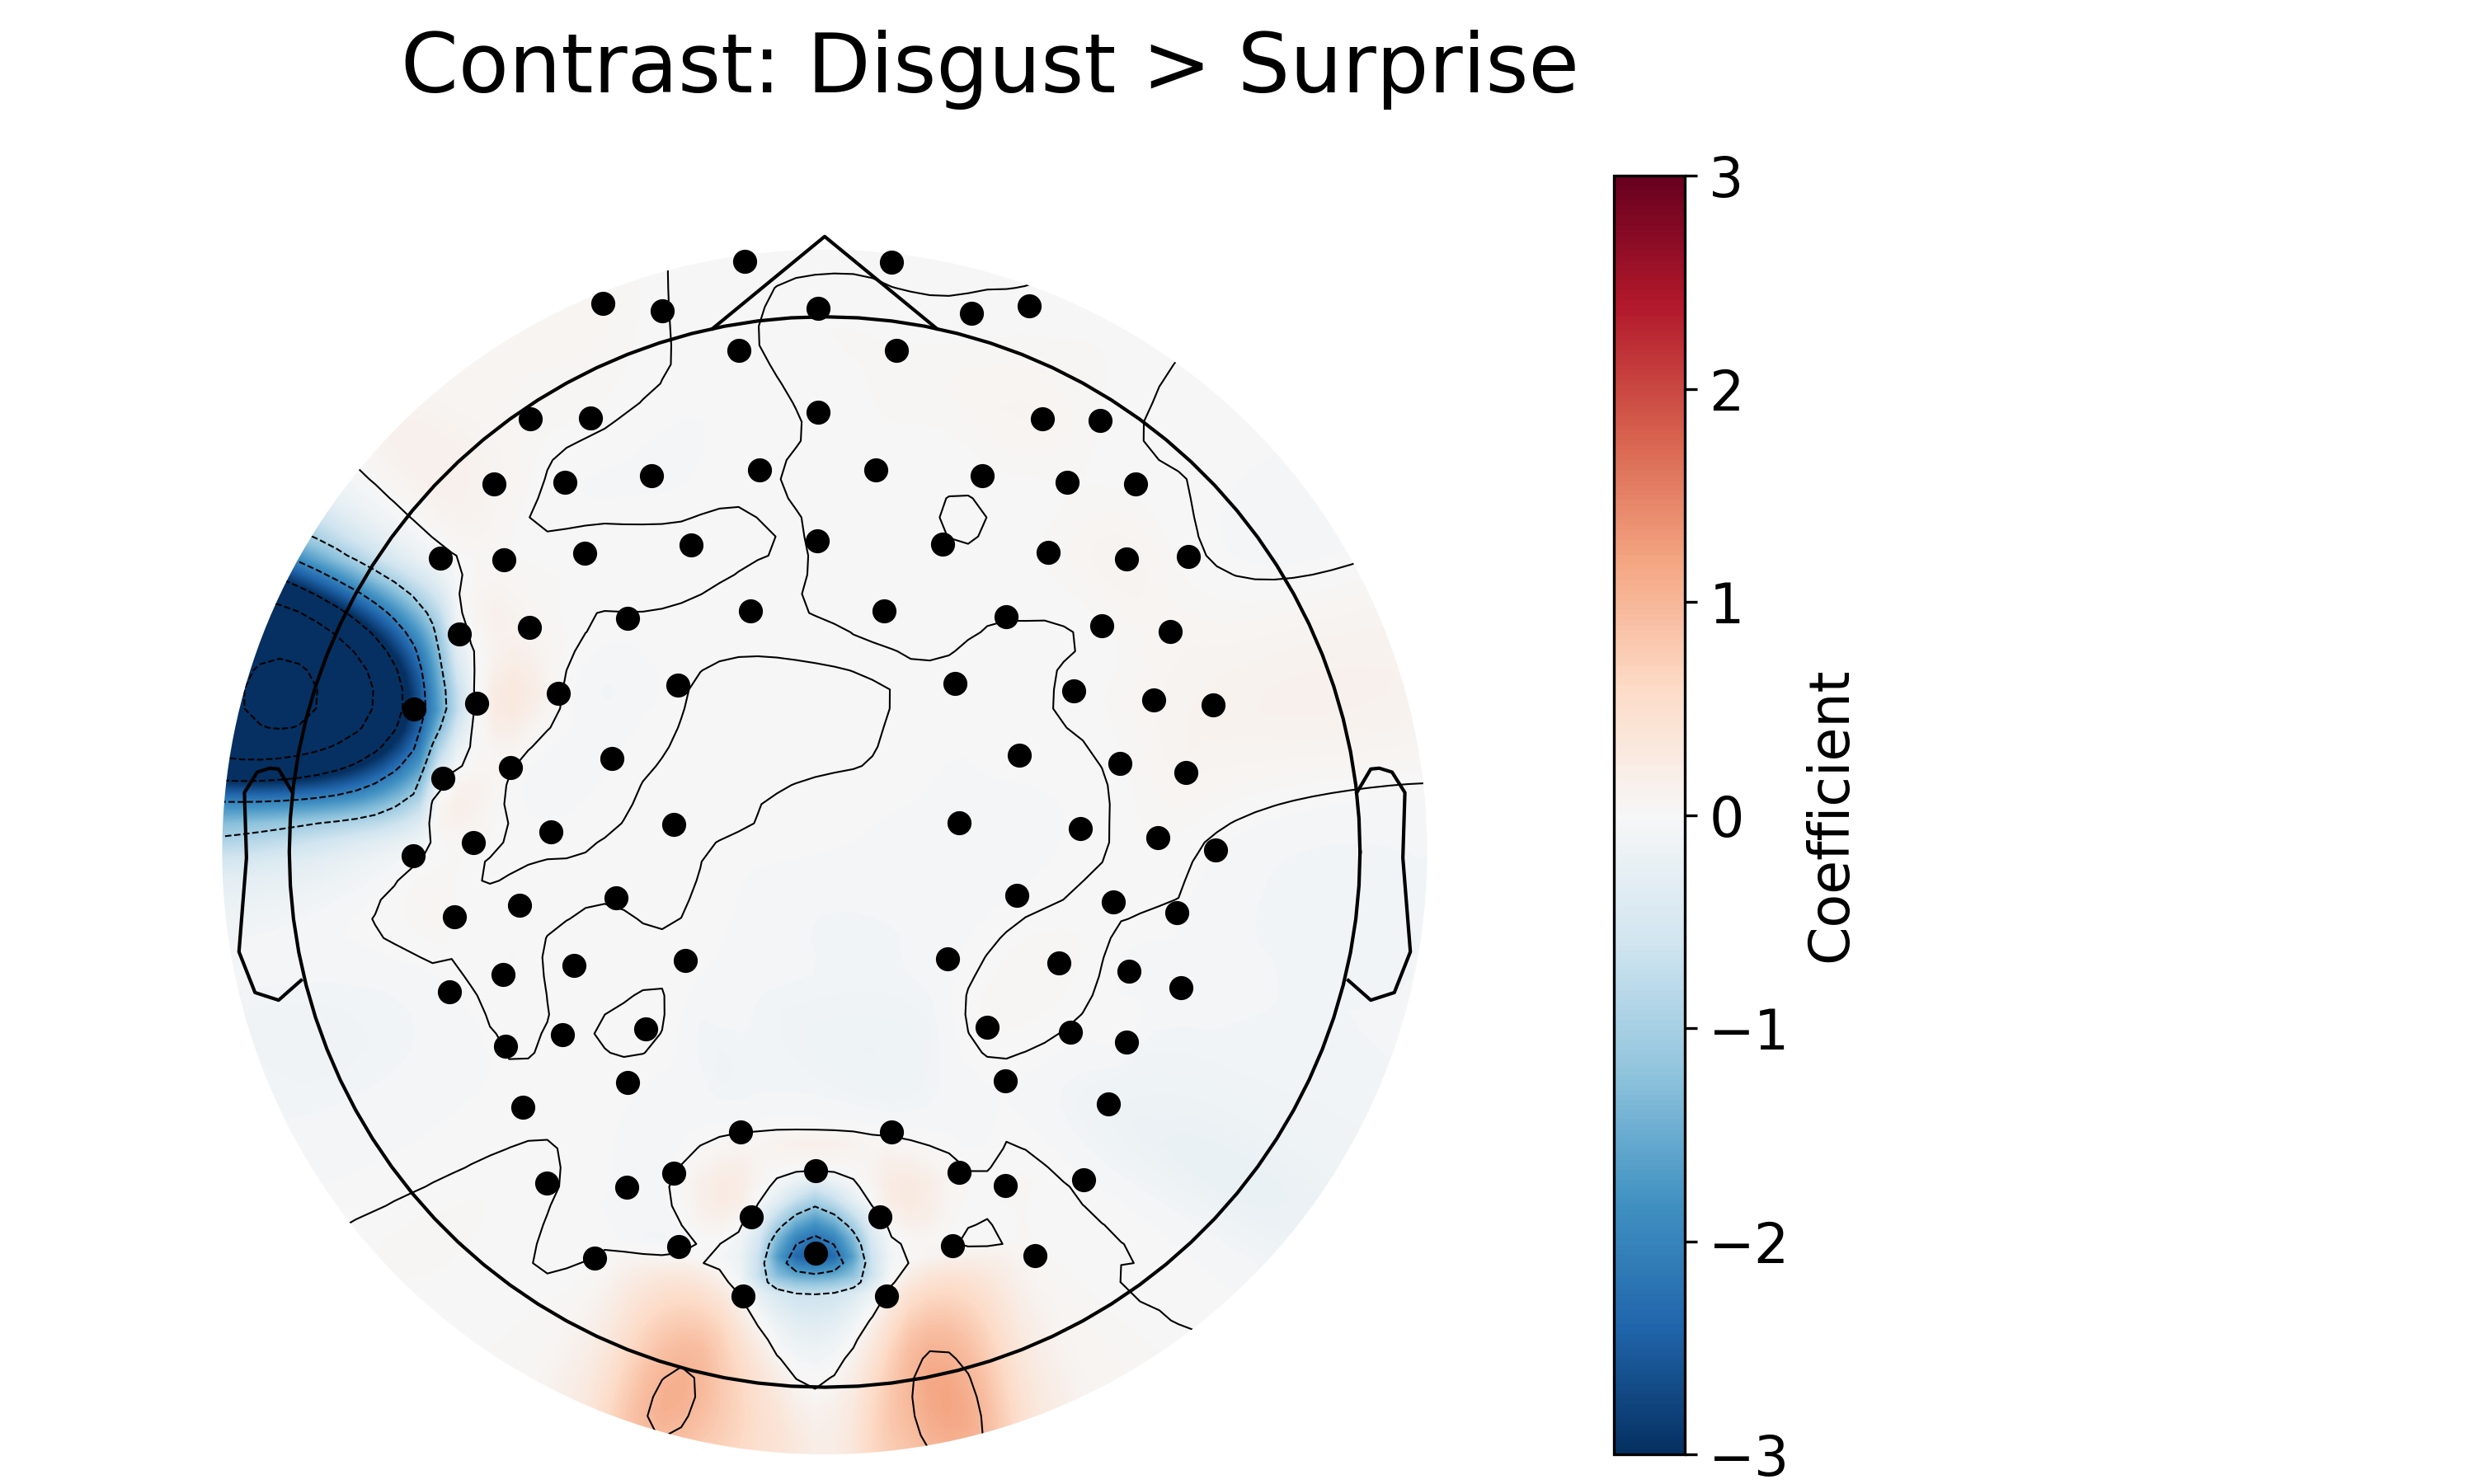
\includegraphics[width=0.45\textwidth]{C:/Users/super/OneDrive - Ontario Tech University/fNIRS_Emotions/plots/glm/contrasts/differences/Contrast_Disgust-Surprise.png}
      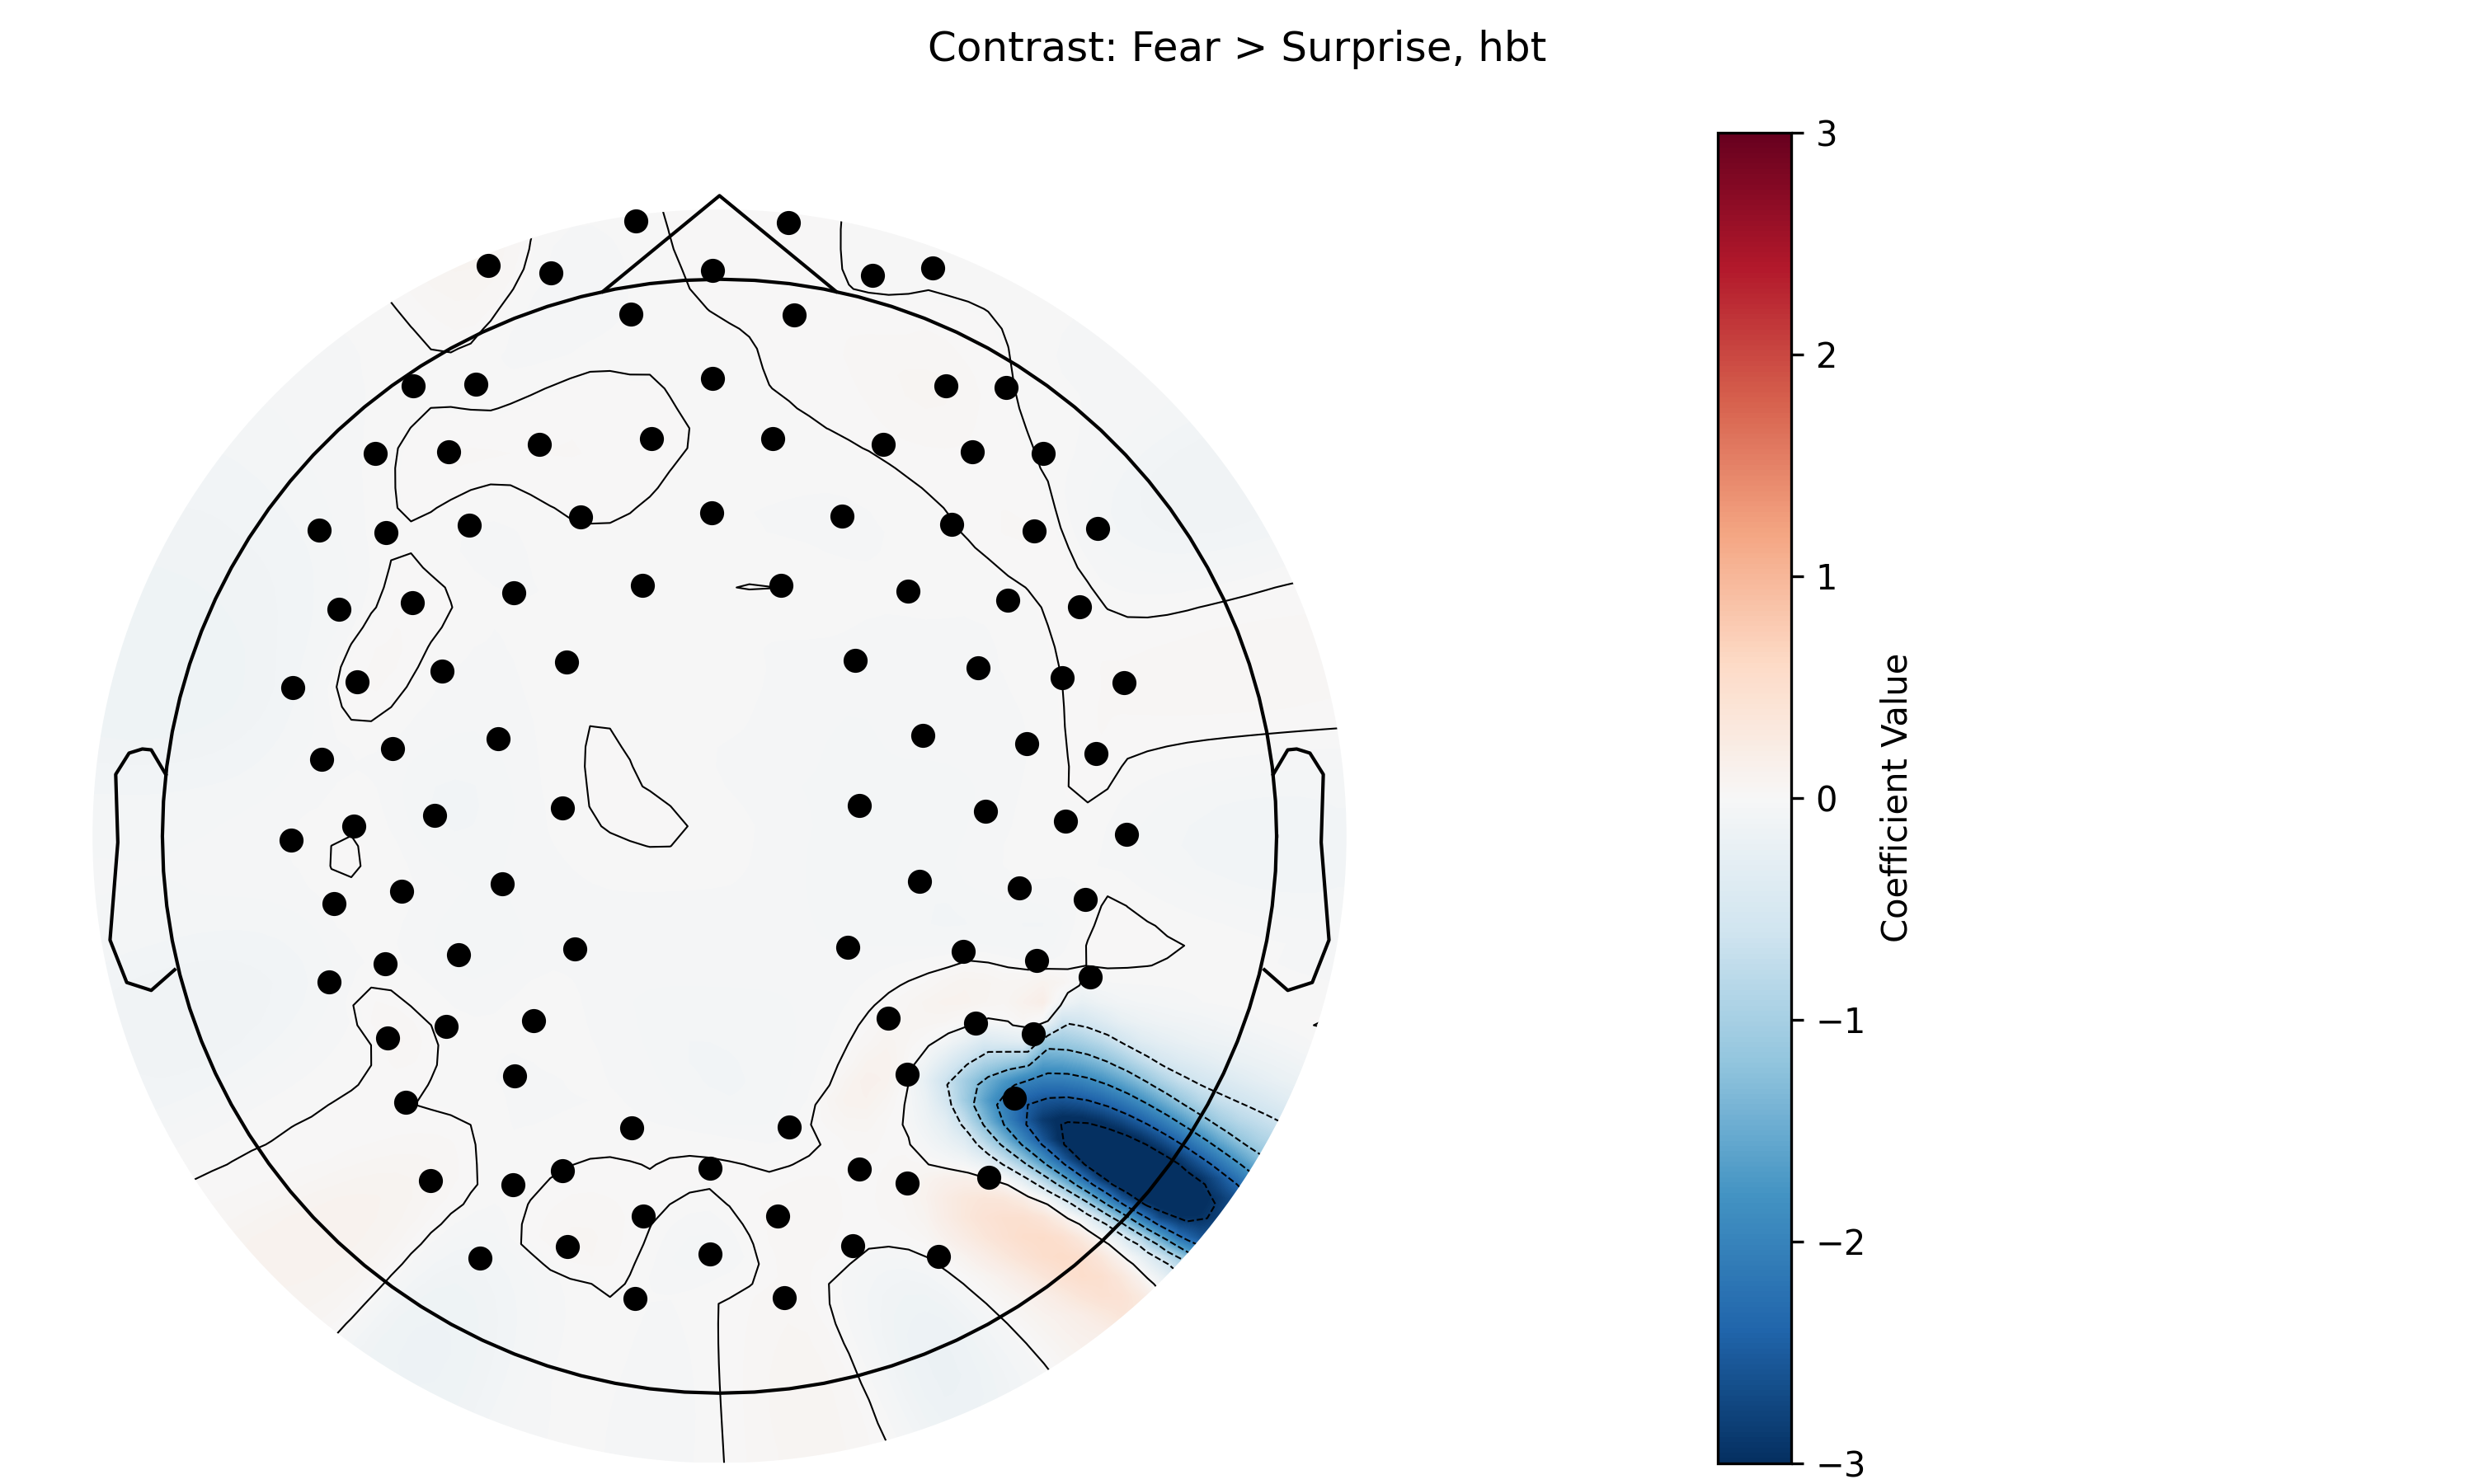
\includegraphics[width=0.45\textwidth]{C:/Users/super/OneDrive - Ontario Tech University/fNIRS_Emotions/plots/glm/contrasts/differences/Contrast_Fear-Surprise.png}
      
\includegraphics[width=0.45\textwidth]{C:/Users/super/OneDrive - Ontario Tech University/fNIRS_Emotions/plots/glm/contrasts/differences/Contrast_Joy-Surprise.png}
      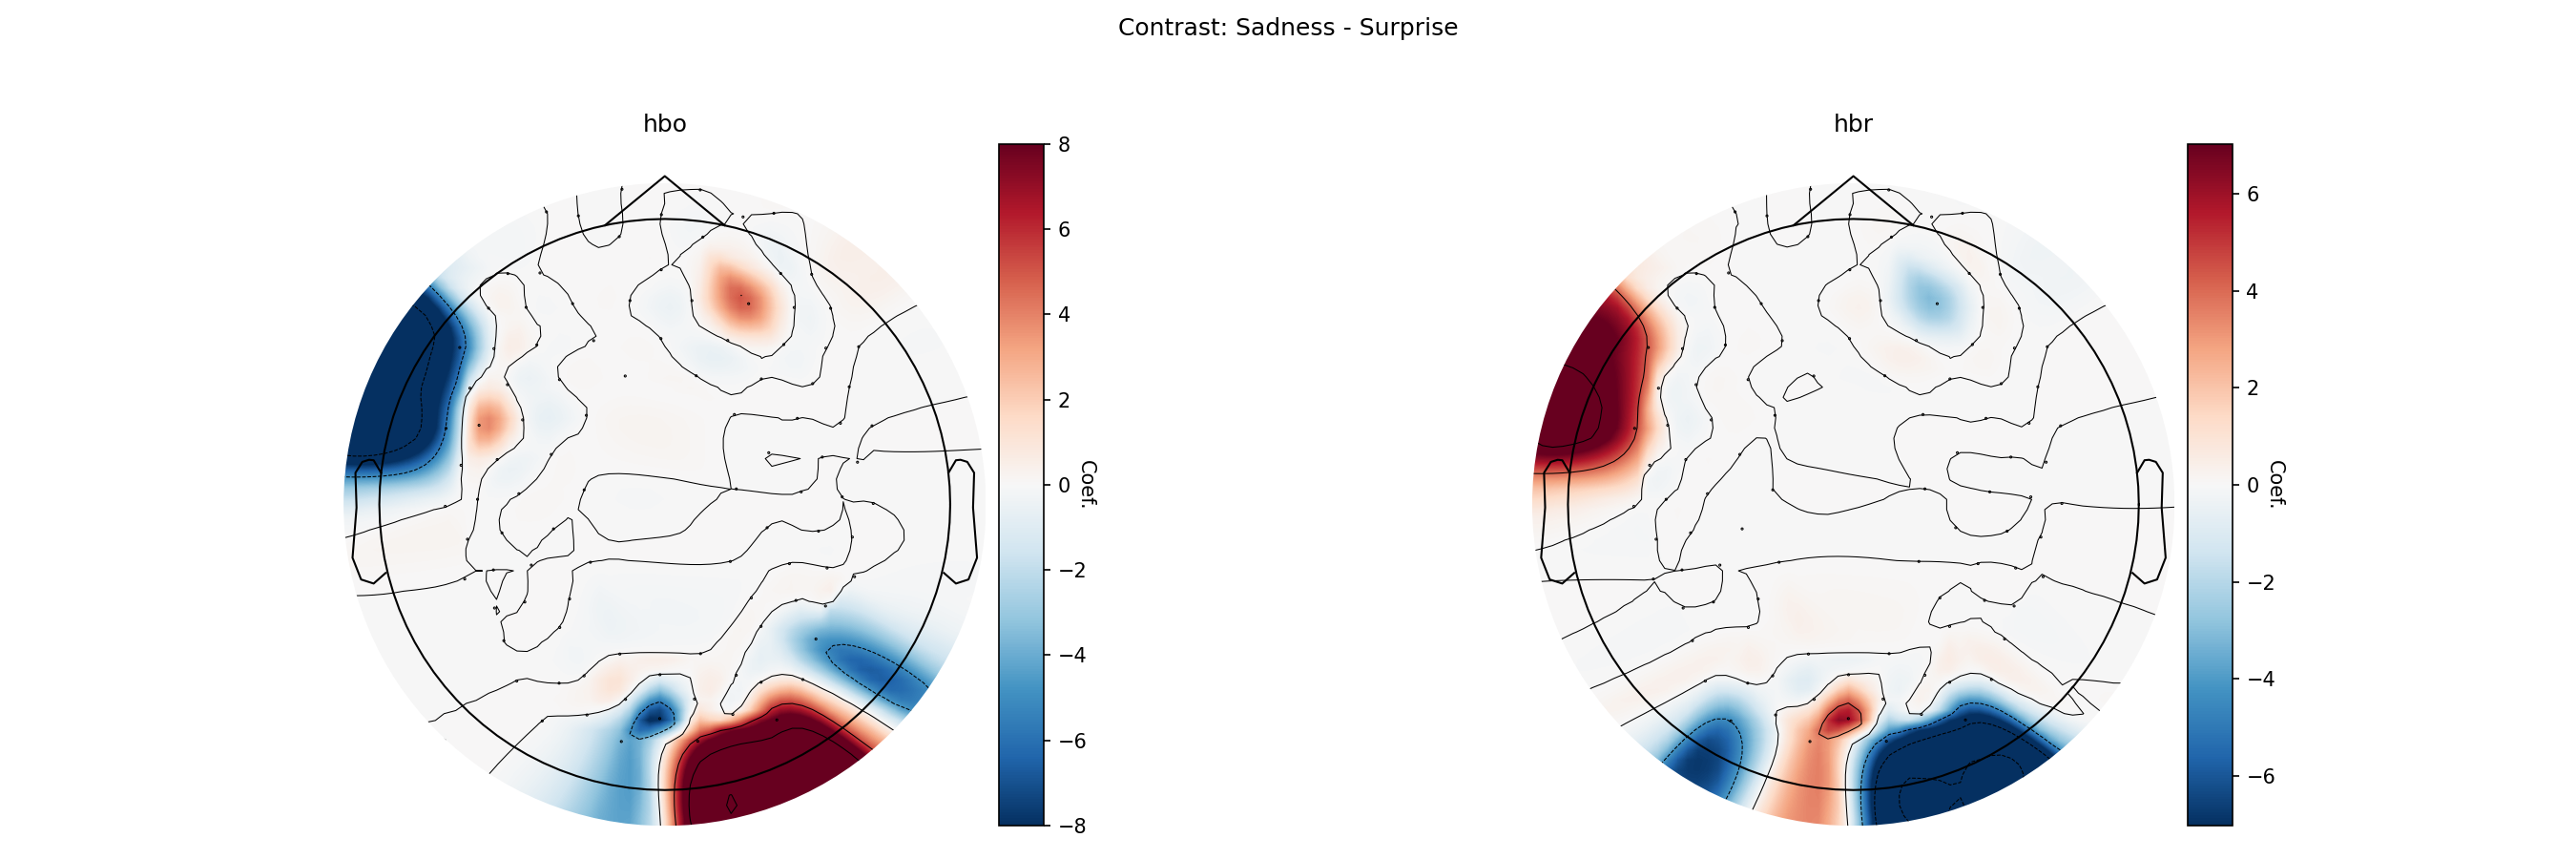
\includegraphics[width=0.45\textwidth]{C:/Users/super/OneDrive - Ontario Tech University/fNIRS_Emotions/plots/glm/contrasts/differences/Contrast_Sadness-Surprise.png}
      \caption[GLM: Emotion vs. Surprise]{GLM results for the contrast between different emotions and surprise condition.
      Same concept as explained in figure \ref{fig:glm_real_vs_virtual}. }
      \label{fig:glm_emotion_analysis_surprise}
\end{figure}

When comparing each emotion against Surprise (as shown in \ref{fig:glm_emotion_analysis_surprise}), significant differences in activation were observed across multiple brain regions. 
Disgust and Joy both showed decreased activation in the right occipital and left prefrontal regions relative to Surprise. 
Fear was associated with reduced activation in the right parietal region, while Sadness showed decreased activation in both the left frontal and right parietal regions. 
These findings suggest that each emotion, when contrasted with Surprise, elicits distinct neural activation patterns all across the brain, rather than being limited to specific regions.

\begin{figure}[H]
    \centering
      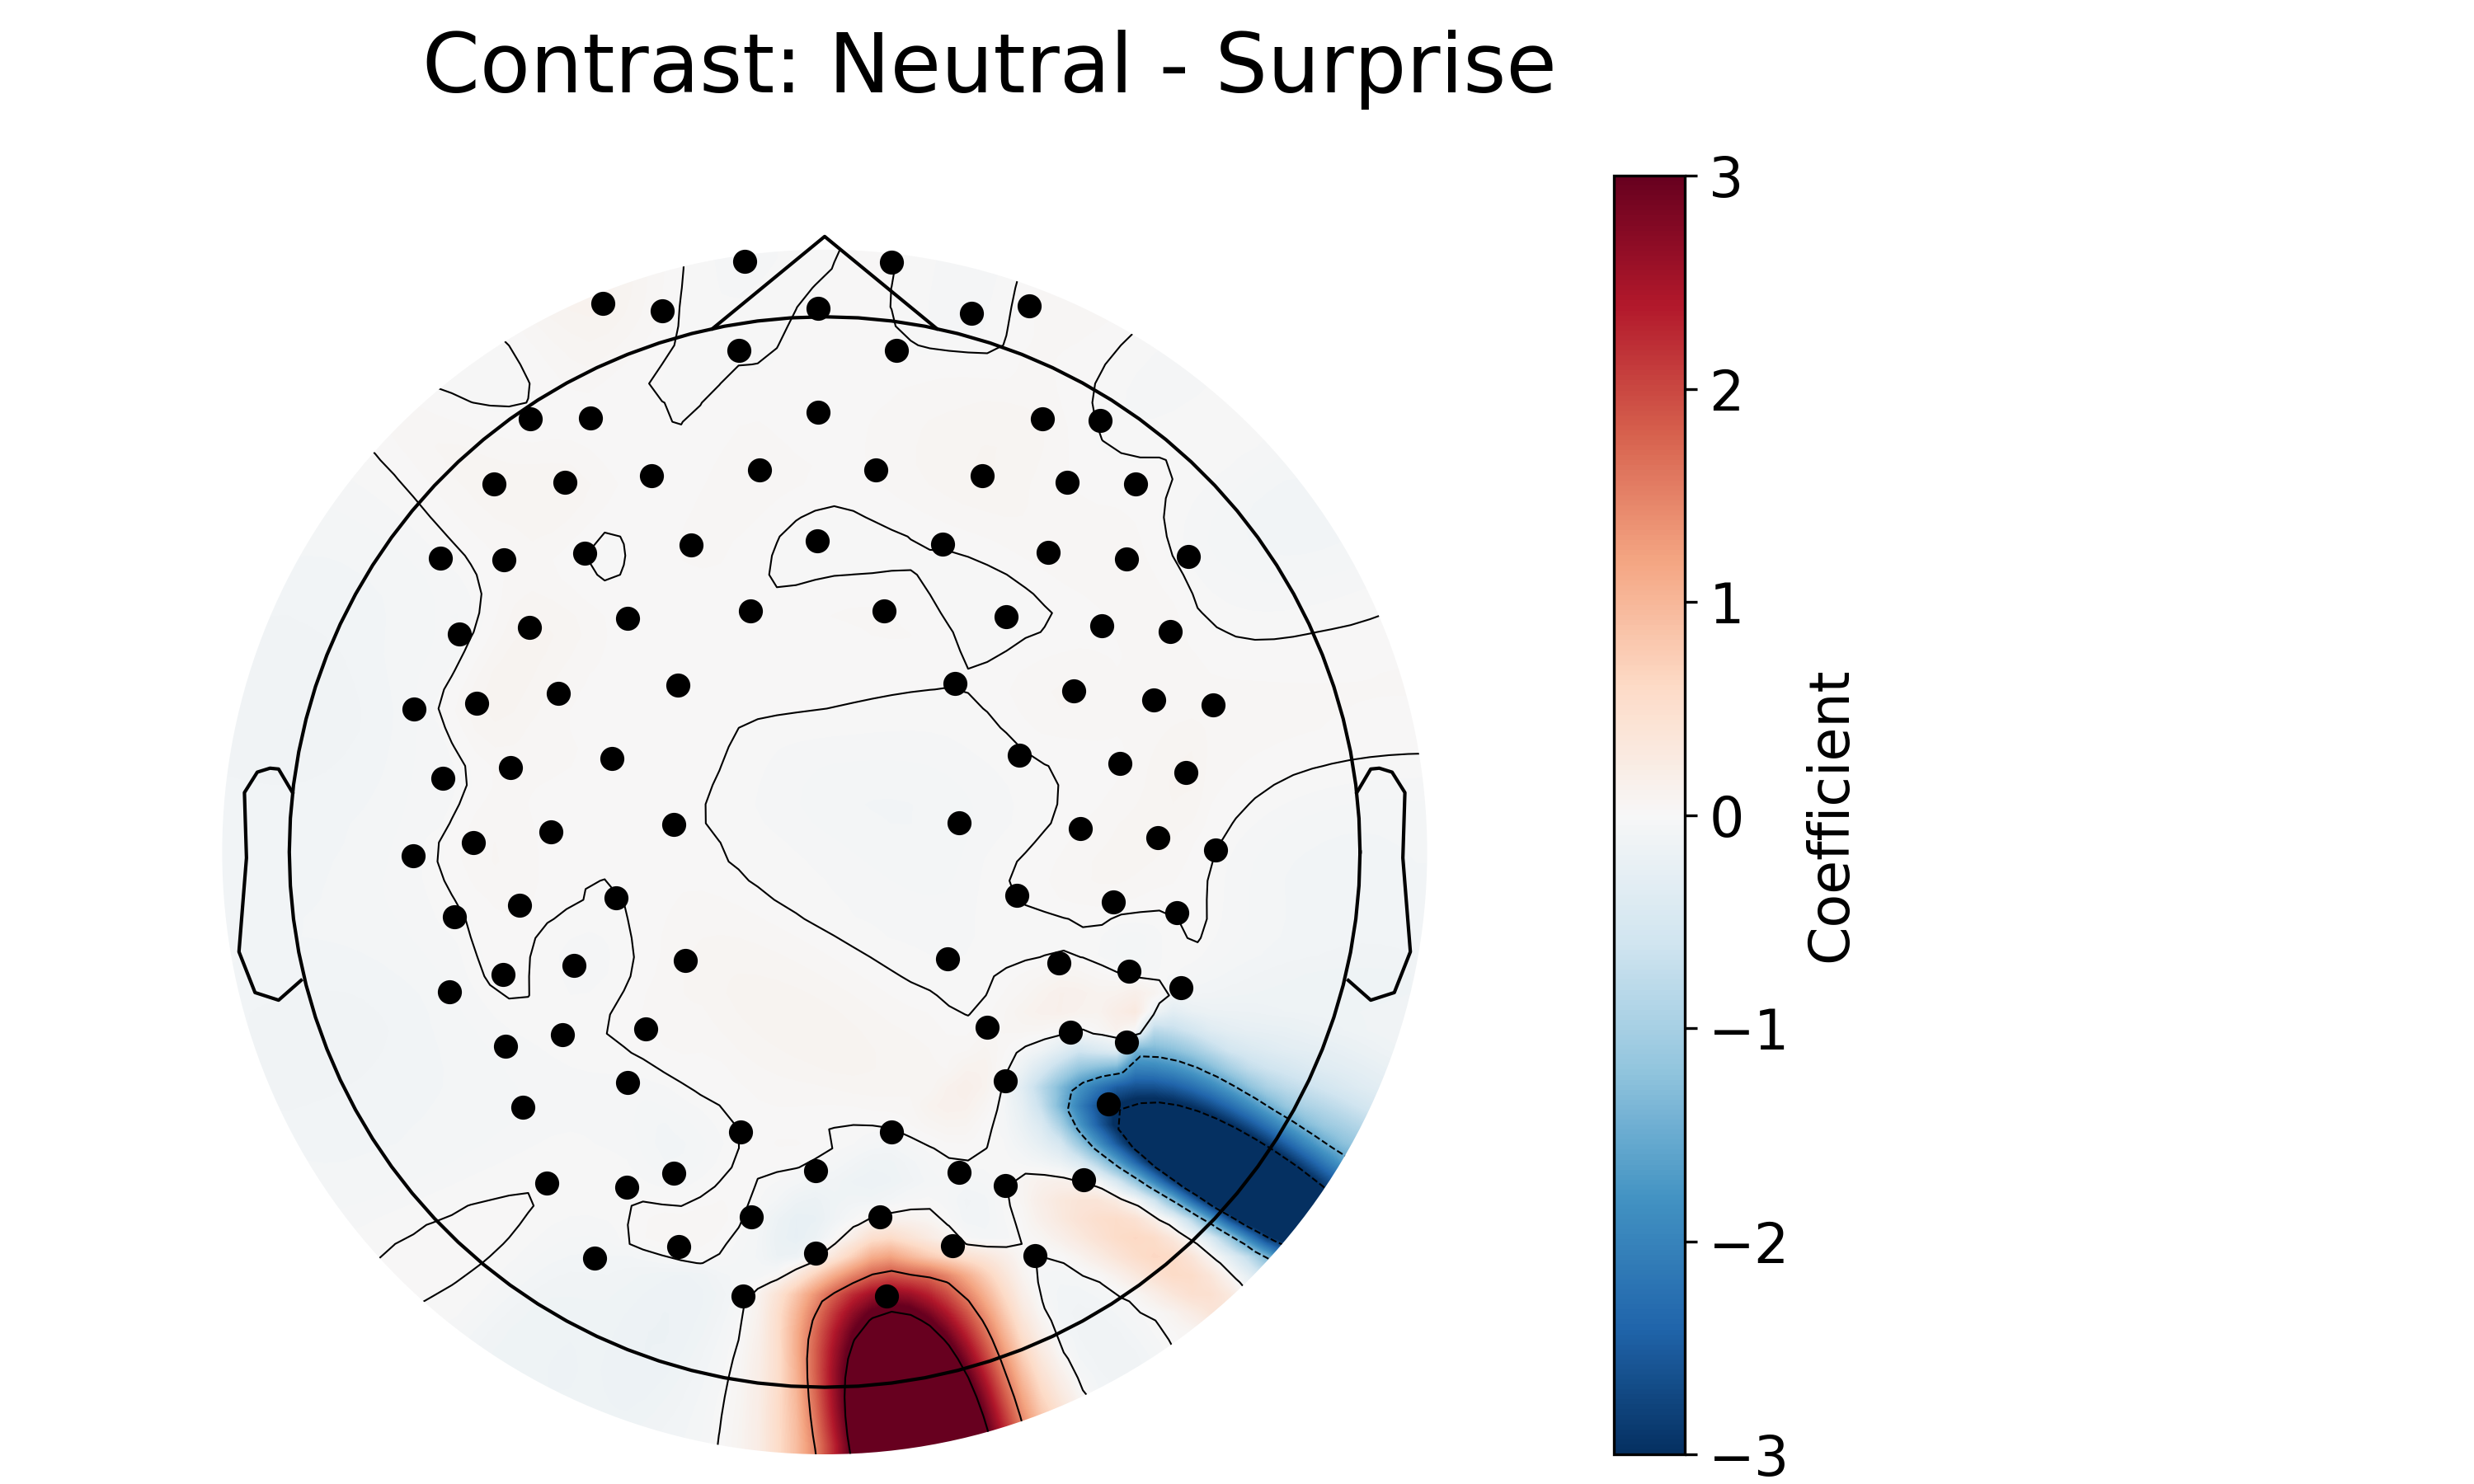
\includegraphics[width=0.85\textwidth]{C:/Users/super/OneDrive - Ontario Tech University/fNIRS_Emotions/plots/glm/contrasts/differences_neutral/Contrast_Neutral-Surprise.png}
      \caption[GLM: Neutral vs. Surprise]{GLM results for the contrast between neutral and surprise condition.
      Same concept as explained in figure \ref{fig:glm_real_vs_virtual}. }
      \label{fig:glm_neutral_vs_surprise}
\end{figure}

The Neutral $>$ Surprise comparison (as shown in \ref{fig:glm_neutral_vs_surprise}) revealed significant differences in the right parietal and right occipital regions. 
The right parietal region showed decreased activation (more activation for Surprise) while the right occipital region showed increased activation (more activation for neutral).
Both Neutral and Surprise conditions elicit greater activation when compared to the other emotions, but when compared to each other, one emotion is not more activated than the other.
This indicates that the neural response to Neutral and Surprise conditions is distinct, with each condition eliciting different activation patterns in specific brain regions.
Note that all combinations of emotion contrasts were performed, no other significant differences were found between any other emotions than the ones shown in this section.

\subsection{Face Type \texorpdfstring{$\times$}{x} Emotion Contrasts}
\begin{figure}[H]
  \centering
  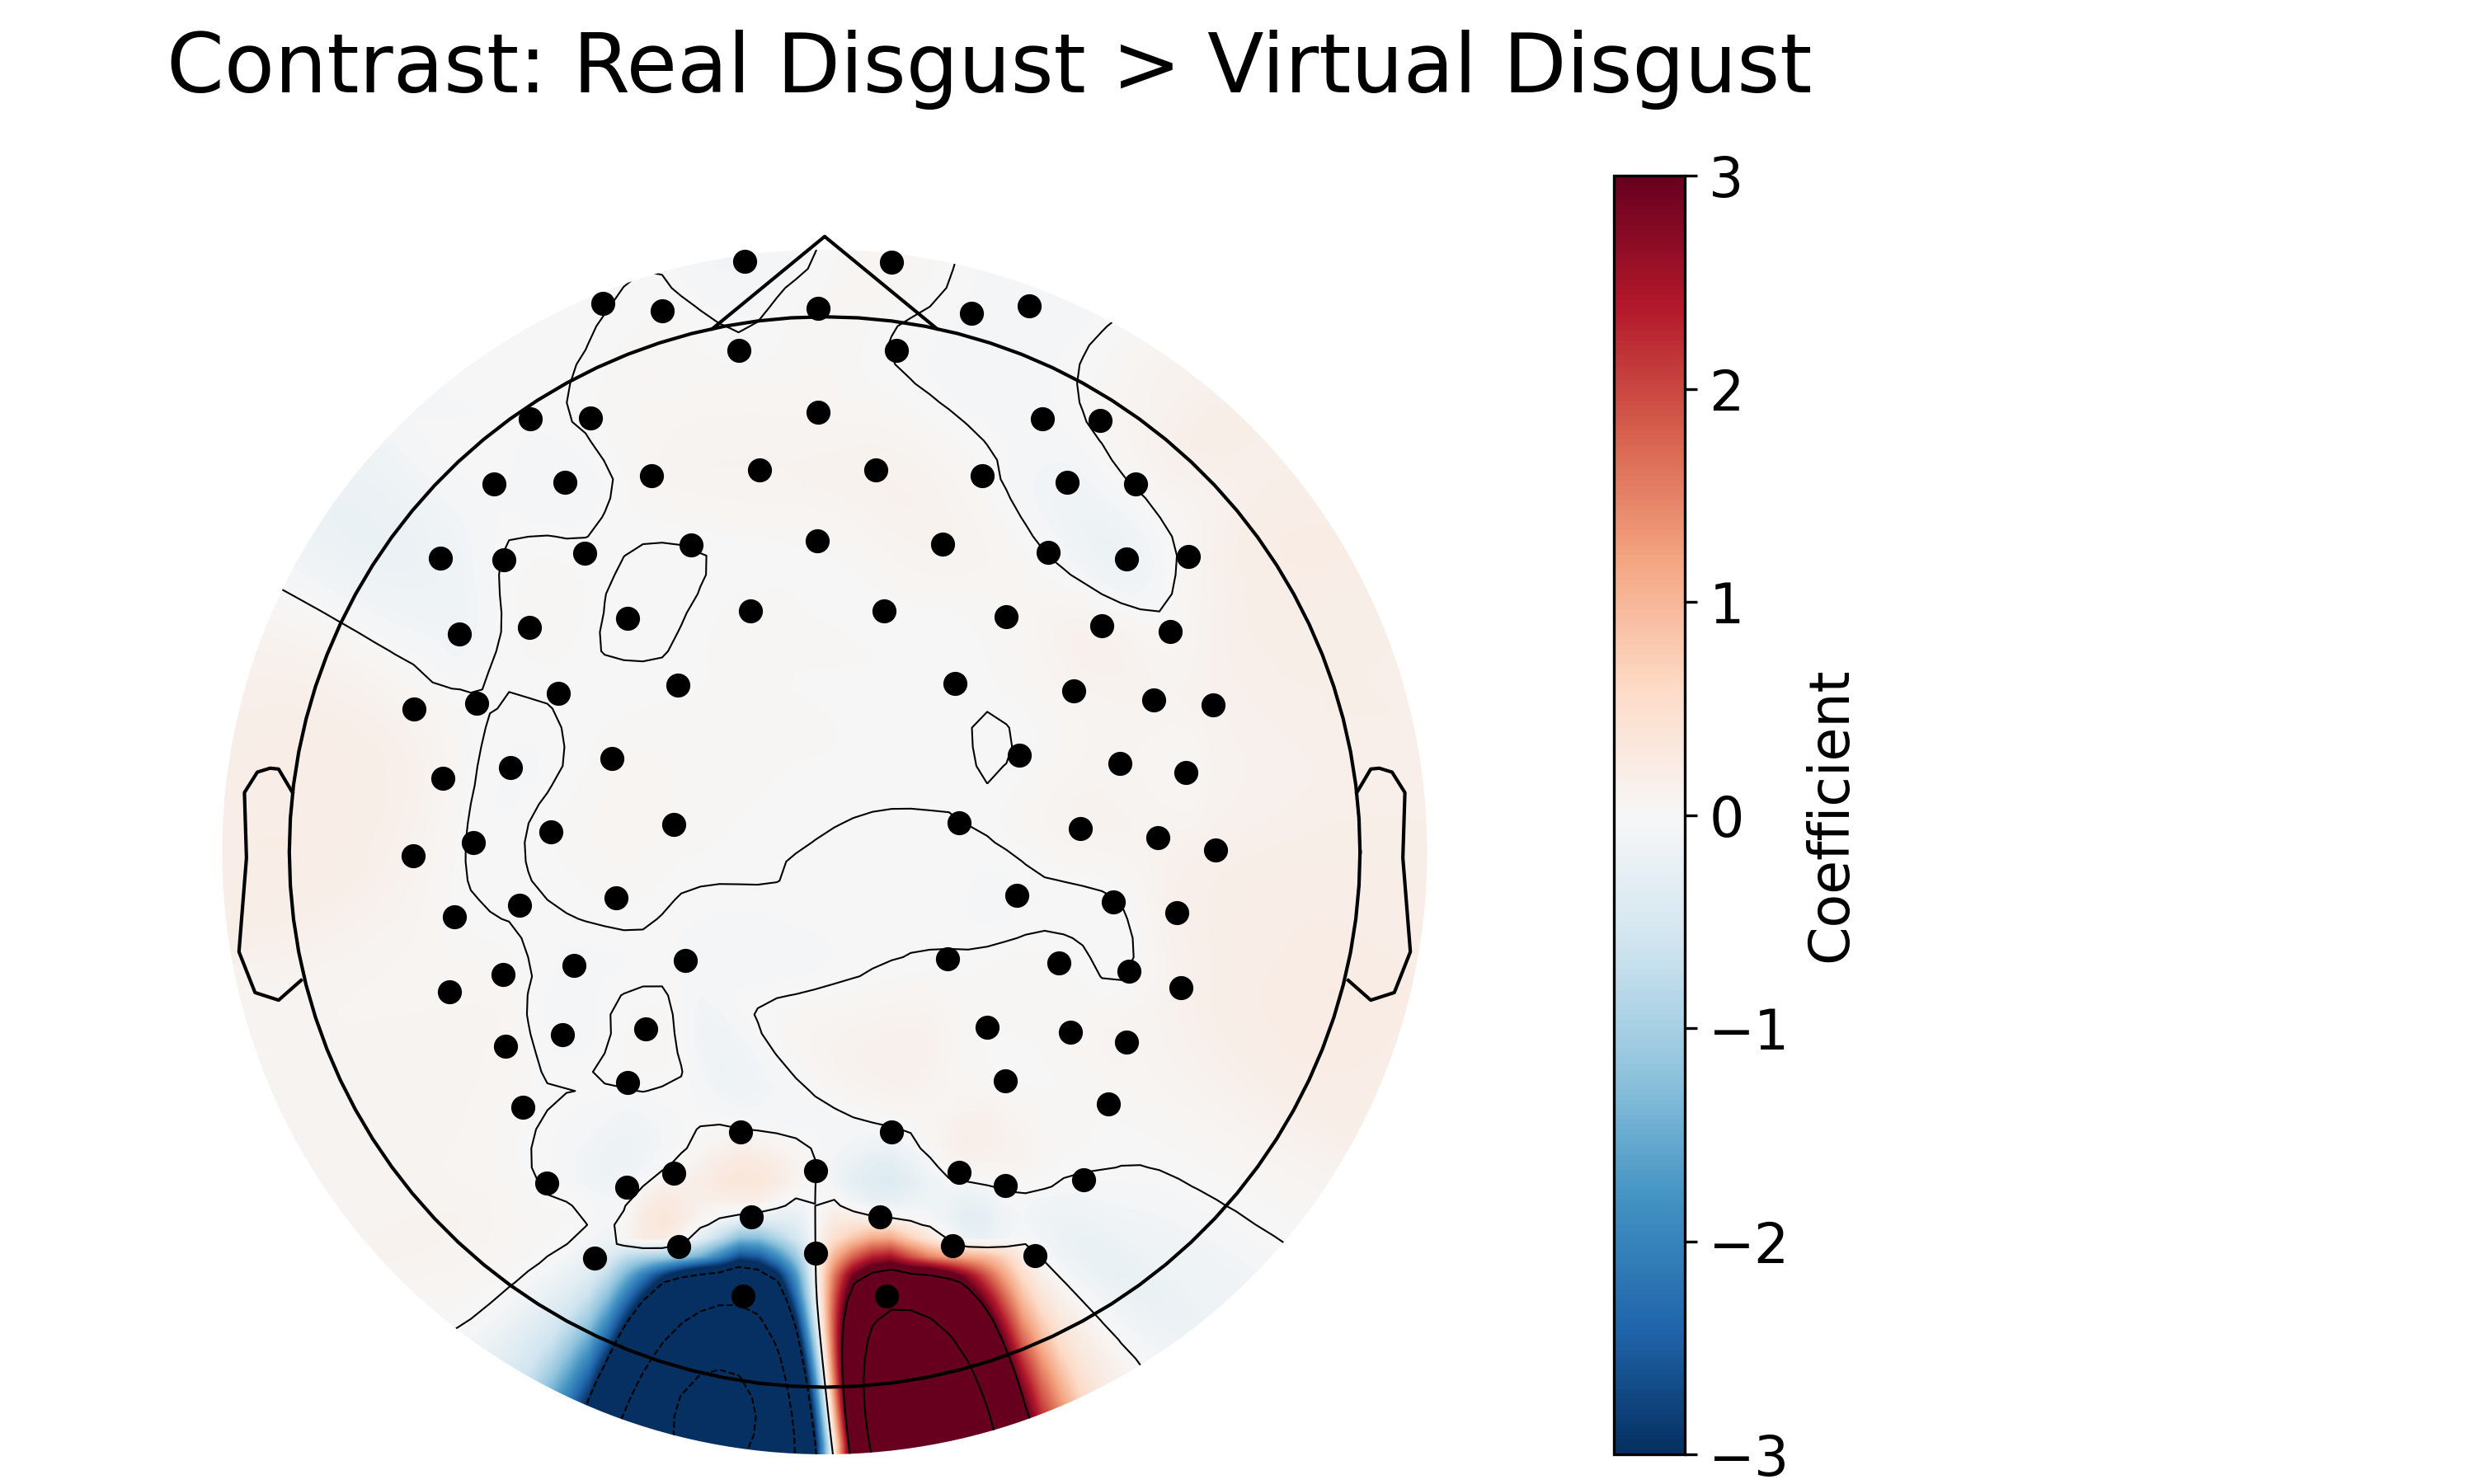
\includegraphics[width=0.45\textwidth]{C:/Users/super/OneDrive - Ontario Tech University/fNIRS_Emotions/plots/glm/contrasts/differences/Contrast_Real_Disgust-Virt_Disgust.png}
  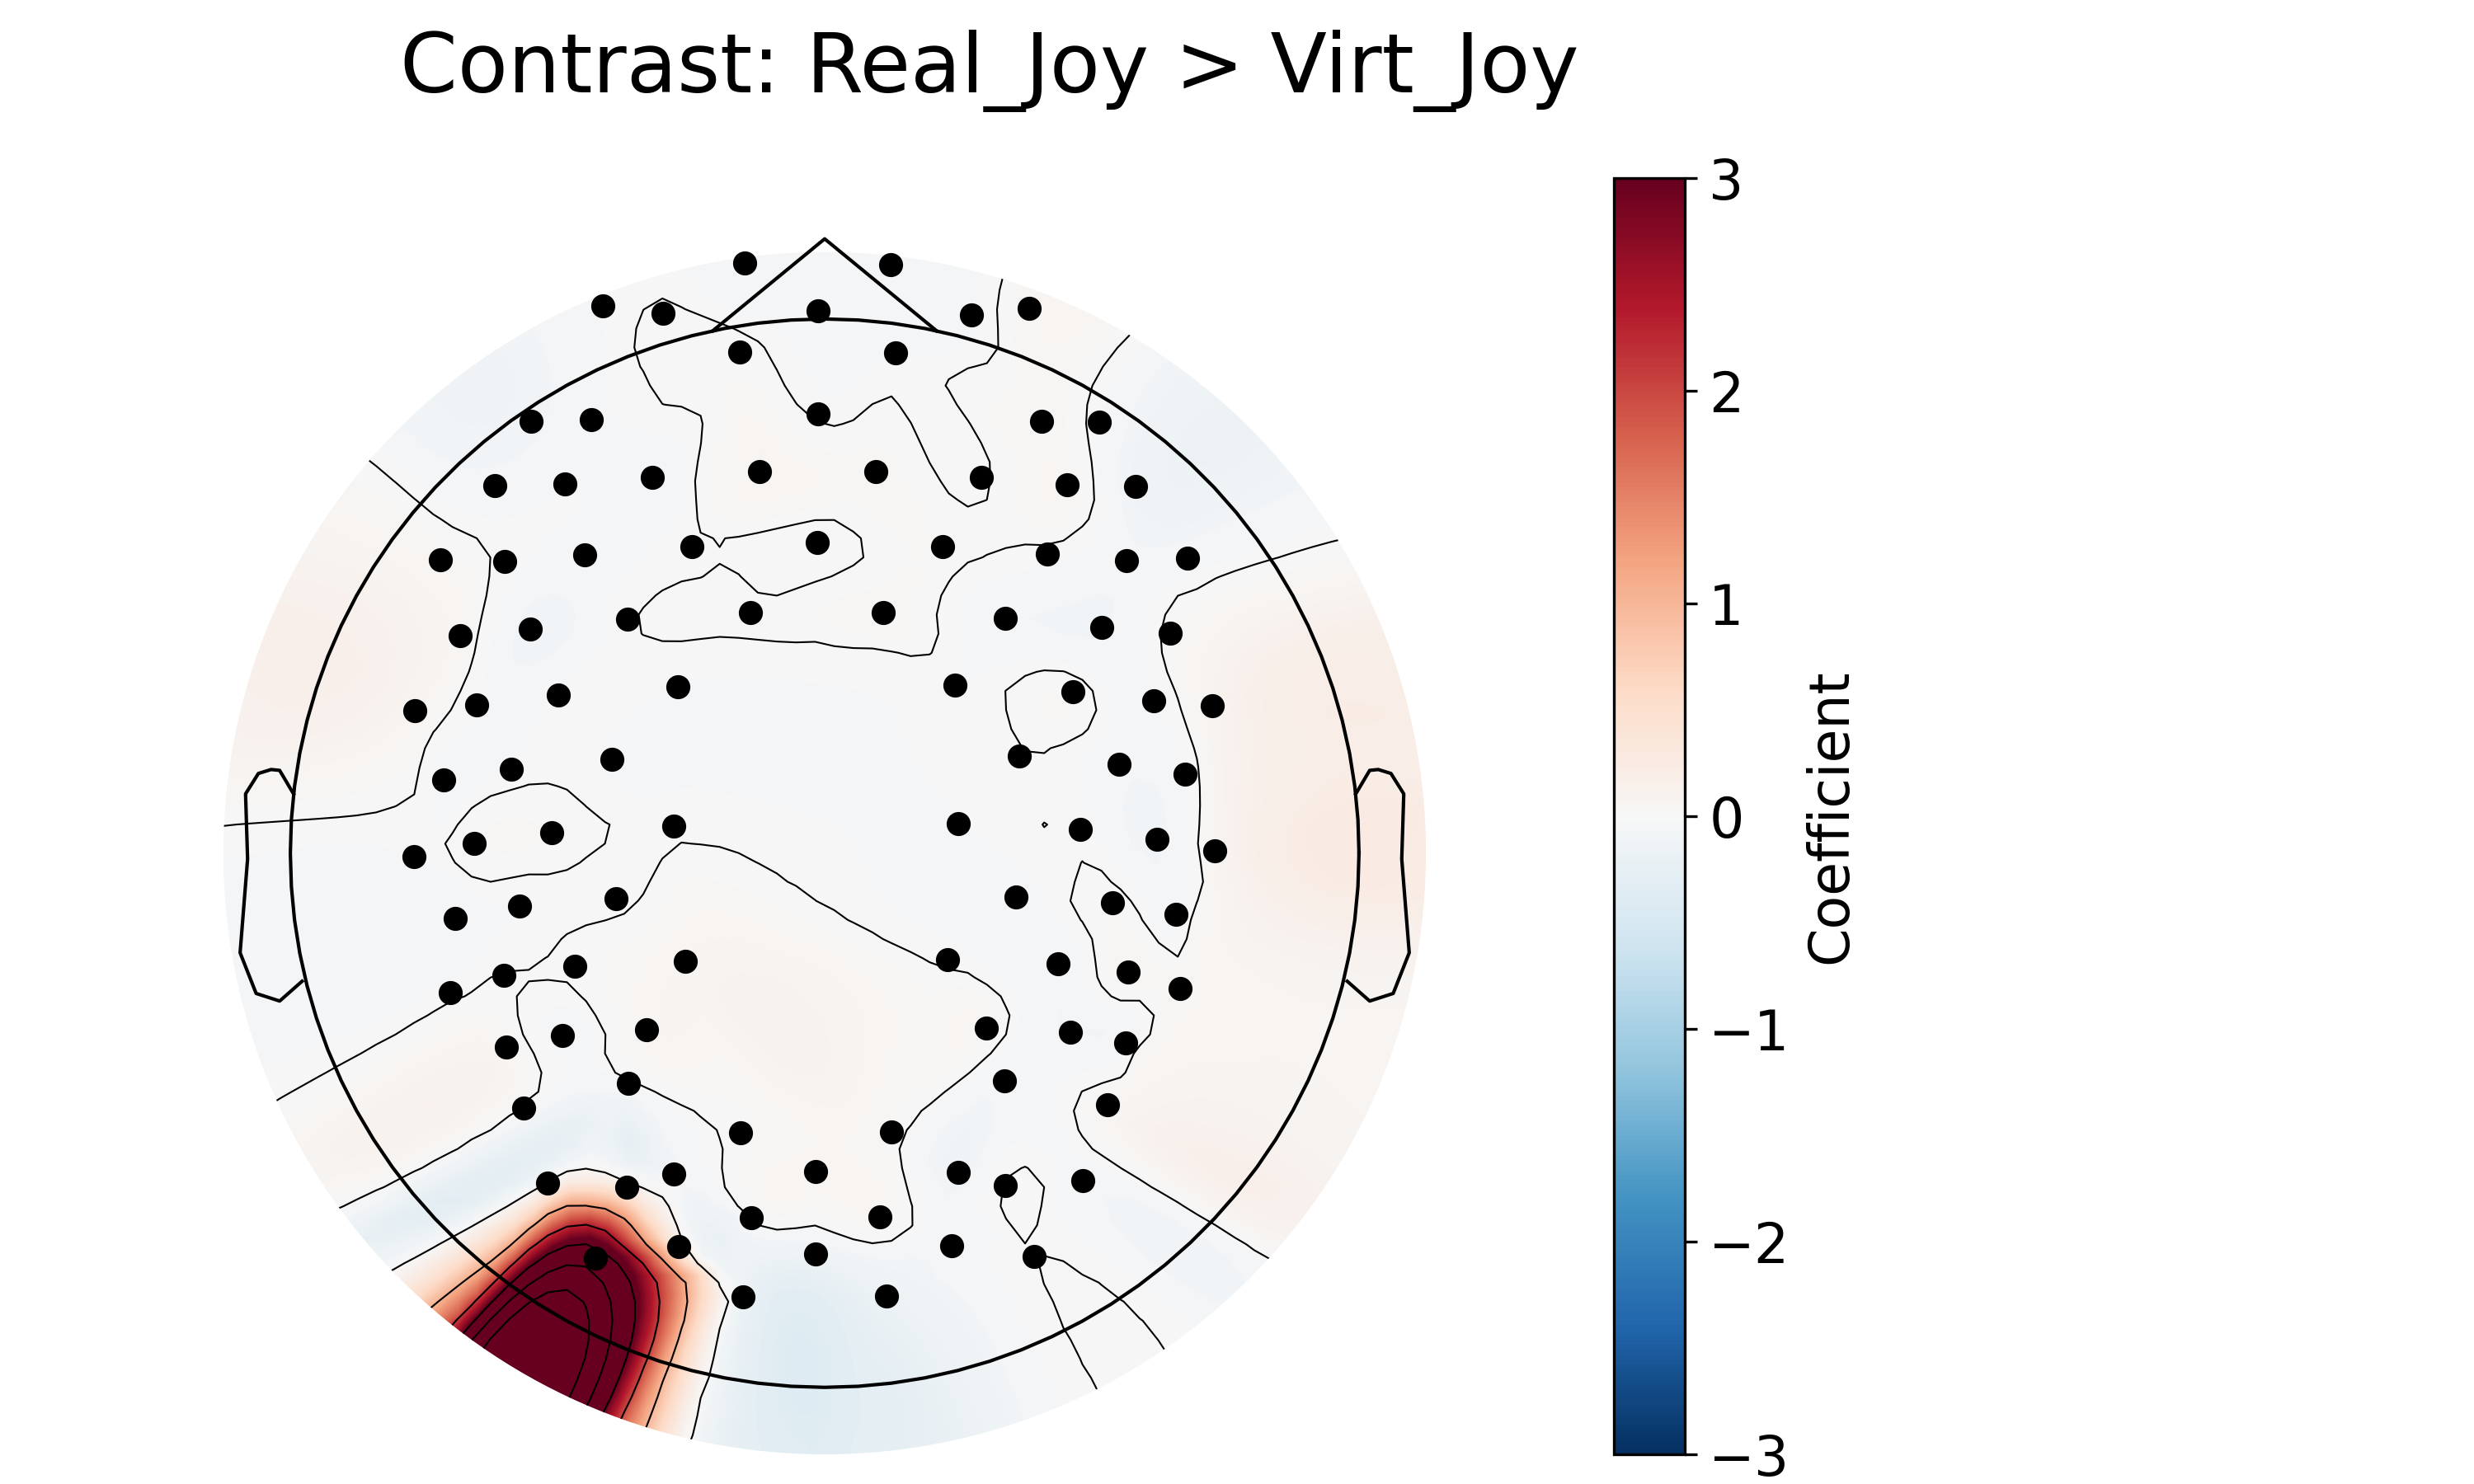
\includegraphics[width=0.45\textwidth]{C:/Users/super/OneDrive - Ontario Tech University/fNIRS_Emotions/plots/glm/contrasts/differences/Contrast_Real_Joy-Virt_Joy.png}
  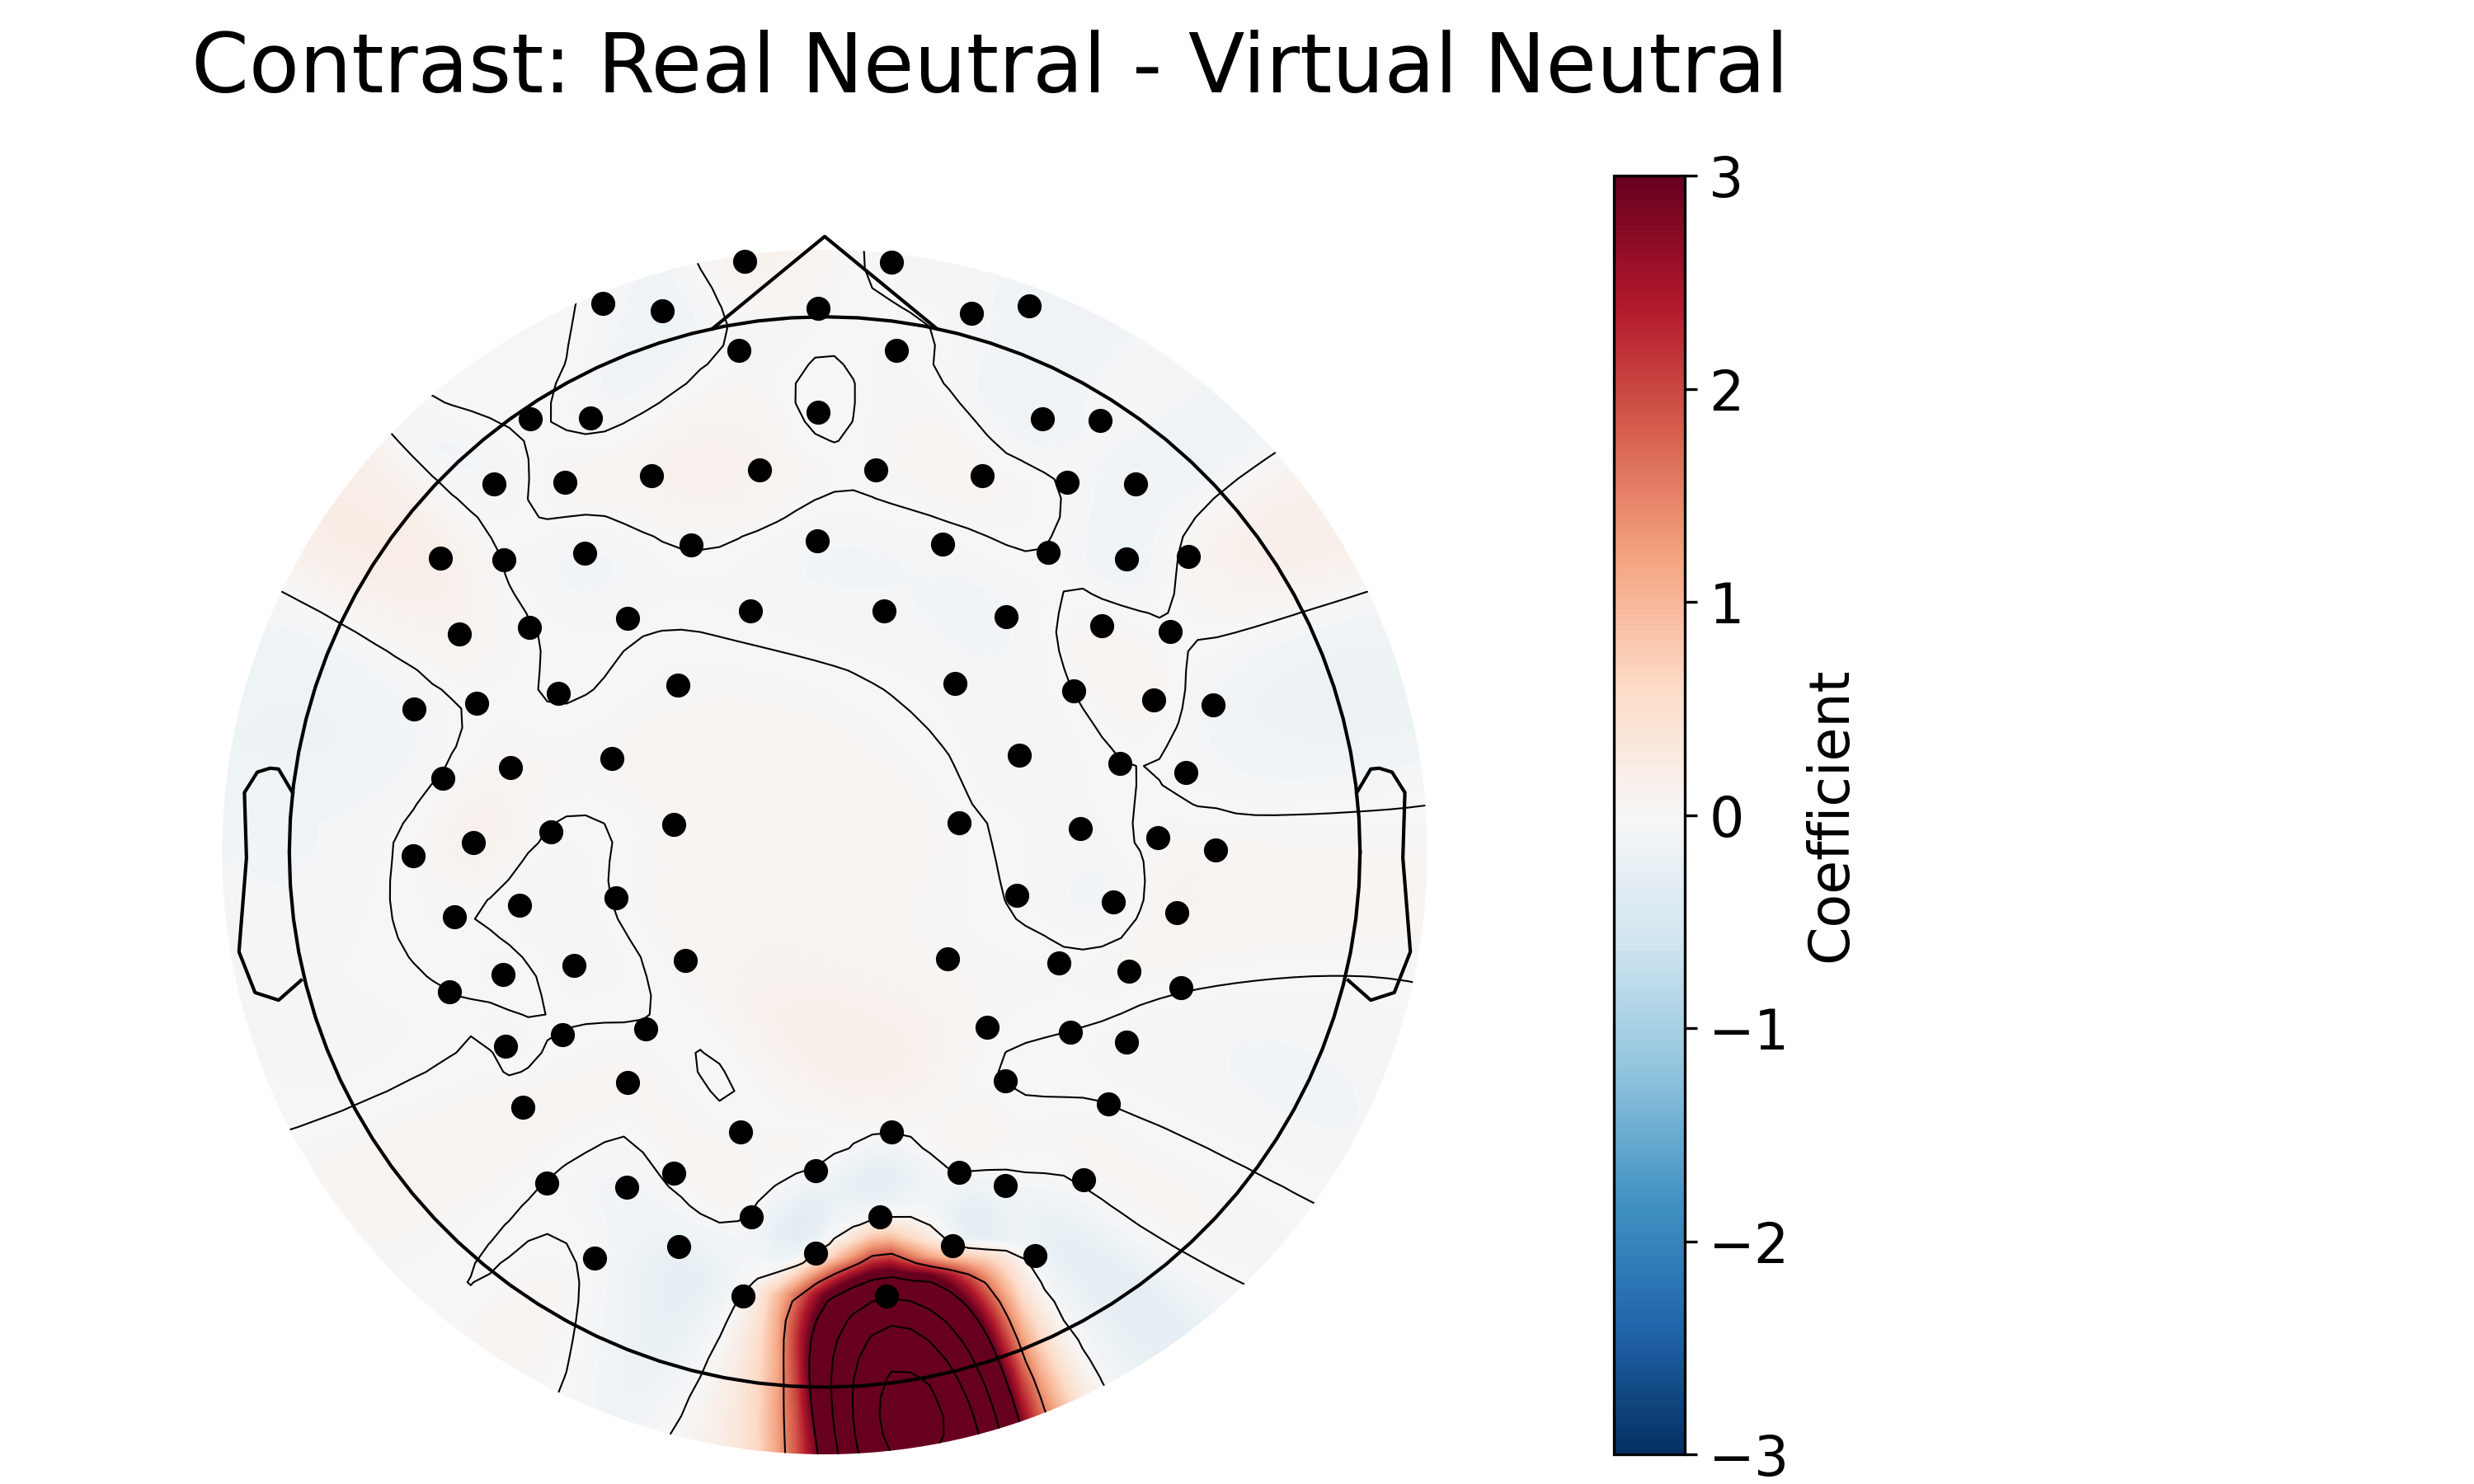
\includegraphics[width=0.45\textwidth]{C:/Users/super/OneDrive - Ontario Tech University/fNIRS_Emotions/plots/glm/contrasts/differences/Contrast_Real_Neutral-Virt_Neutral.png}
  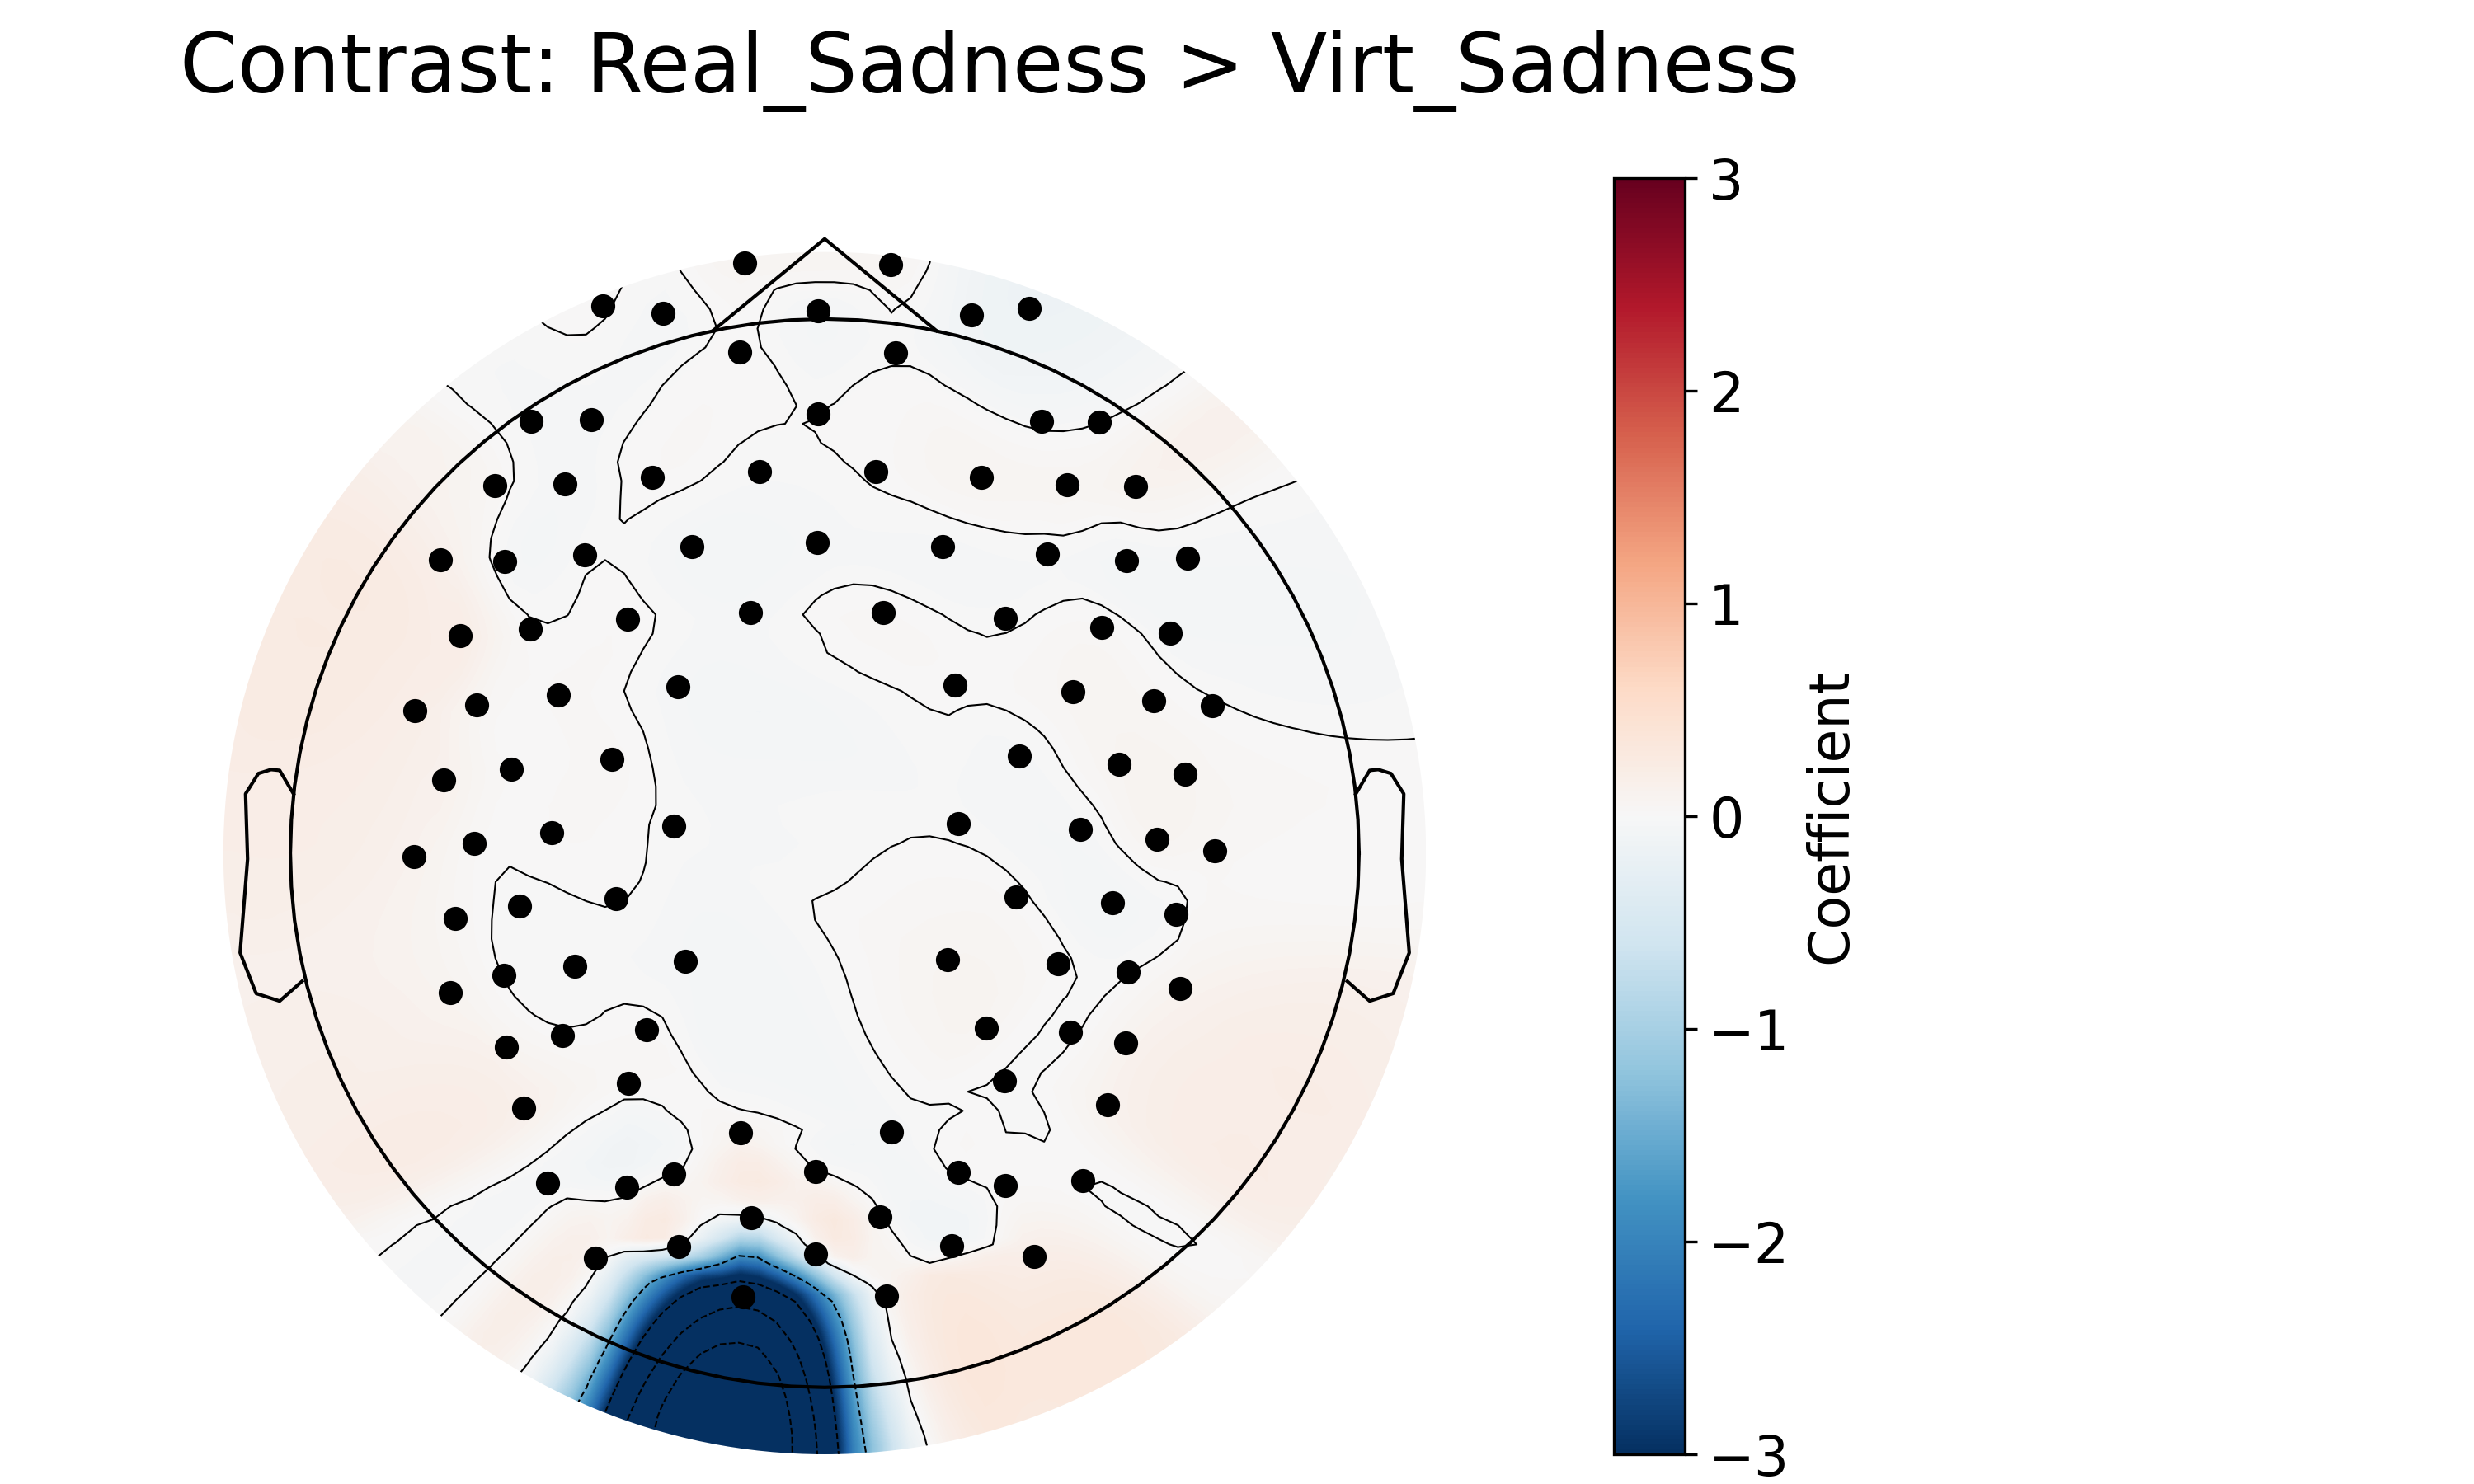
\includegraphics[width=0.45\textwidth]{C:/Users/super/OneDrive - Ontario Tech University/fNIRS_Emotions/plots/glm/contrasts/differences/Contrast_Real_Sadness-Virt_Sadness.png}
  \caption[GLM: Face Type \texorpdfstring{$\times$}{x} Emotion Contrasts]{GLM results for the contrast between real and virtual conditions within each emotion.
  Same concept as explained in figure \ref{fig:glm_real_vs_virtual}. }
  \label{fig:glm_real_vs_virtual_emotion_analysis}
\end{figure}

The interaction of face type with emotion (Real $>$ Virt within each emotion as shown in \ref{fig:glm_real_vs_virtual_emotion_analysis}) revealed significant differences in occipital regions exclusively.
In the case of disgust, real faces elicited greater activation in the right occipital region compared to virtual faces, while the left occipital region showed the opposite pattern.
For Joy and Neutral emotions, real faces also elicited greater activation in the occipital regions compared to virtual faces.
For Sadness, the left occipital region showed greater activation for virtual faces compared to real faces.
These findings suggest that the neural response to emotional expressions is modulated by the realism of the face stimuli. 

The full table of the GLM contrasts for all main effects and interactions can be found in Appendix \ref{tab:appendix_glm_results}.

\section{Functional Connectivity Results}
\subsection{Face Type Contrasts}
\begin{figure}[H]
  \centering
  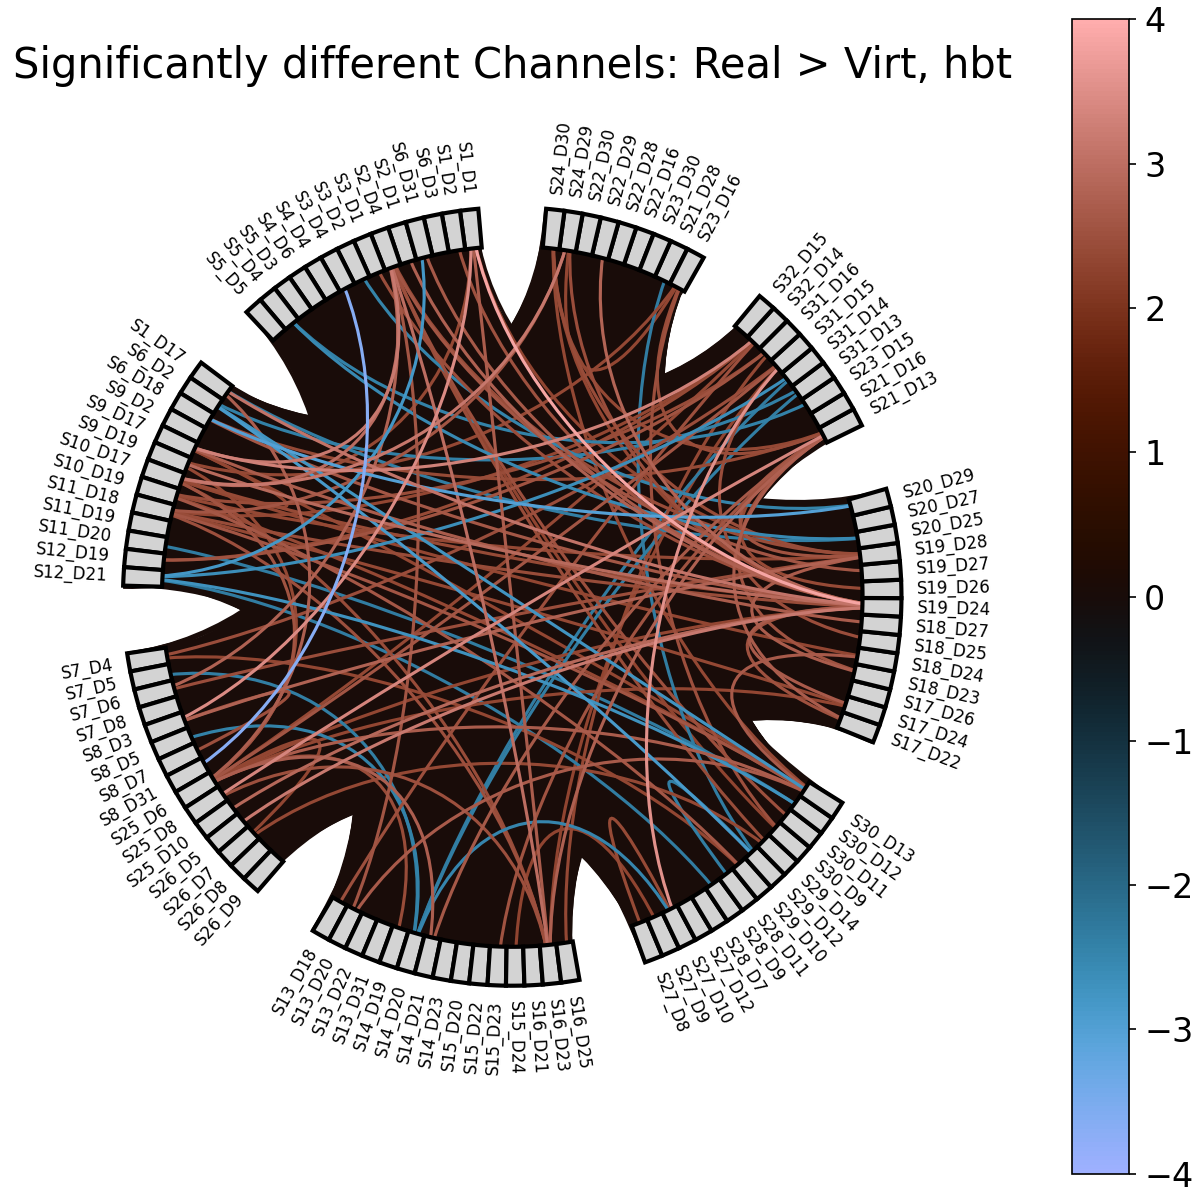
\includegraphics[width=0.85\textwidth]{C:/Users/super/OneDrive - Ontario Tech University/fNIRS_Emotions/plots/spectral_connectivity_time/chord_plots/group_level_t_tests_roi/face_type_Real_Virt.png}
  \caption[FC: Real vs. Virtual]{Functional connectivity results for the contrast between real and virtual conditions.
  Red signifies that condition 1 (real faces) has higher connectivity between those two ROI's than condition 2 (virtual faces), while blue signifies that condition 2 (virtual faces) has higher connectivity than condition 1 (real faces).
  The color bar on the right shows the $t$-statistic of the contrast, which indicates the strength of the difference in connectivity between the two conditions.
  The Mean $t$-value across ROI's is the average of the $t$-values for all significant channel pairs across all ROI's, and generally indicates whether the connectivity is higher or lower in one condition compared to the other.
  If this value is positive, it indicates that the connectivity is higher in condition 1 (real faces) than condition 2 (virtual faces), and vice versa.}
  \label{fig:fc_real_vs_virtual}
\end{figure}

The main effect of real versus virtual faces (as shown in \ref{fig:fc_real_vs_virtual}) for functional connectivity revealed significant differences in connectivity between real and virtual faces across ROI's.
Most ROI's showed higher connectivity for real faces compared to virtual faces, with a few exceptions, i.e. the left occipital/parietal ROI, which showed higher connectivity for virtual faces compared to real faces.
A mean $t$-value of 1.55 indicates that the connectivity is generally higher for real faces compared to virtual faces across all ROI's. 

\subsection{Emotion Contrasts}
\begin{figure}[H]
  \centering
  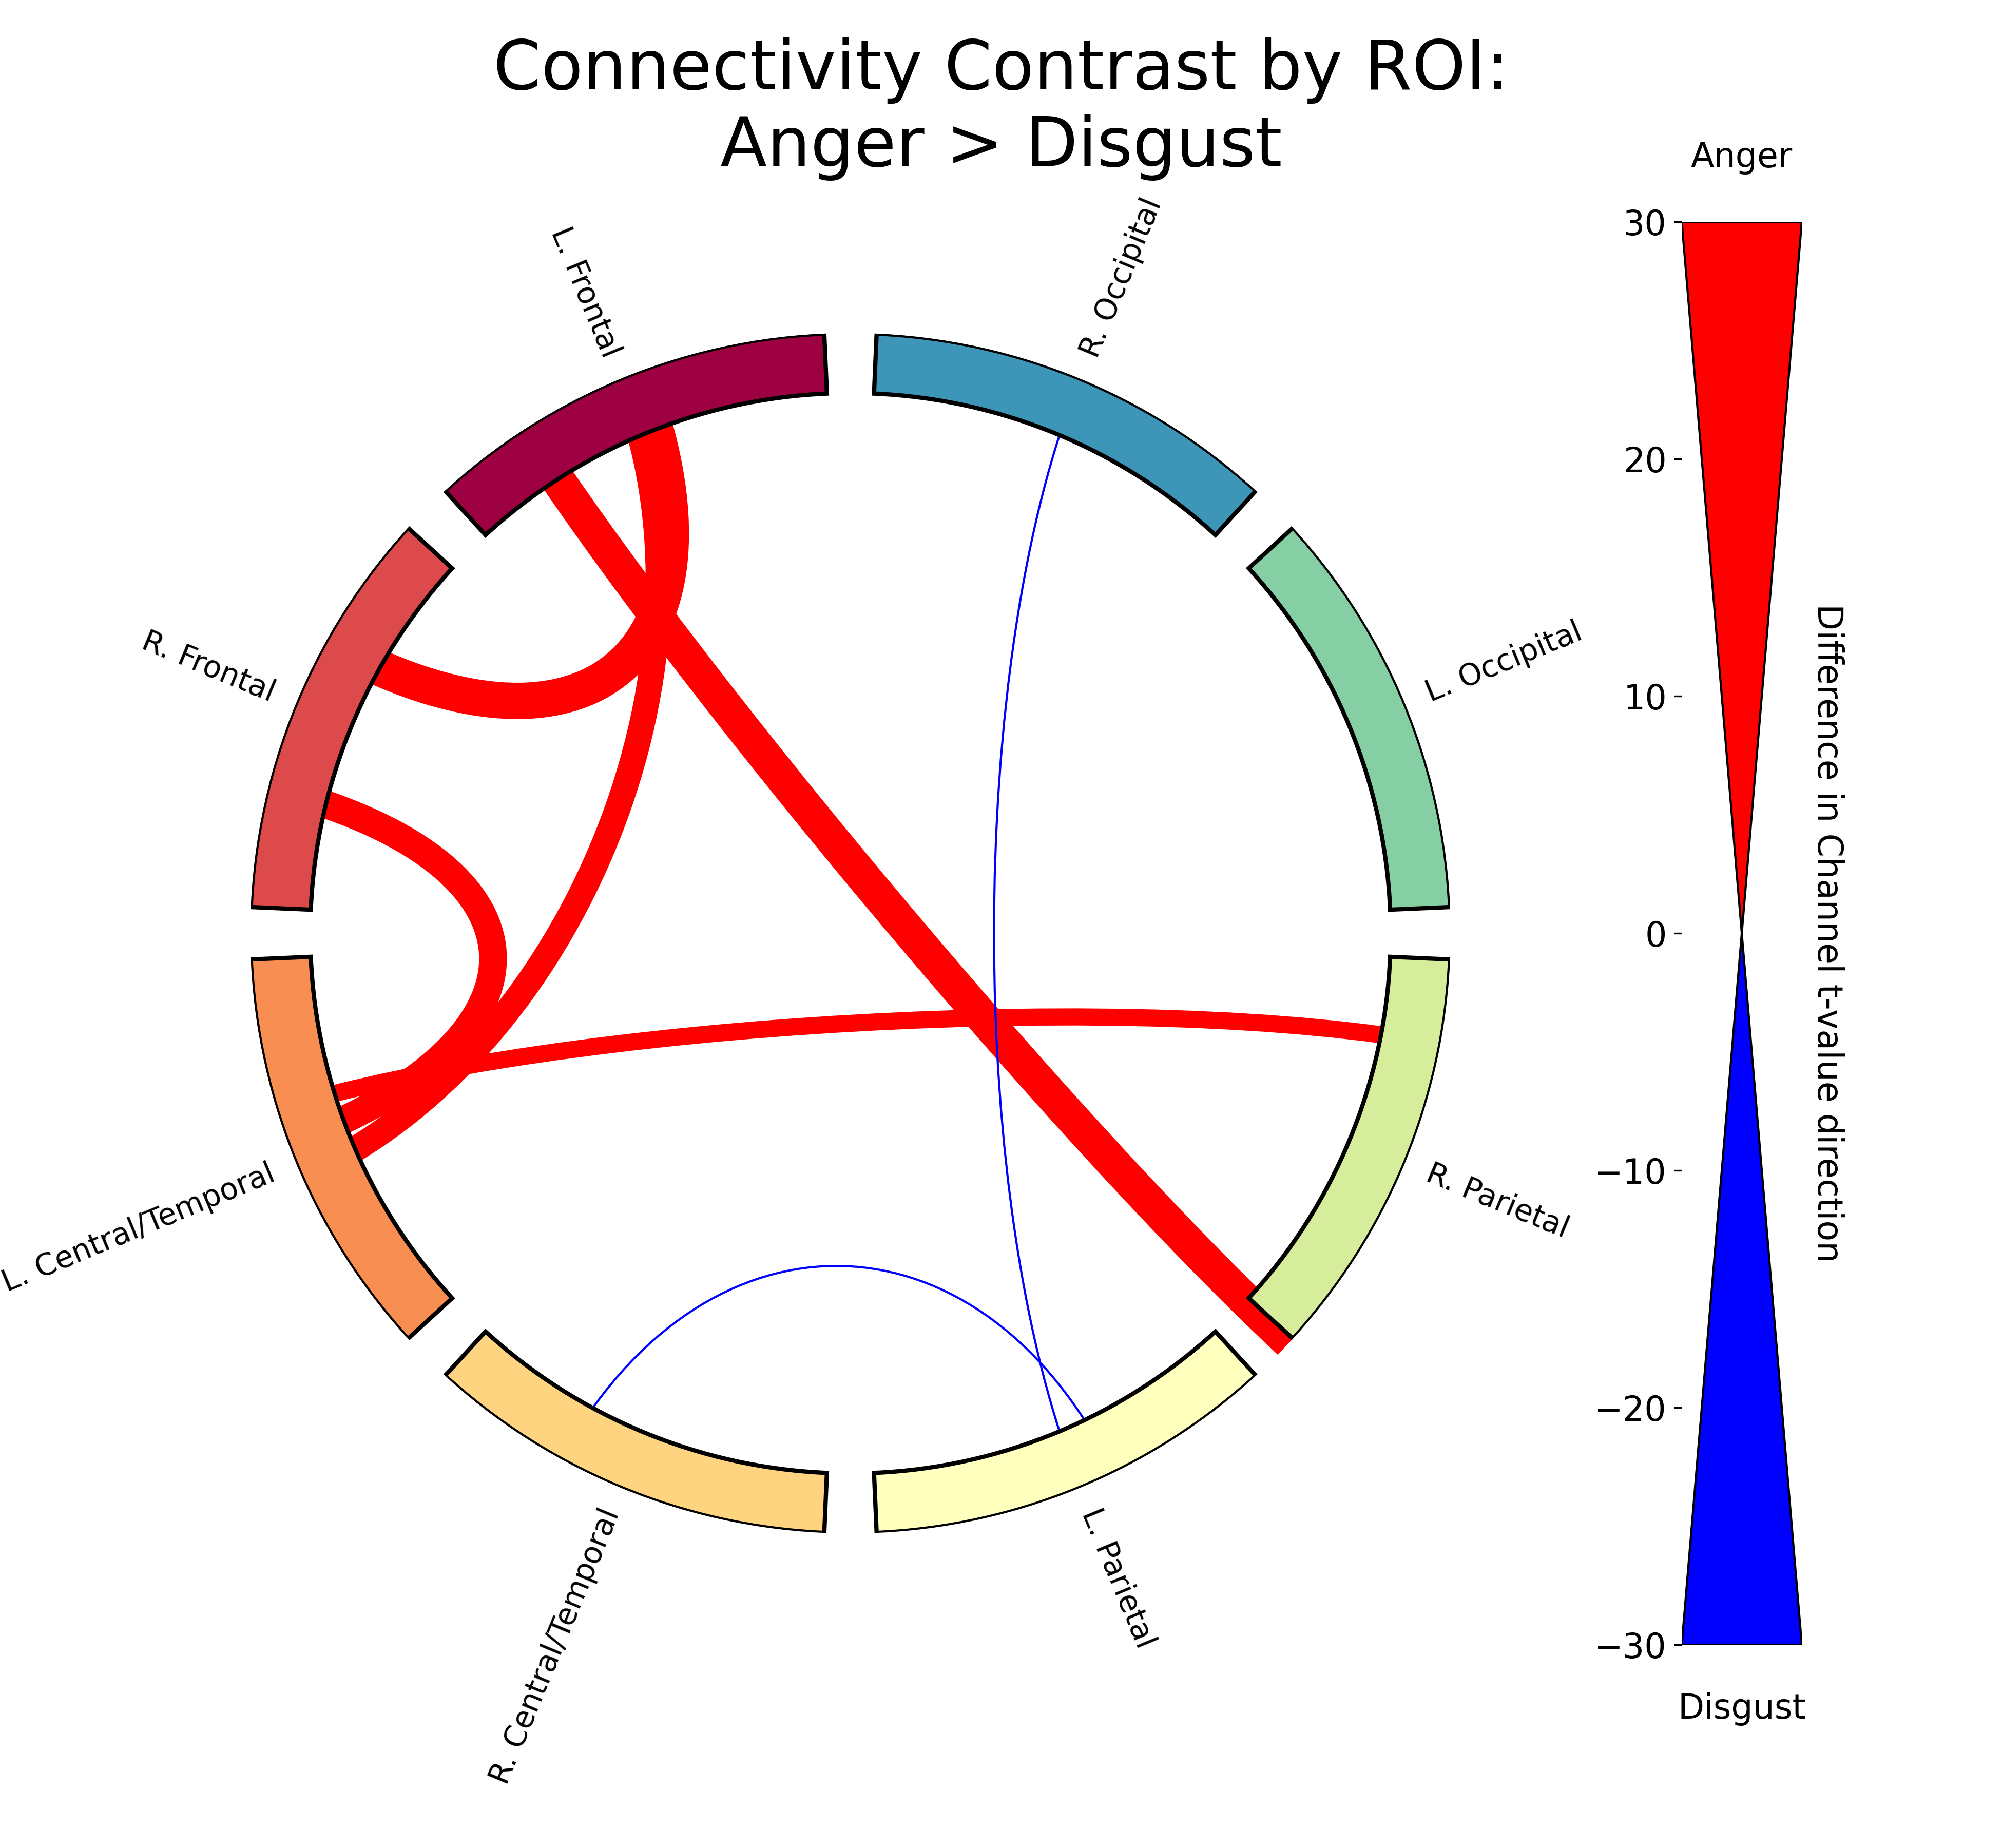
\includegraphics[width=0.24\textwidth]{C:/Users/super/OneDrive - Ontario Tech University/fNIRS_Emotions/plots/spectral_connectivity_time/chord_plots/group_level_t_tests_roi/emotion_Anger_Disgust.png}
  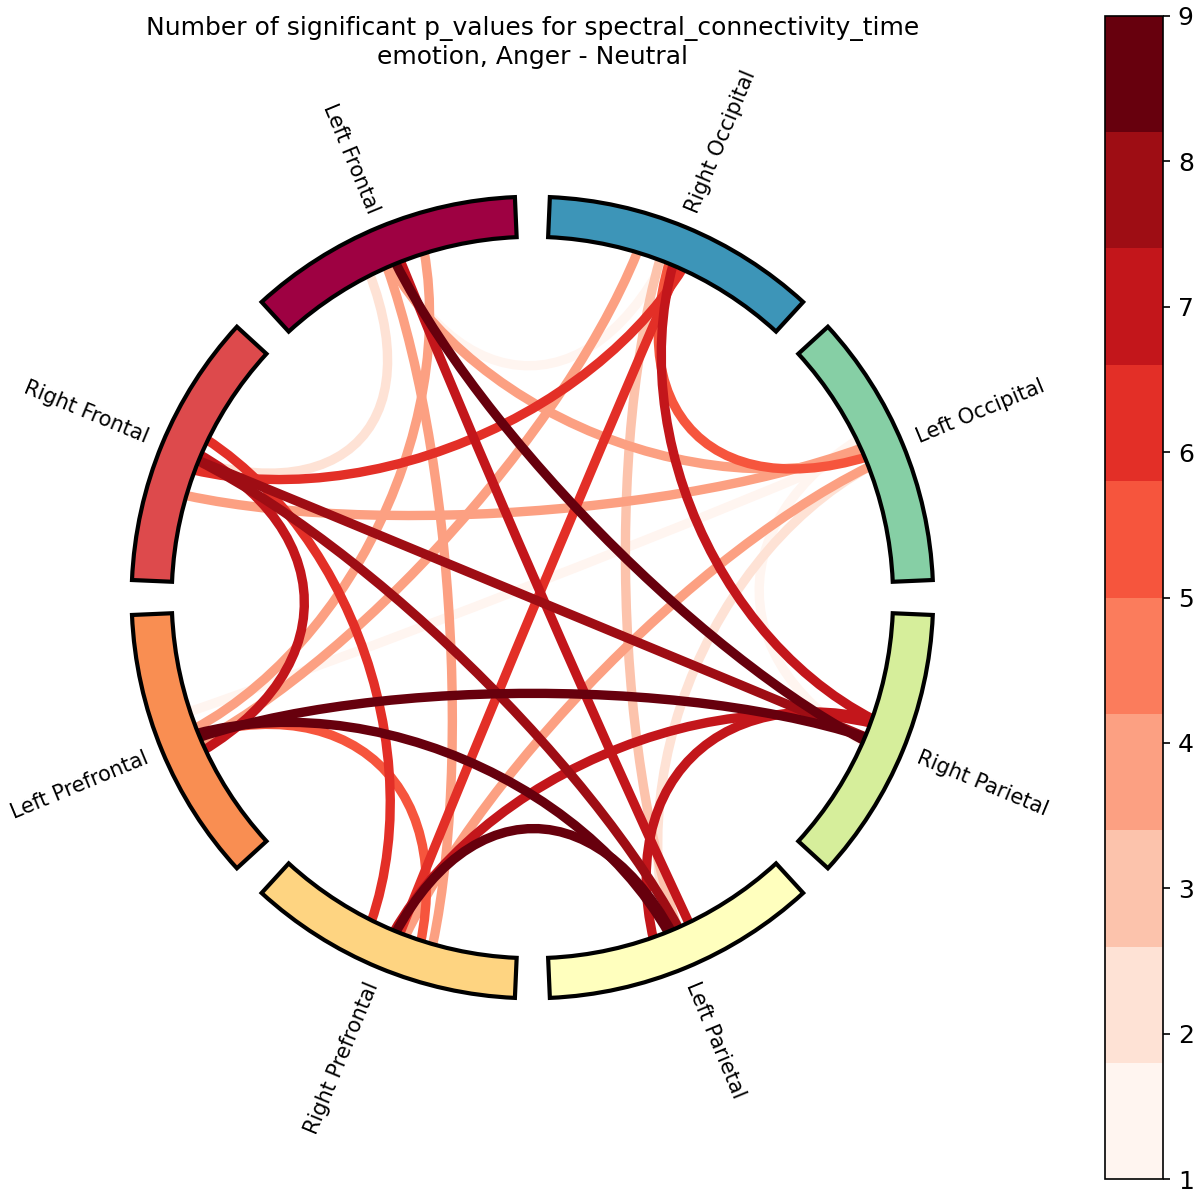
\includegraphics[width=0.24\textwidth]{C:/Users/super/OneDrive - Ontario Tech University/fNIRS_Emotions/plots/spectral_connectivity_time/chord_plots/group_level_t_tests_roi/emotion_Anger_Neutral.png}
  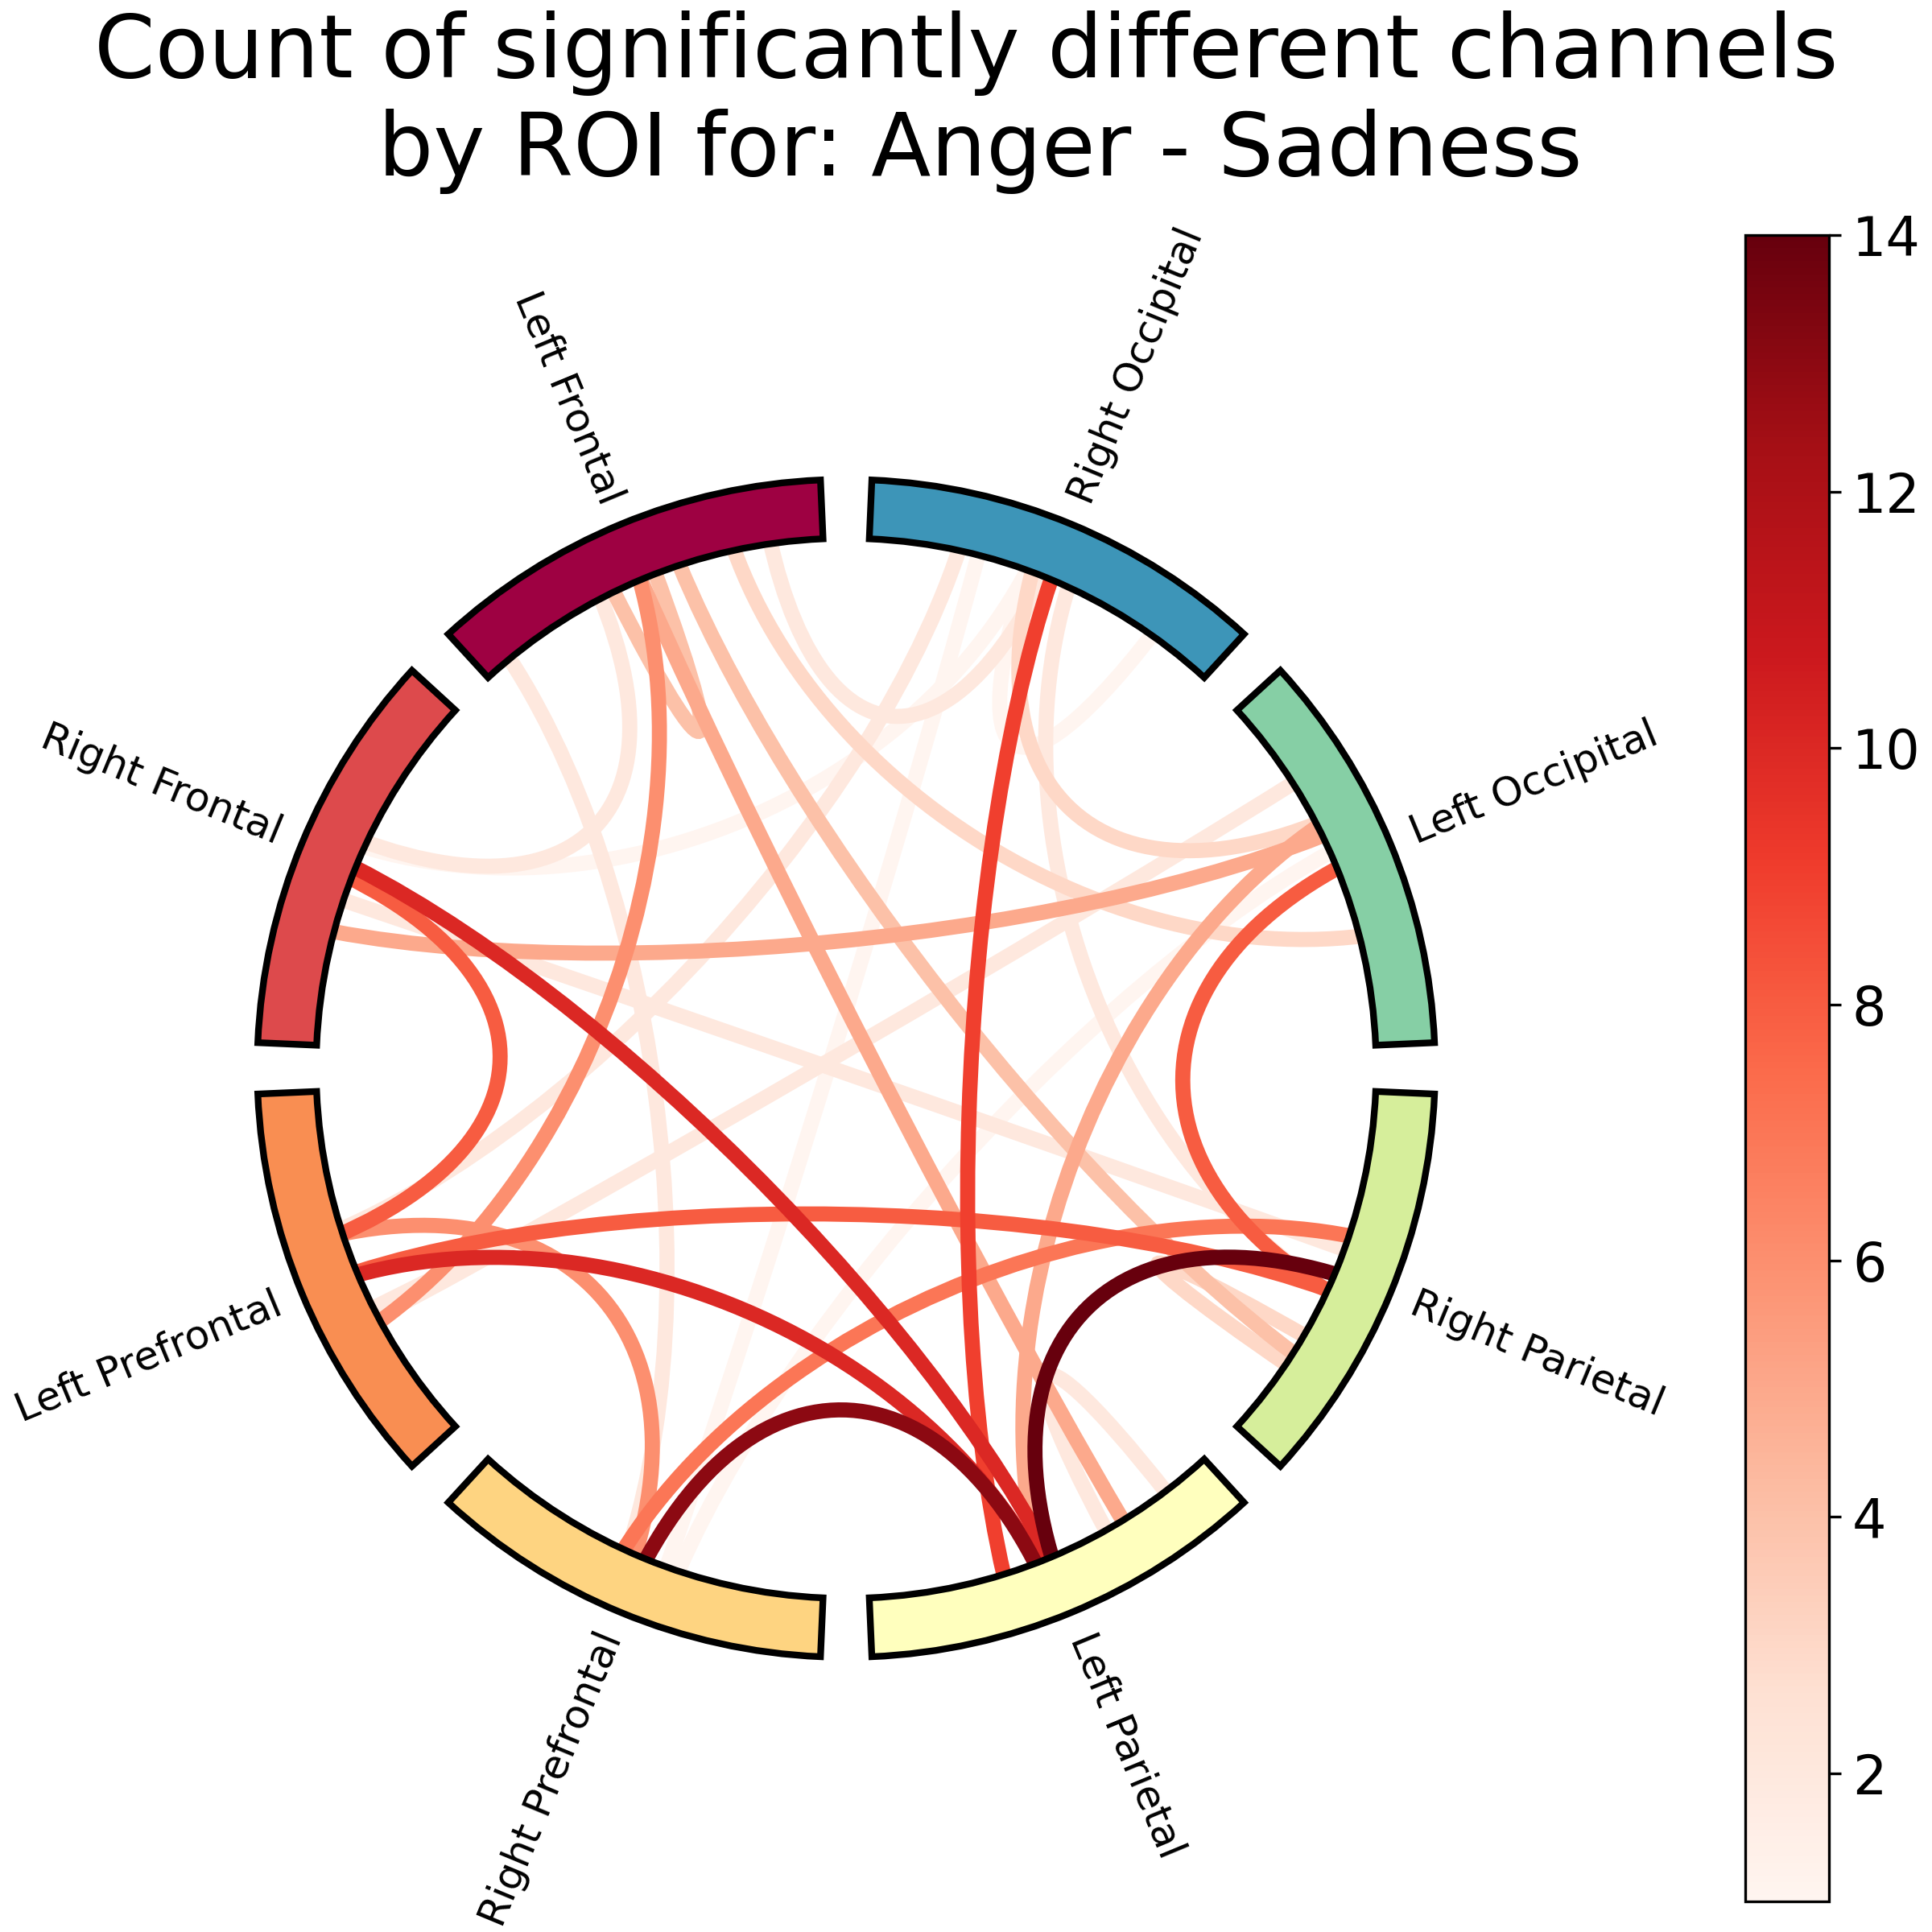
\includegraphics[width=0.24\textwidth]{C:/Users/super/OneDrive - Ontario Tech University/fNIRS_Emotions/plots/spectral_connectivity_time/chord_plots/group_level_t_tests_roi/emotion_Anger_Sadness.png}
  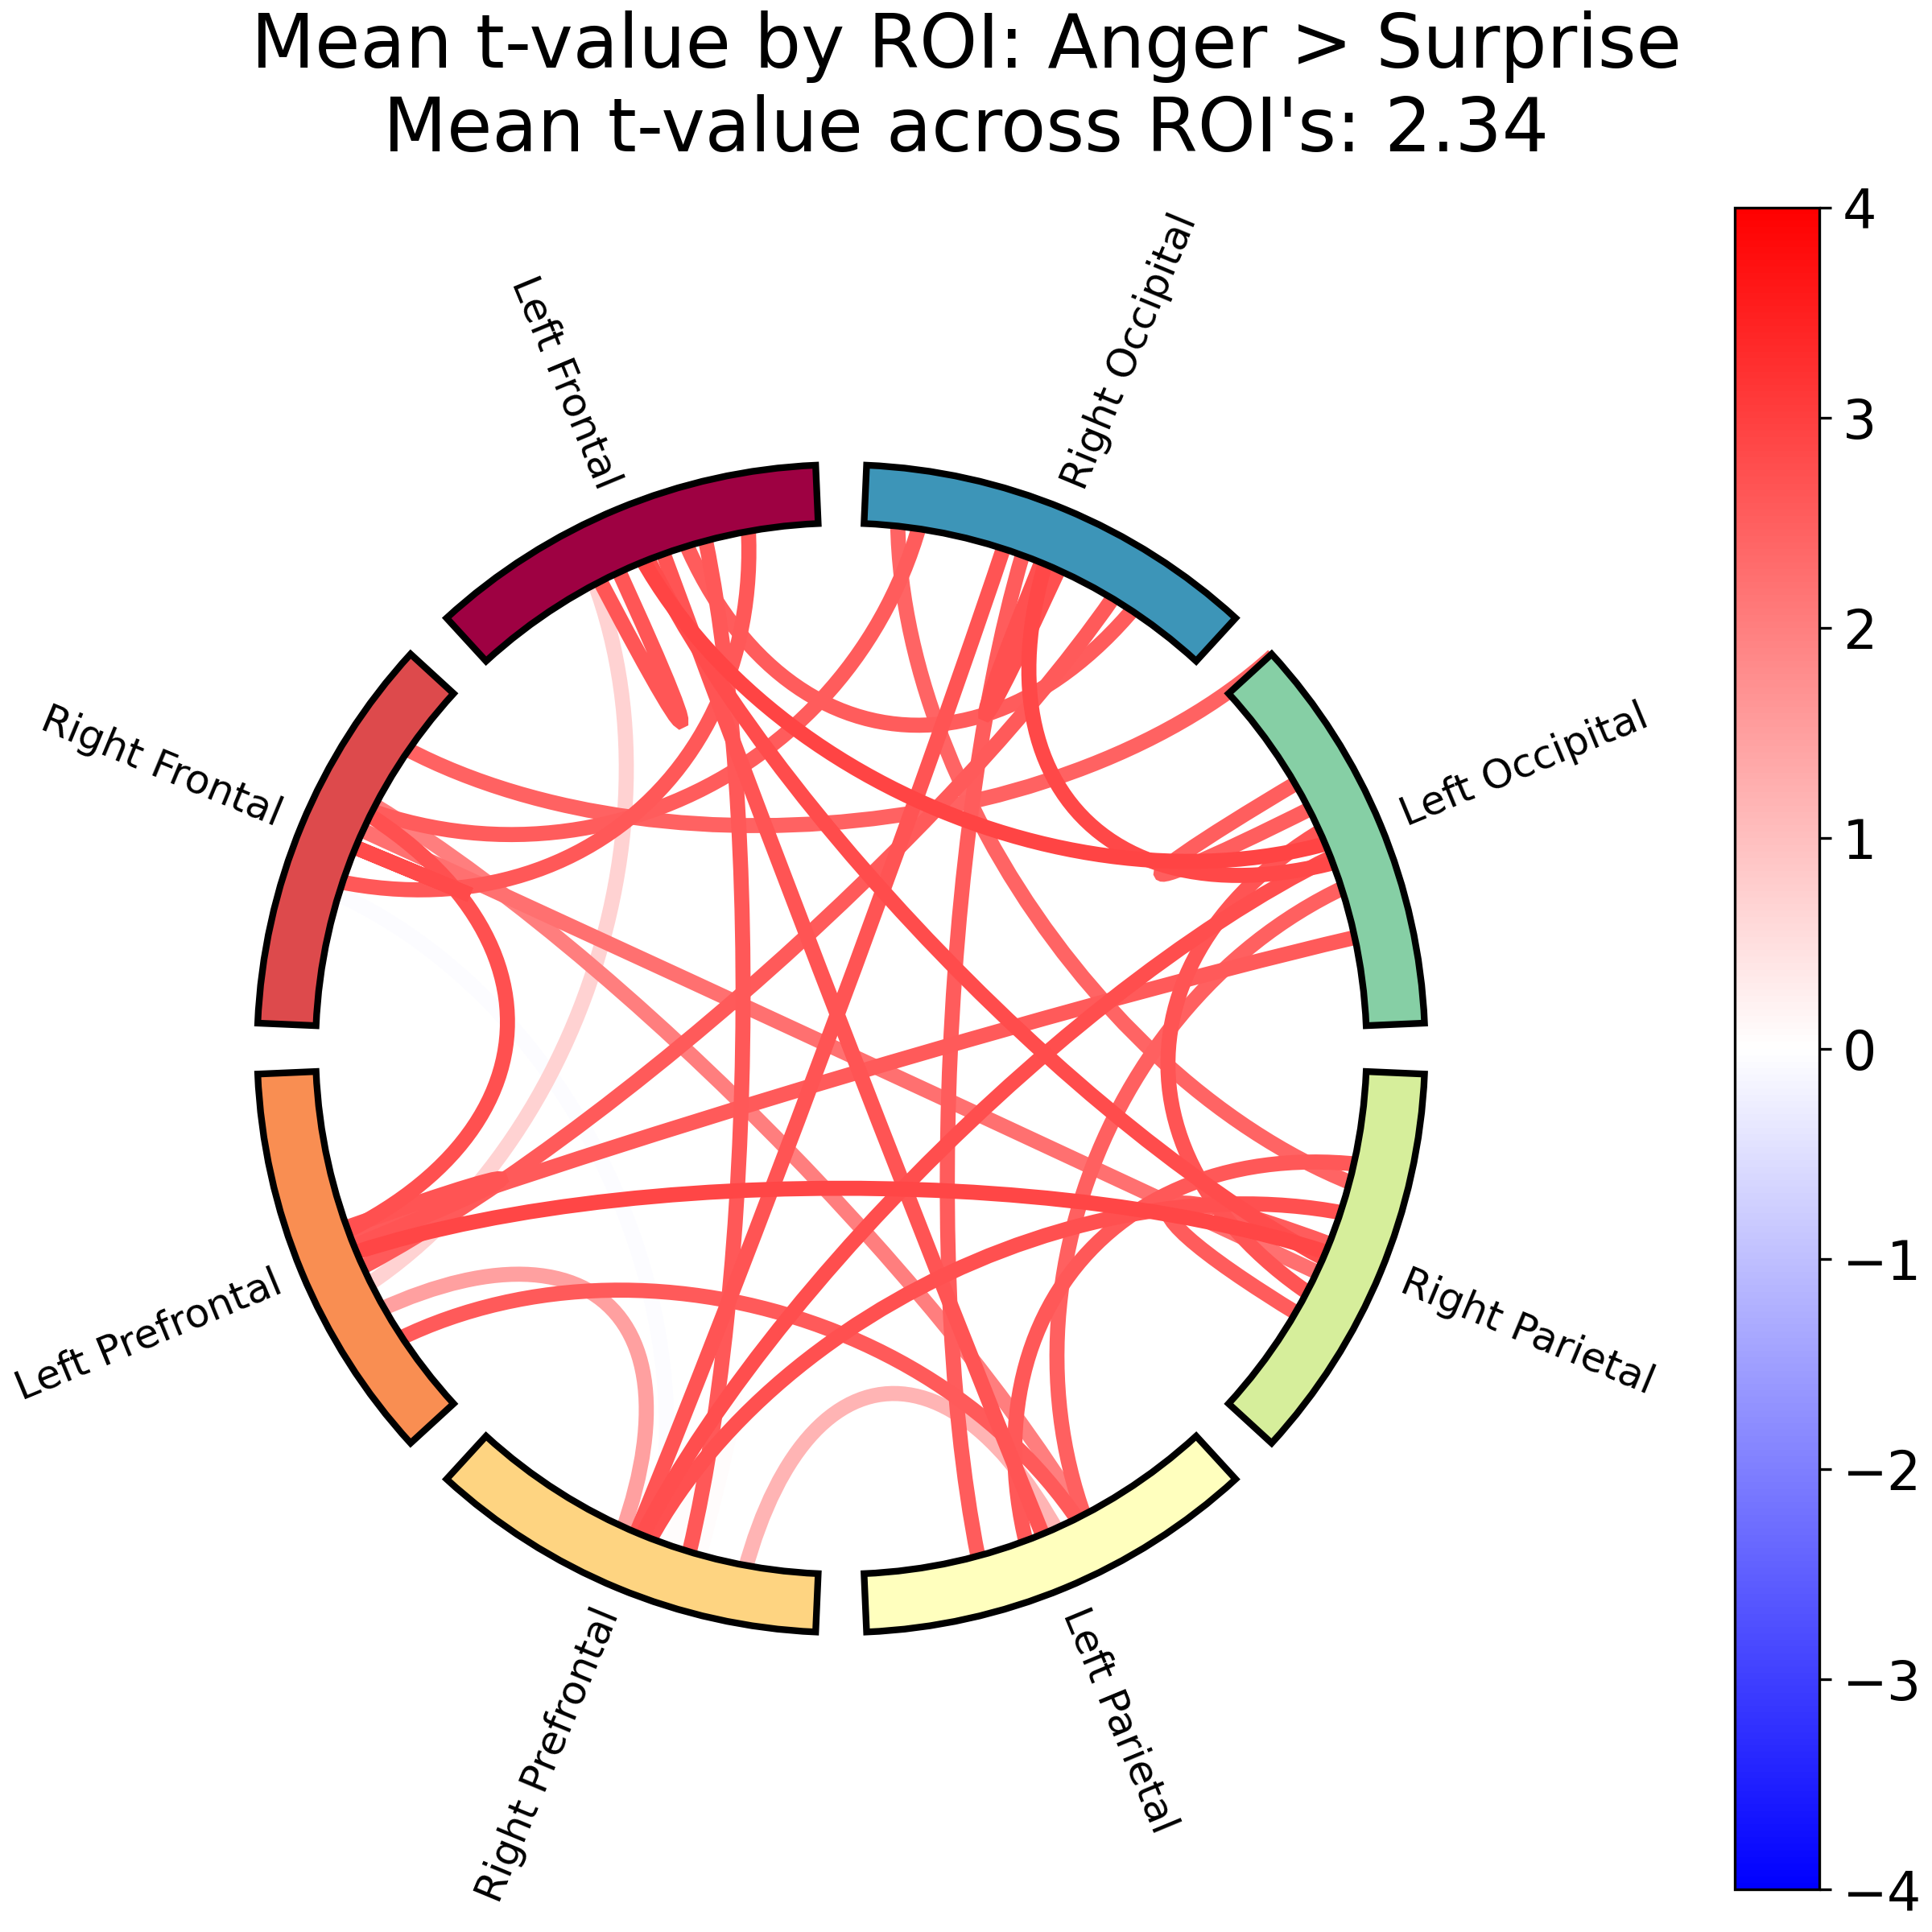
\includegraphics[width=0.24\textwidth]{C:/Users/super/OneDrive - Ontario Tech University/fNIRS_Emotions/plots/spectral_connectivity_time/chord_plots/group_level_t_tests_roi/emotion_Anger_Surprise.png}
  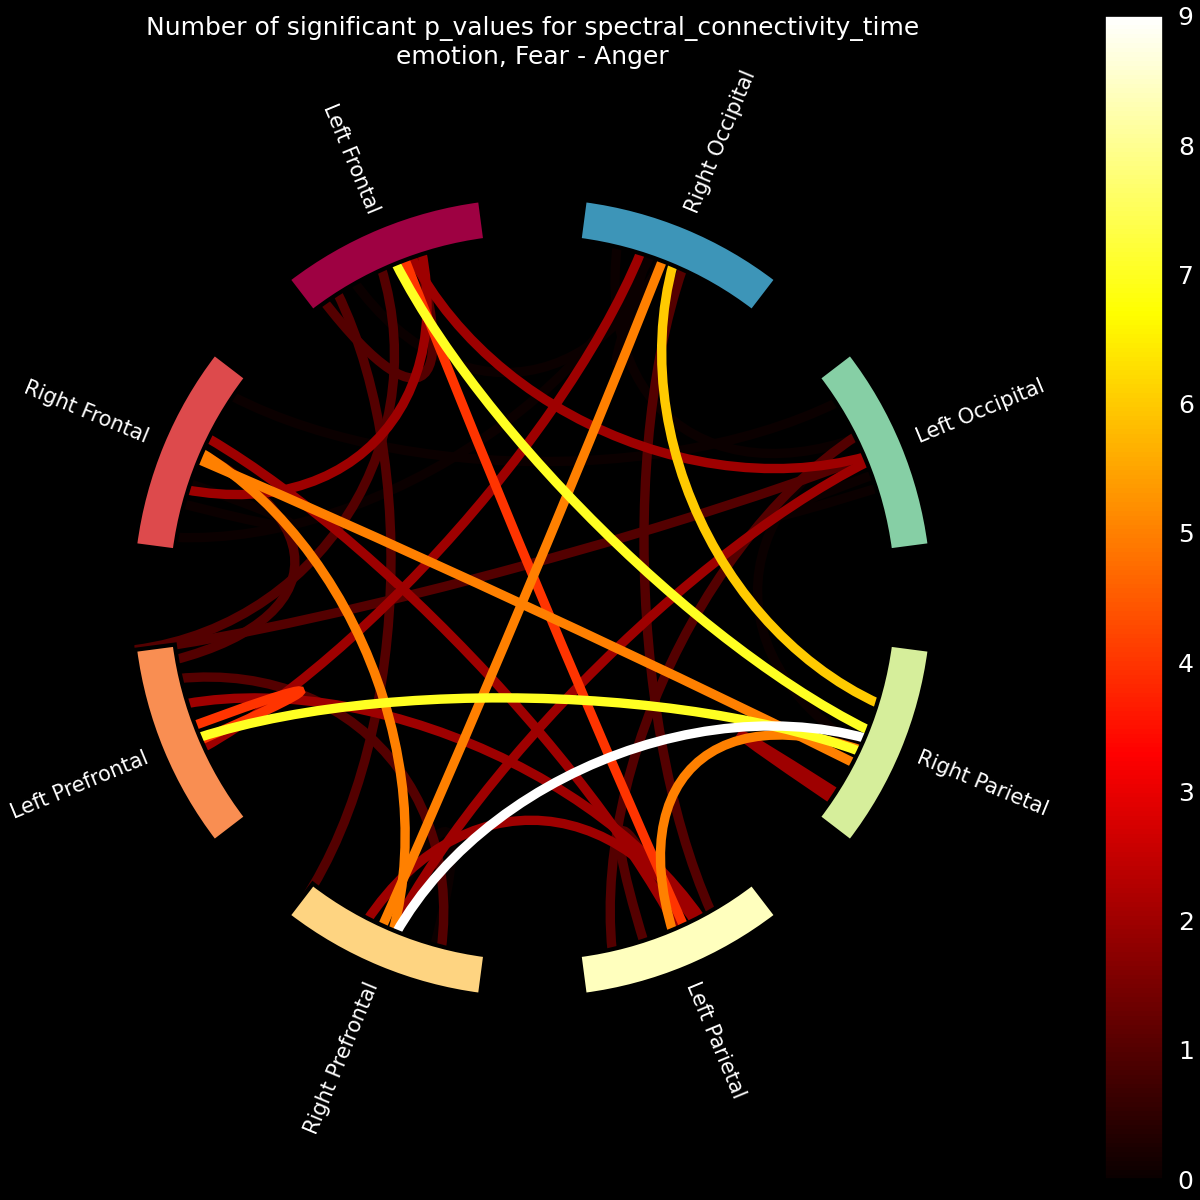
\includegraphics[width=0.24\textwidth]{C:/Users/super/OneDrive - Ontario Tech University/fNIRS_Emotions/plots/spectral_connectivity_time/chord_plots/group_level_t_tests_roi/emotion_Fear_Anger.png}
  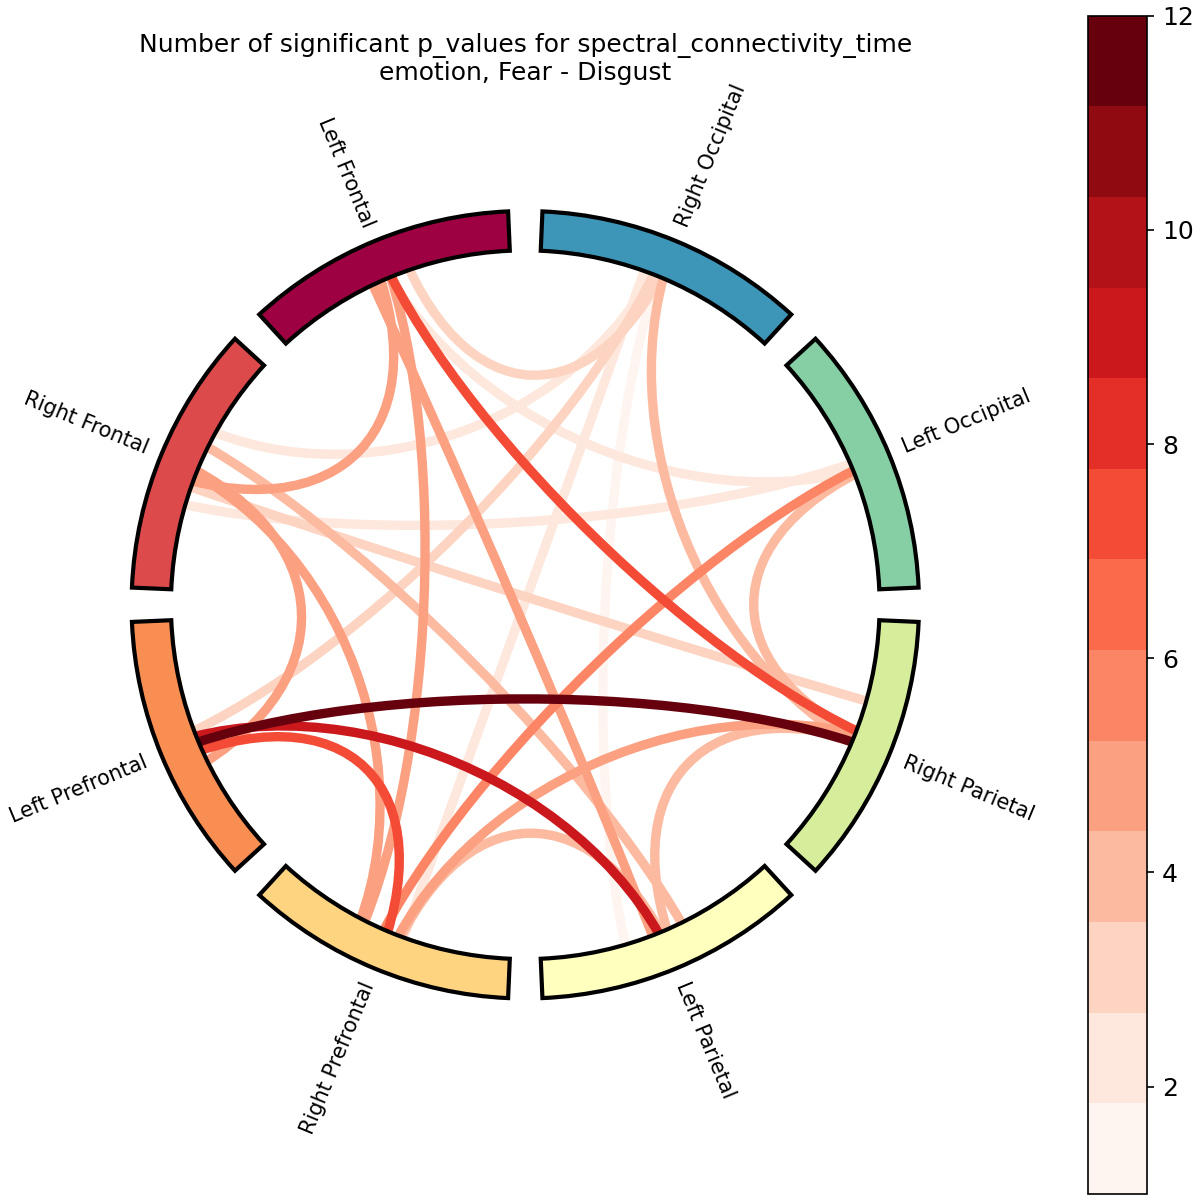
\includegraphics[width=0.24\textwidth]{C:/Users/super/OneDrive - Ontario Tech University/fNIRS_Emotions/plots/spectral_connectivity_time/chord_plots/group_level_t_tests_roi/emotion_Fear_Disgust.png}
  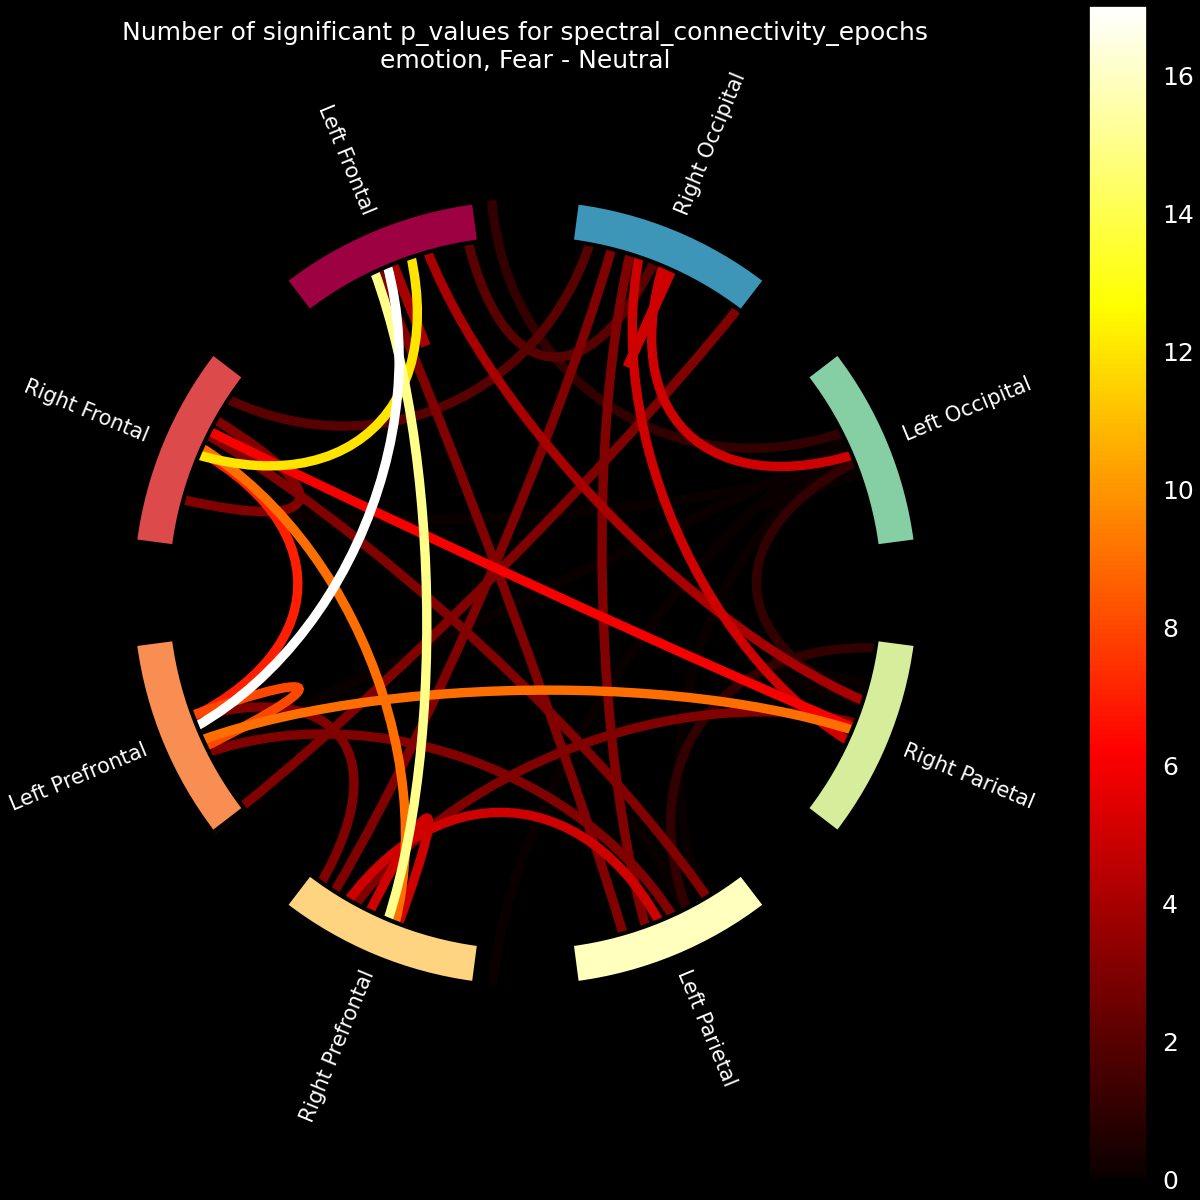
\includegraphics[width=0.24\textwidth]{C:/Users/super/OneDrive - Ontario Tech University/fNIRS_Emotions/plots/spectral_connectivity_time/chord_plots/group_level_t_tests_roi/emotion_Fear_Neutral.png}
  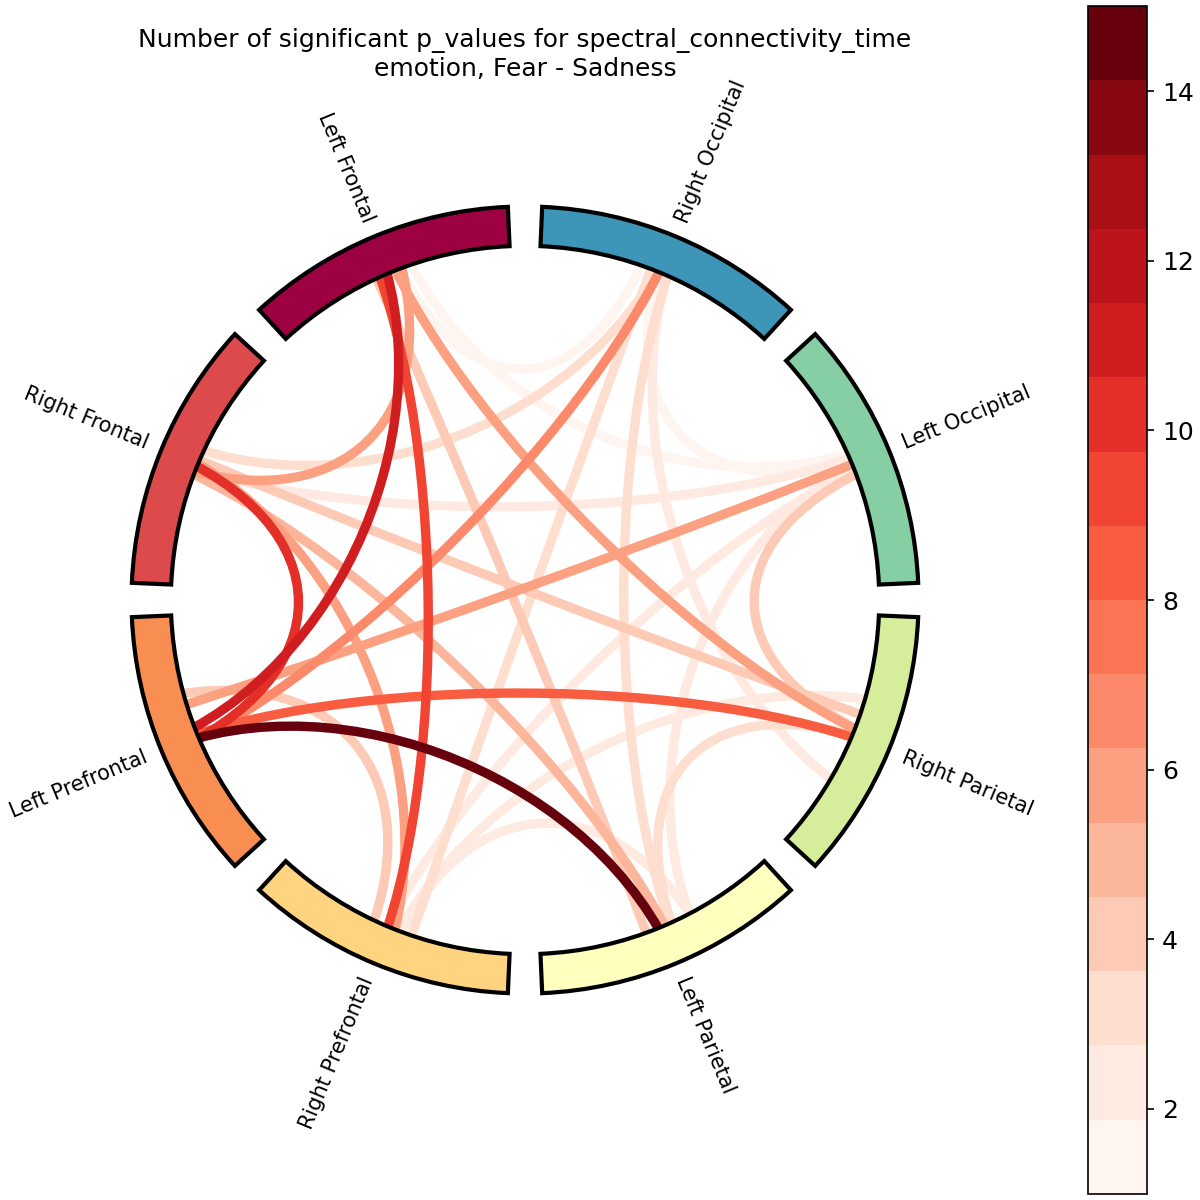
\includegraphics[width=0.24\textwidth]{C:/Users/super/OneDrive - Ontario Tech University/fNIRS_Emotions/plots/spectral_connectivity_time/chord_plots/group_level_t_tests_roi/emotion_Fear_Sadness.png}
  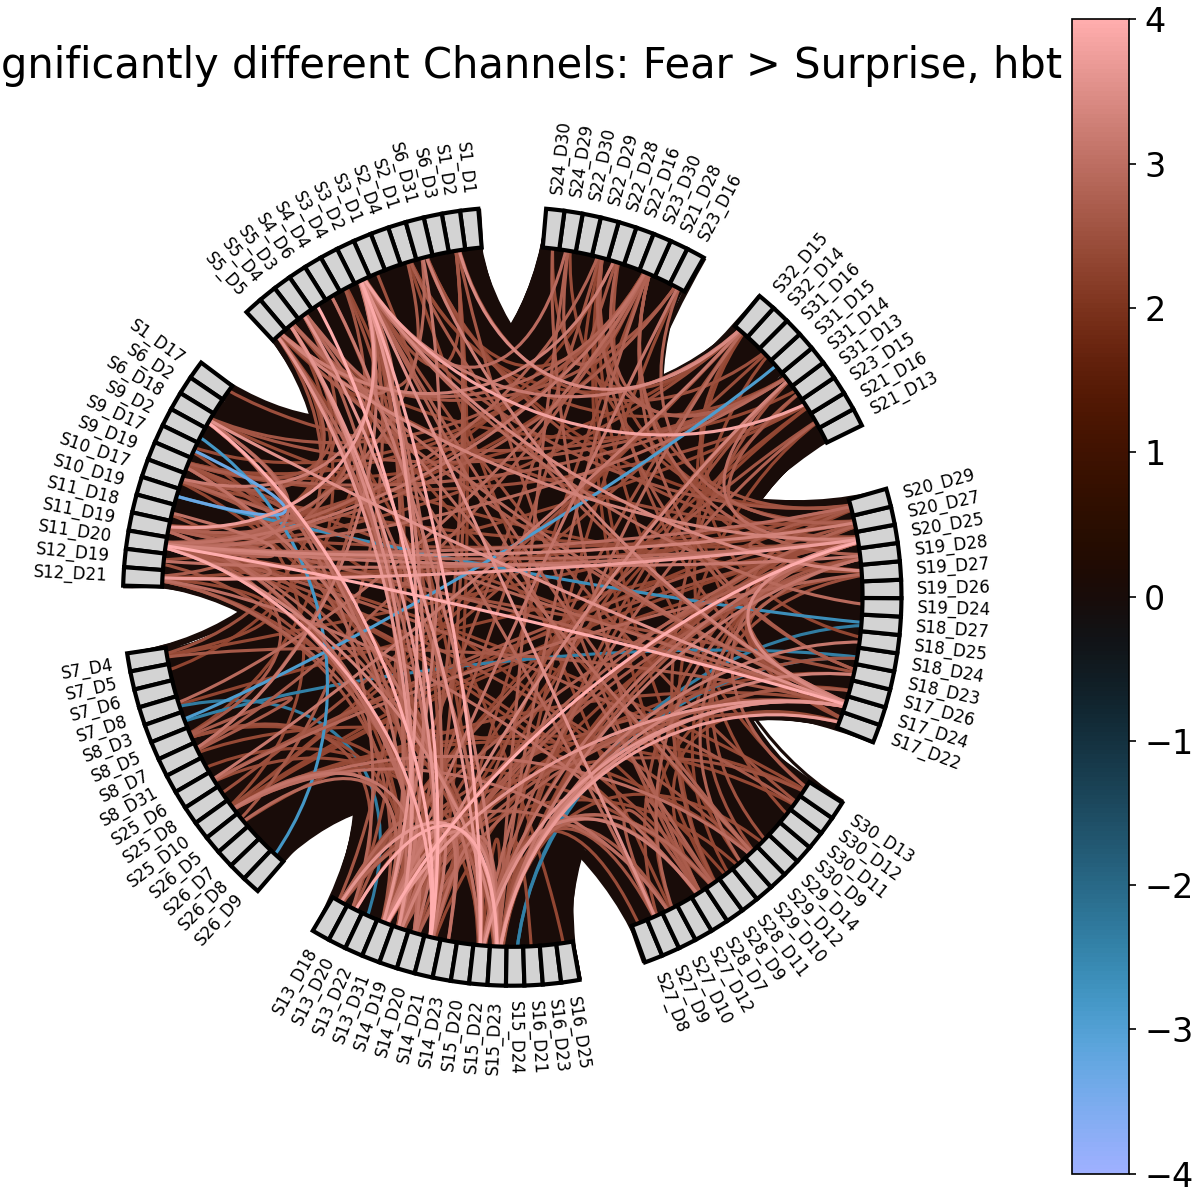
\includegraphics[width=0.24\textwidth]{C:/Users/super/OneDrive - Ontario Tech University/fNIRS_Emotions/plots/spectral_connectivity_time/chord_plots/group_level_t_tests_roi/emotion_Fear_Surprise.png}
  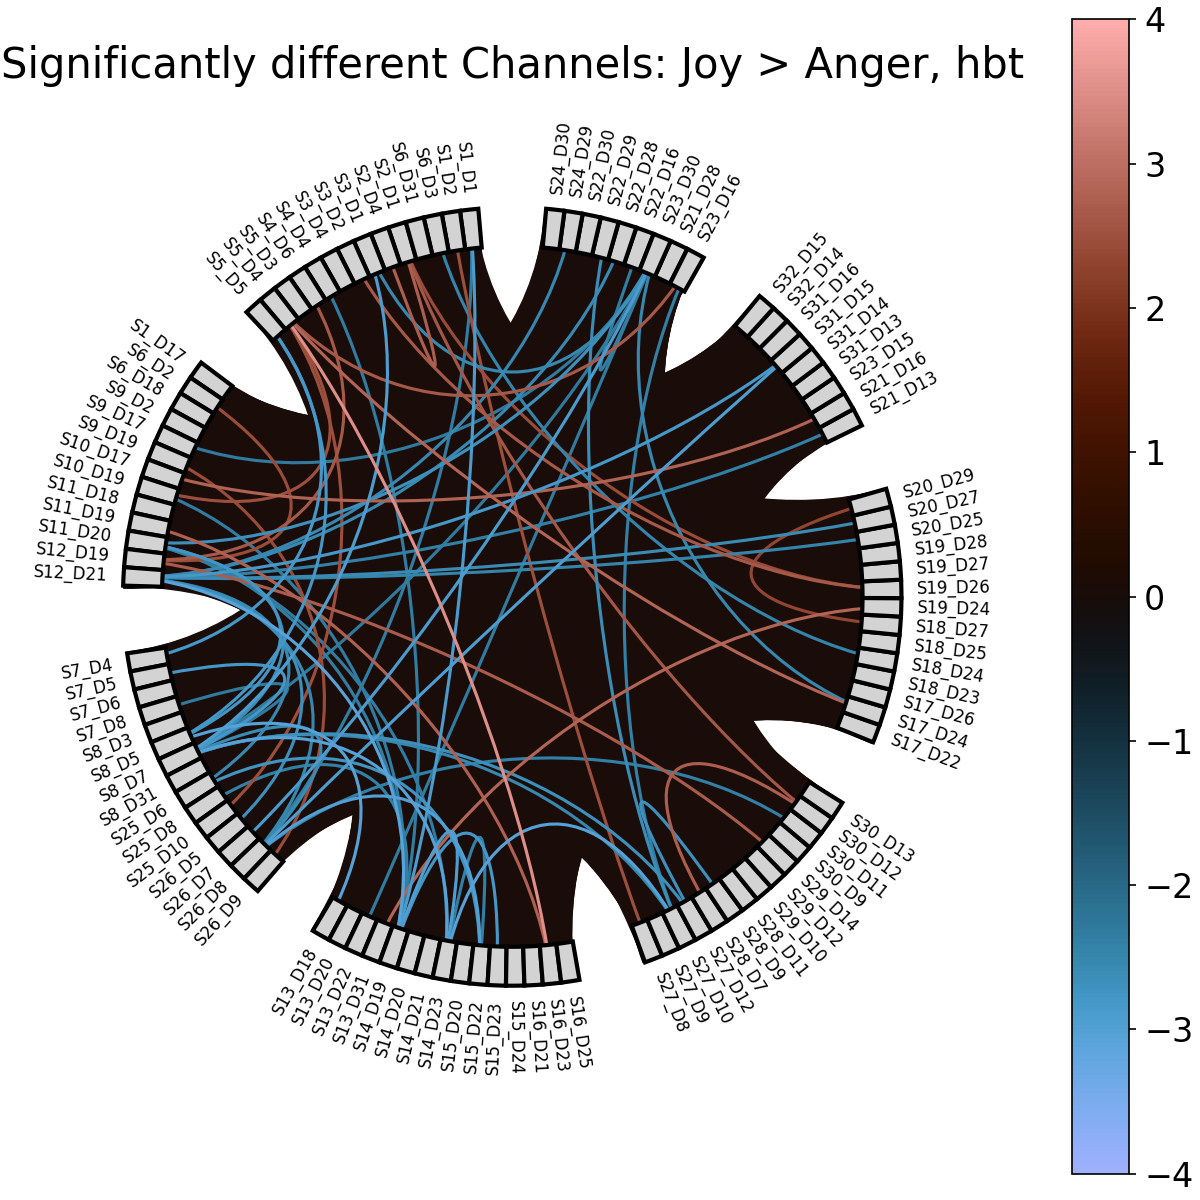
\includegraphics[width=0.24\textwidth]{C:/Users/super/OneDrive - Ontario Tech University/fNIRS_Emotions/plots/spectral_connectivity_time/chord_plots/group_level_t_tests_roi/emotion_Joy_Anger.png}
  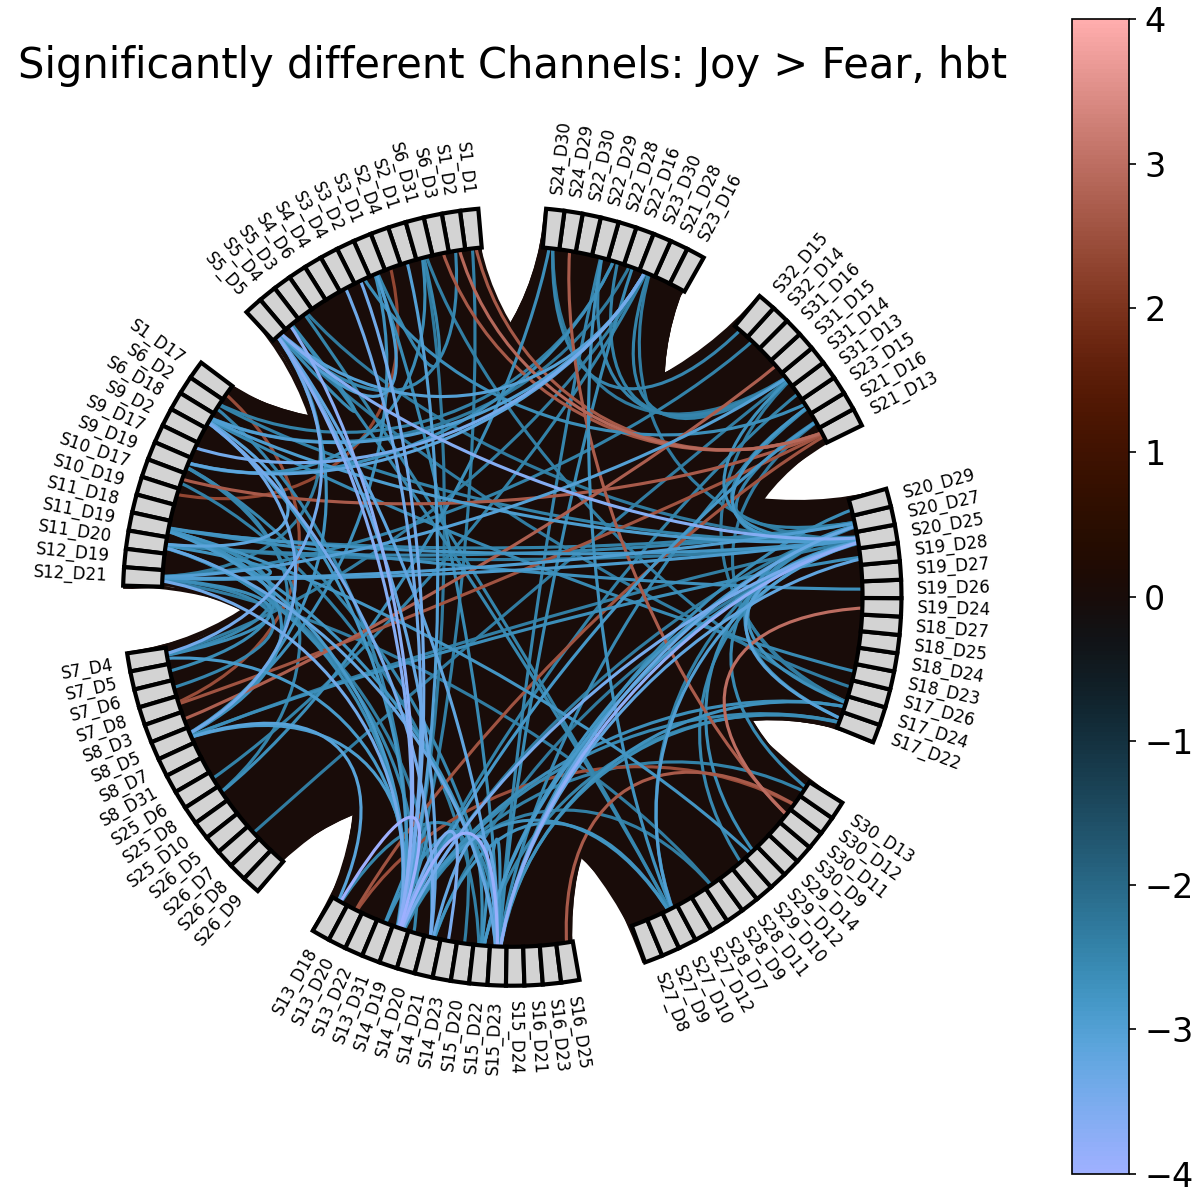
\includegraphics[width=0.24\textwidth]{C:/Users/super/OneDrive - Ontario Tech University/fNIRS_Emotions/plots/spectral_connectivity_time/chord_plots/group_level_t_tests_roi/emotion_Joy_Fear.png}
  \caption[FC: Emotion Contrasts (Fear and Anger)]{Functional connectivity results for Fear and Anger vs. the other emotions.
  Same concept as explained in figure \ref{fig:fc_real_vs_virtual}. }
  \label{fig:fc_emotion_analysis}
\end{figure}

The emotion contrasts (as shown in \ref{fig:fc_emotion_analysis}) revealed significant differences in functional connectivity across different emotions and ROI's.
The $t$-values show that Anger and Fear showed higher connectivity in general compared to the other emotions, and when compared to each other, Fear has only slightly higher connectivity than Anger. 
This higher connectivity for Anger and Fear as compared to the other emotions is consistent across most ROI's as well. 
The rest of the emotion contrasts can be found in Appendix \ref{tab:appendix_fc_emotion_analysis}, which shows the remaining set of contrasts for all emotions.

\begin{figure}[H]
  \centering
  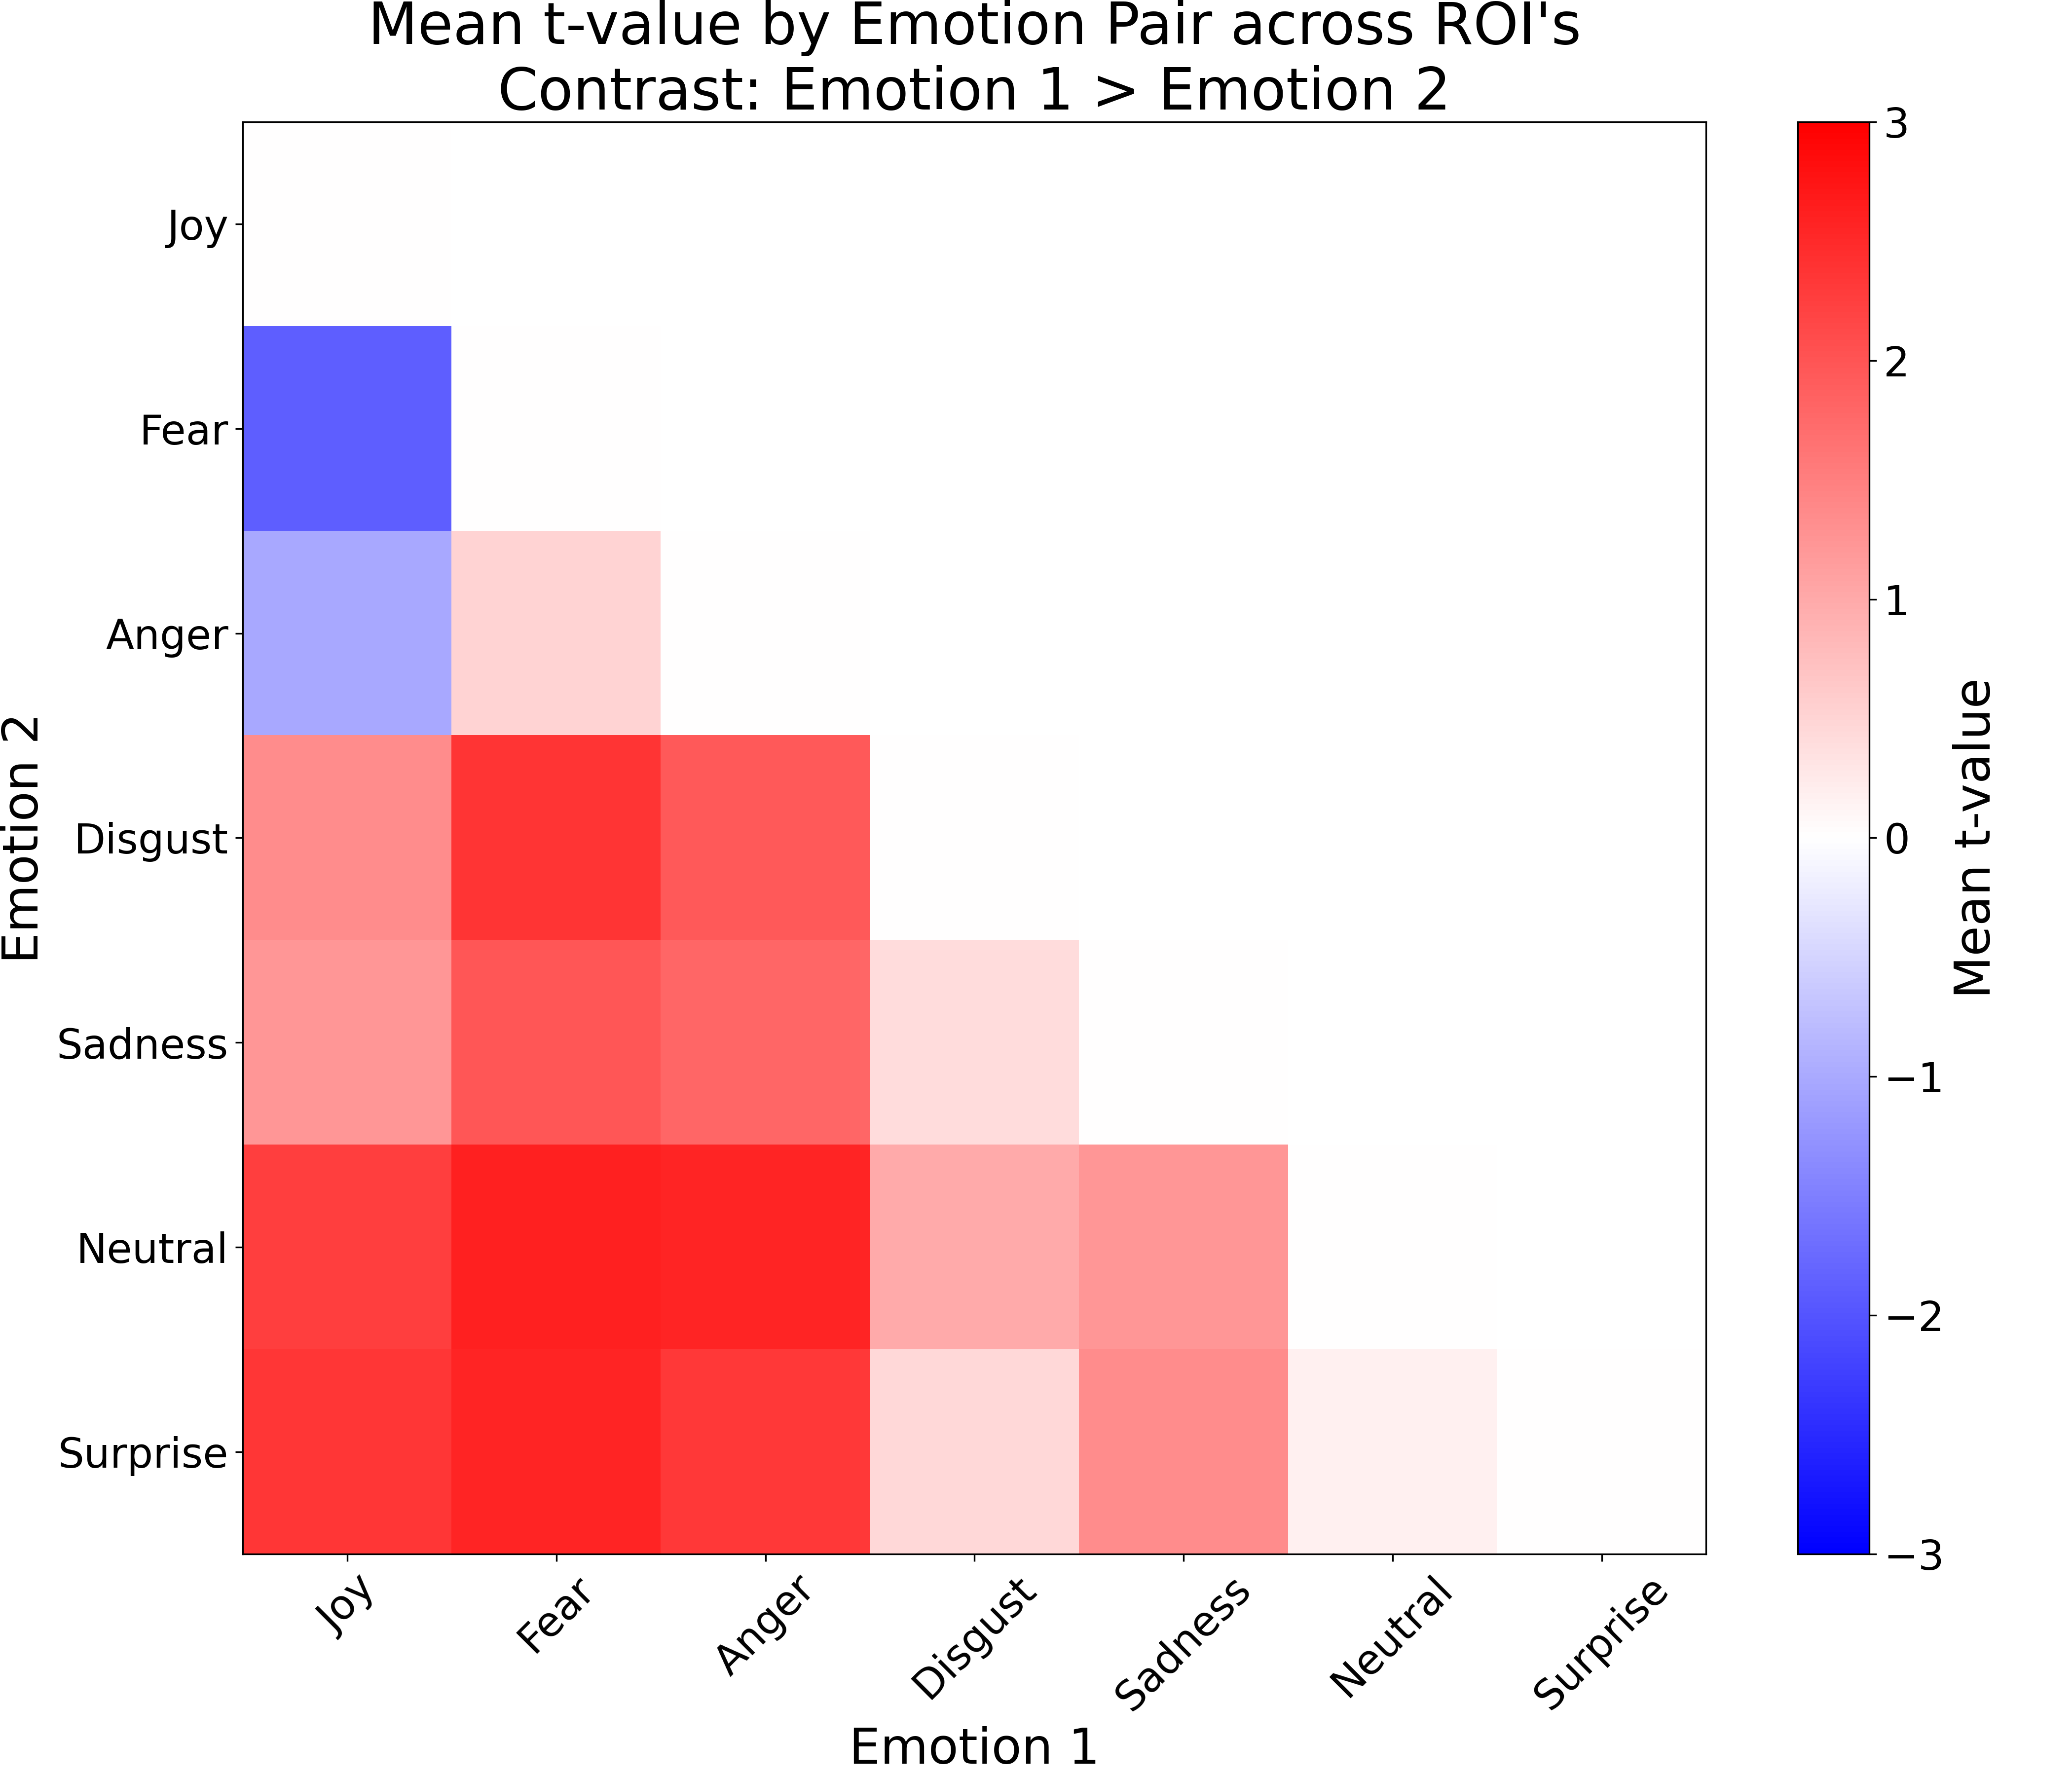
\includegraphics[width=1\textwidth]{C:/Users/super/OneDrive - Ontario Tech University/fNIRS_Emotions/plots/spectral_connectivity_time/emotion_analysis/Mean_t-value_by_Emotion_Pair.png}
  \caption[FC: Summary of Contrasts by Emotion Pair]{A heatmap summary of the functional connectivity results for the contrasts between different emotions.
  Red signifies that emotion 1 has higher connectivity than emotion 2, while blue signifies that emotion 2 has higher connectivity than emotion 1.
  The color bar on the right shows the $t$-value averaged across all significant channel pairs and across all ROI's, which indicates the strength of the difference in connectivity between the two emotions.
  This is the same value that is shown at the top of each plot in figure \ref{fig:fc_real_vs_virtual} and \ref{fig:fc_emotion_analysis}.}
  \label{fig:fc_emotion_summary_analysis}
\end{figure}

This summary of the functional connectivity results for the contrasts between different emotions (as shown in \ref{fig:fc_emotion_summary_analysis}) shows that Anger and Fear have the highest connectivity compared to the other emotions, with Fear having slightly higher connectivity than Anger.
This lines up with figure \ref{fig:fc_emotion_analysis}, which shows that Anger and Fear have higher connectivity compared to the other emotions.

\begin{figure}[H]
  \centering
  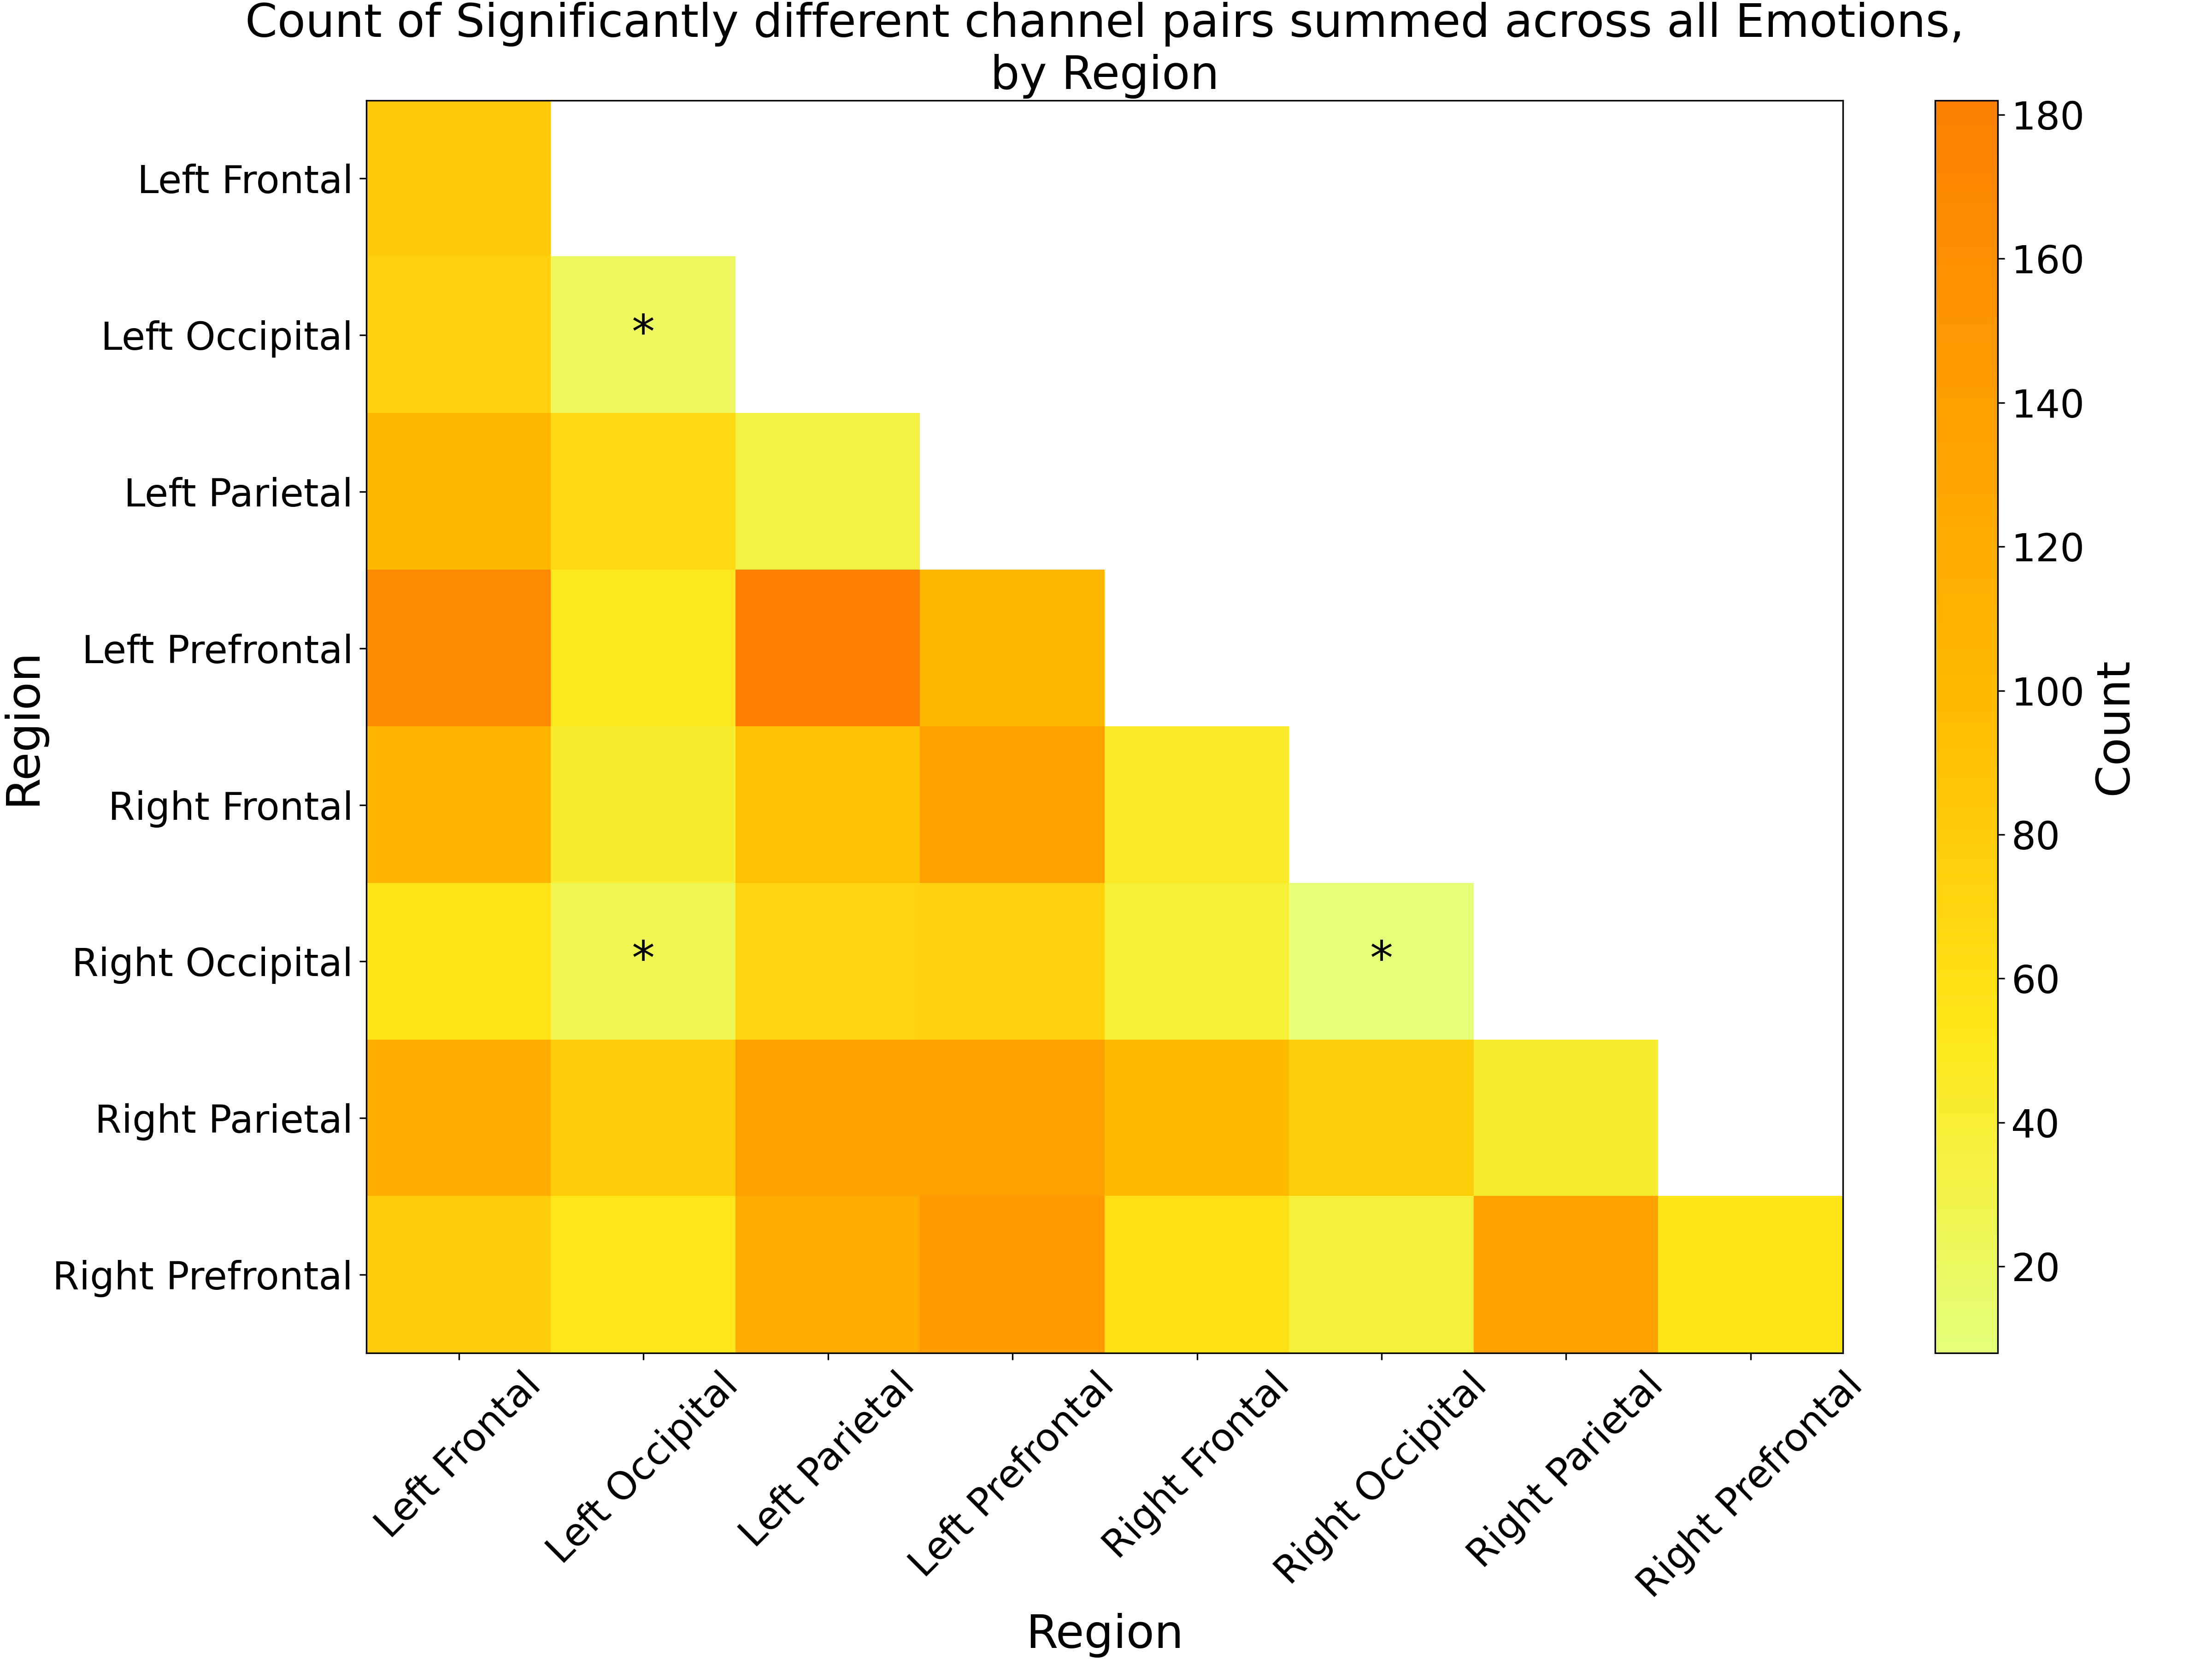
\includegraphics[width=1\textwidth]{C:/Users/super/OneDrive - Ontario Tech University/fNIRS_Emotions/plots/spectral_connectivity_time/emotion_analysis/Count_of_Significant_Channel_Pairs_by_Region.png}
  \caption[FC: Count of Significantly Different Channel Pairs by ROI]{A heatmap summary of the number of significantly different channel pairs for each ROI summed across all emotions. 
  The color bar on the right shows the number of significant channel pairs for each ROI, with brighter colors indicating a smaller number of significant channel pairs, and darker colors indicating a larger number of significant channel pairs.
  An asterisk was placed on the 3 ROI's with the least number of significantly different channel pairs to indicate that these ROI's are more synchronized with each other than any other pair of ROI's, regardless of the emotion.
  Note that ROI's can have differences within them, as each ROI is made up of multiple channels, and the differences are calculated between channels within the same ROI.}
  \label{fig:fc_region_summary_analysis}
\end{figure}

The count of significantly different channel pairs for each ROI summed across all emotions (as shown in \ref{fig:fc_region_summary_analysis}) marks 3 regions with an asterisk, these regions have less channel pairs that are significantly different from each other, meaning that these regions are more synchronized with each other than any other pair of ROI's.
These regions are the left occipital/right occipital, left occipital/left occipital, and right occipital/right occipital ROI's.
This indicates that the differences in processing emotions occur in the frontal, prefrontal, and parietal regions of the brain.

\subsection{Face Type \texorpdfstring{$\times$}{x} Emotion Contrasts}
\begin{figure}[H]
  \centering
  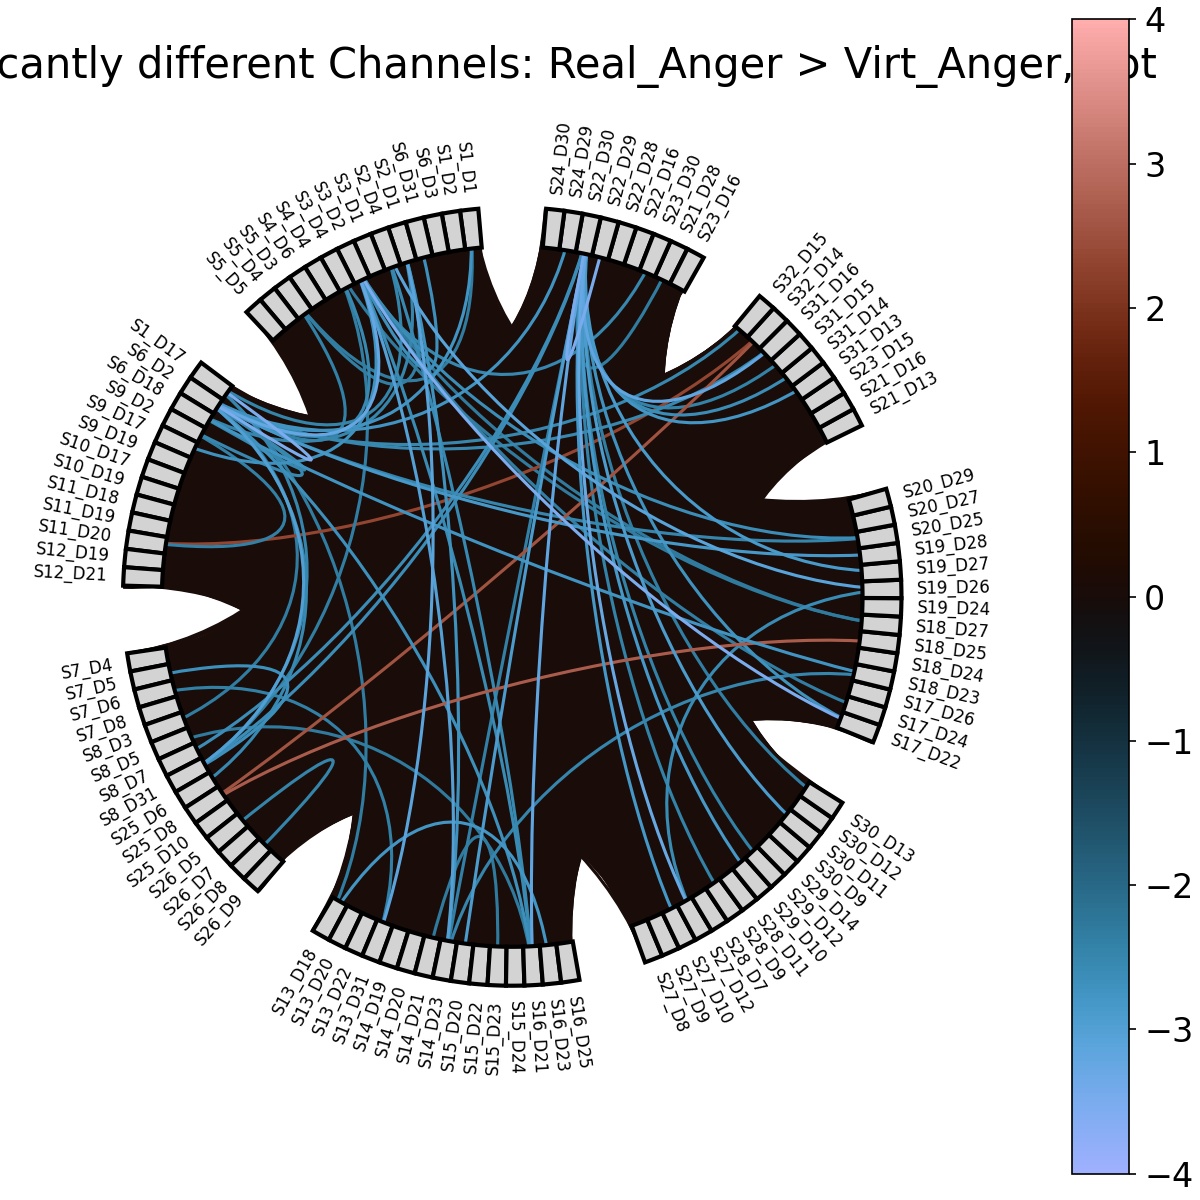
\includegraphics[width=0.3\textwidth]{C:/Users/super/OneDrive - Ontario Tech University/fNIRS_Emotions/plots/spectral_connectivity_time/chord_plots/group_level_t_tests_roi/face_type_emotion_Real_Anger_Virt_Anger.png}
  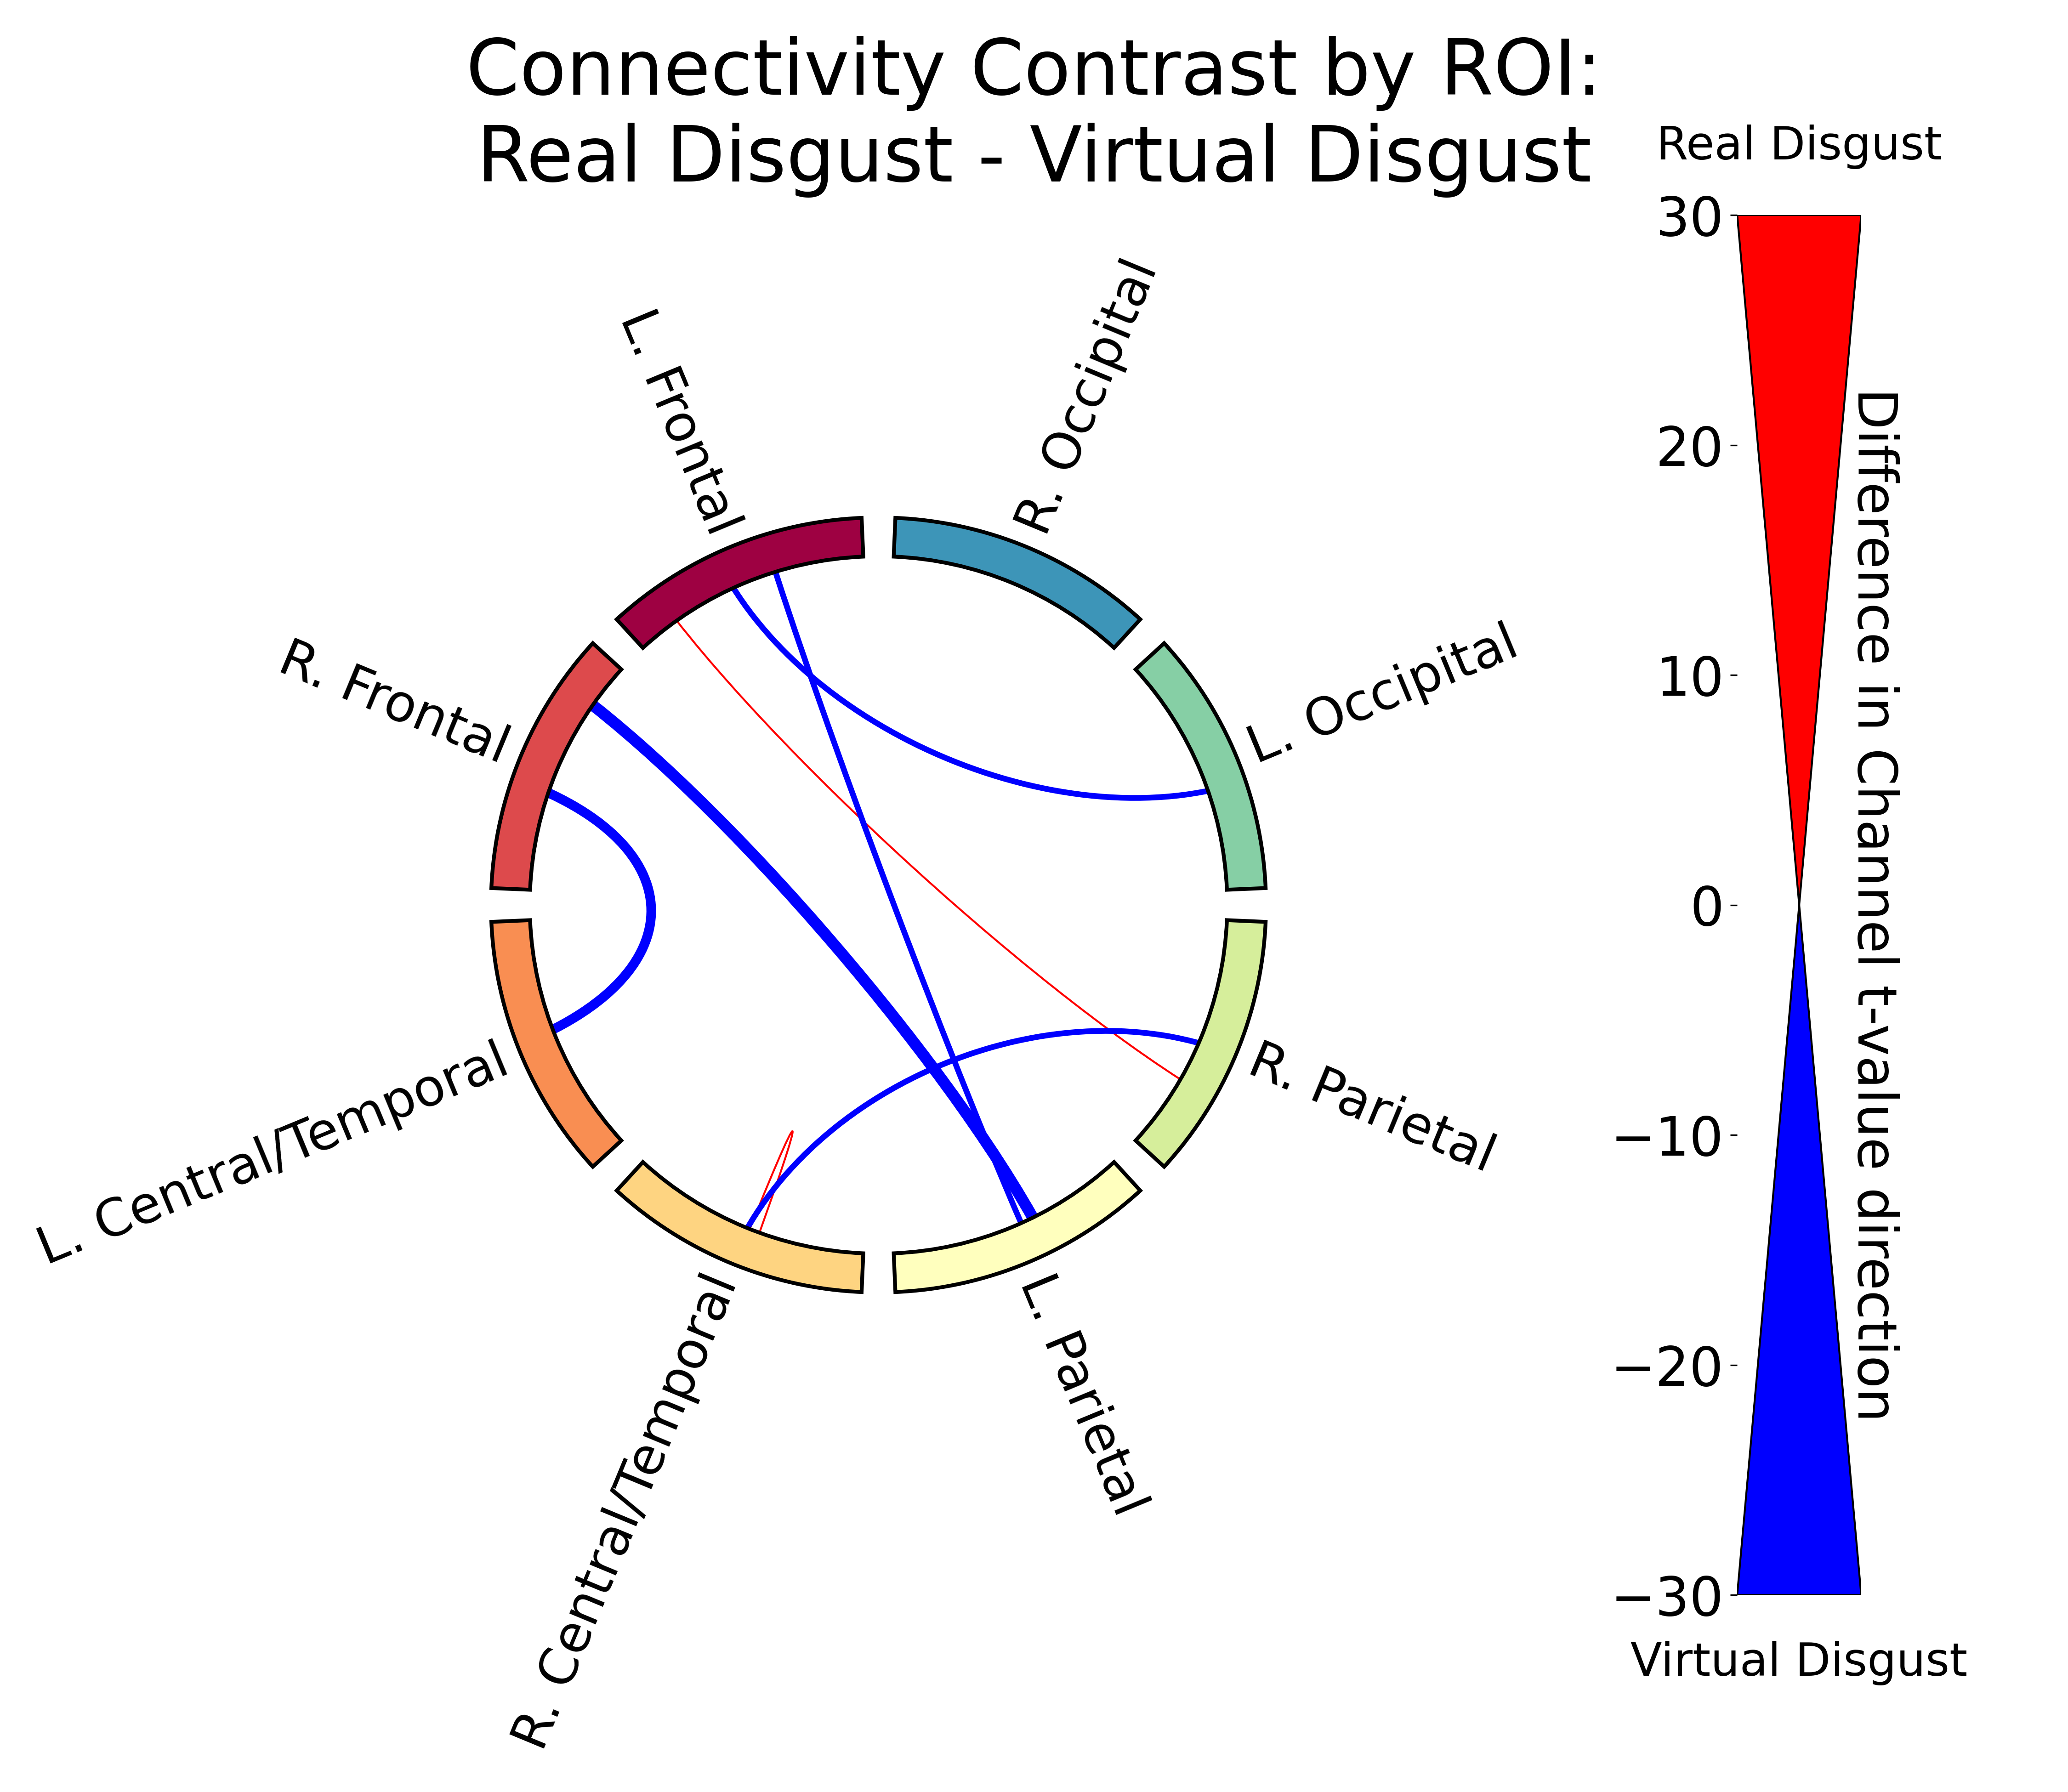
\includegraphics[width=0.3\textwidth]{C:/Users/super/OneDrive - Ontario Tech University/fNIRS_Emotions/plots/spectral_connectivity_time/chord_plots/group_level_t_tests_roi/face_type_emotion_Real_Disgust_Virt_Disgust.png}
  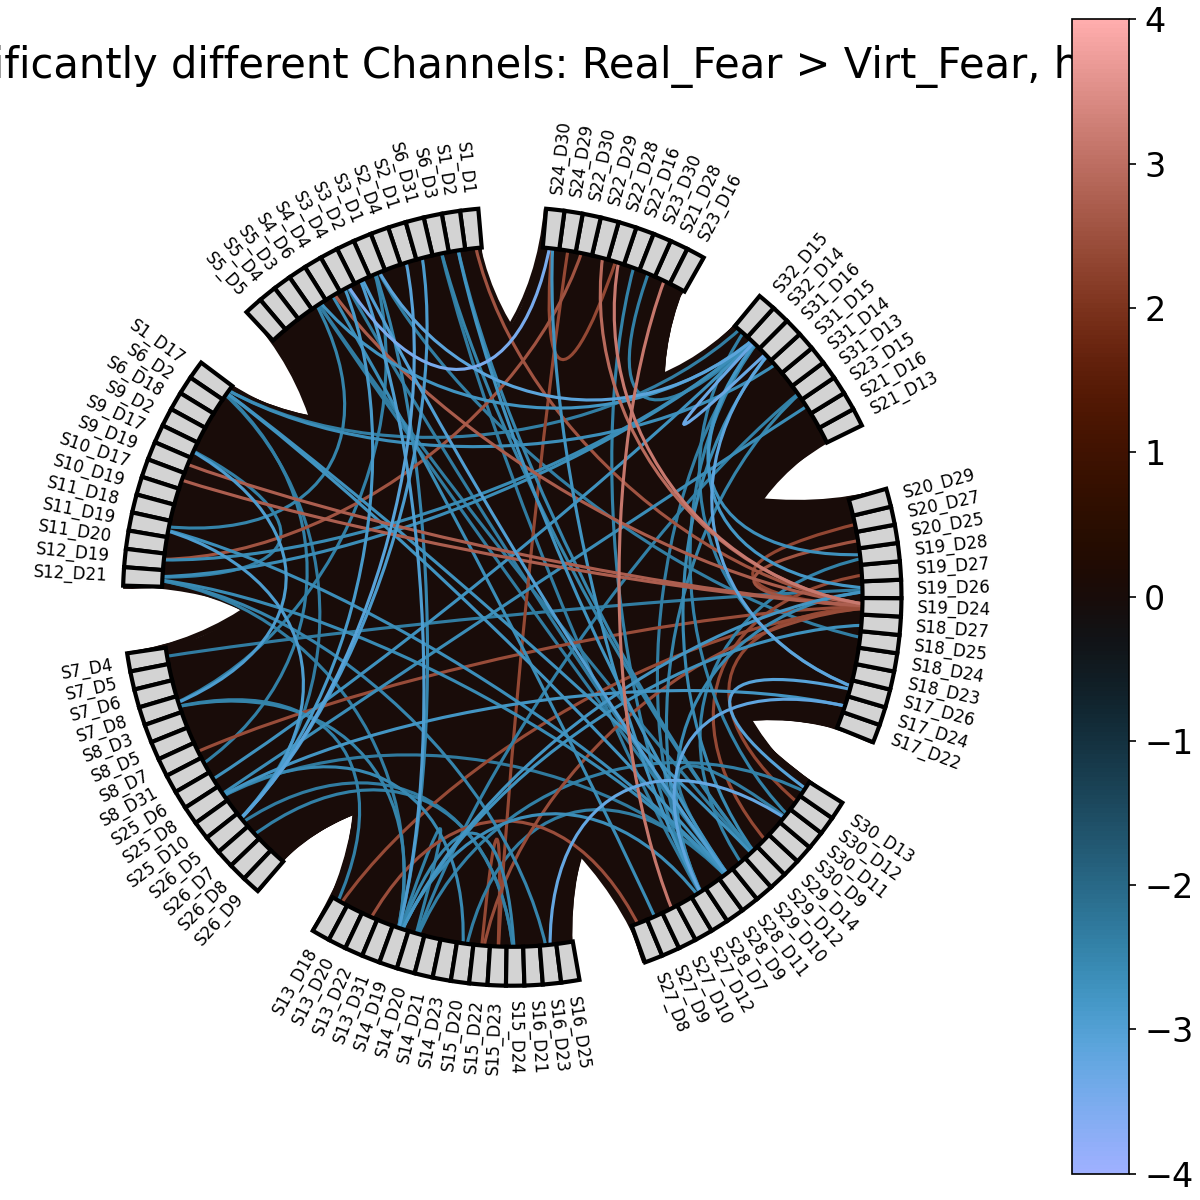
\includegraphics[width=0.3\textwidth]{C:/Users/super/OneDrive - Ontario Tech University/fNIRS_Emotions/plots/spectral_connectivity_time/chord_plots/group_level_t_tests_roi/face_type_emotion_Real_Fear_Virt_Fear.png}
  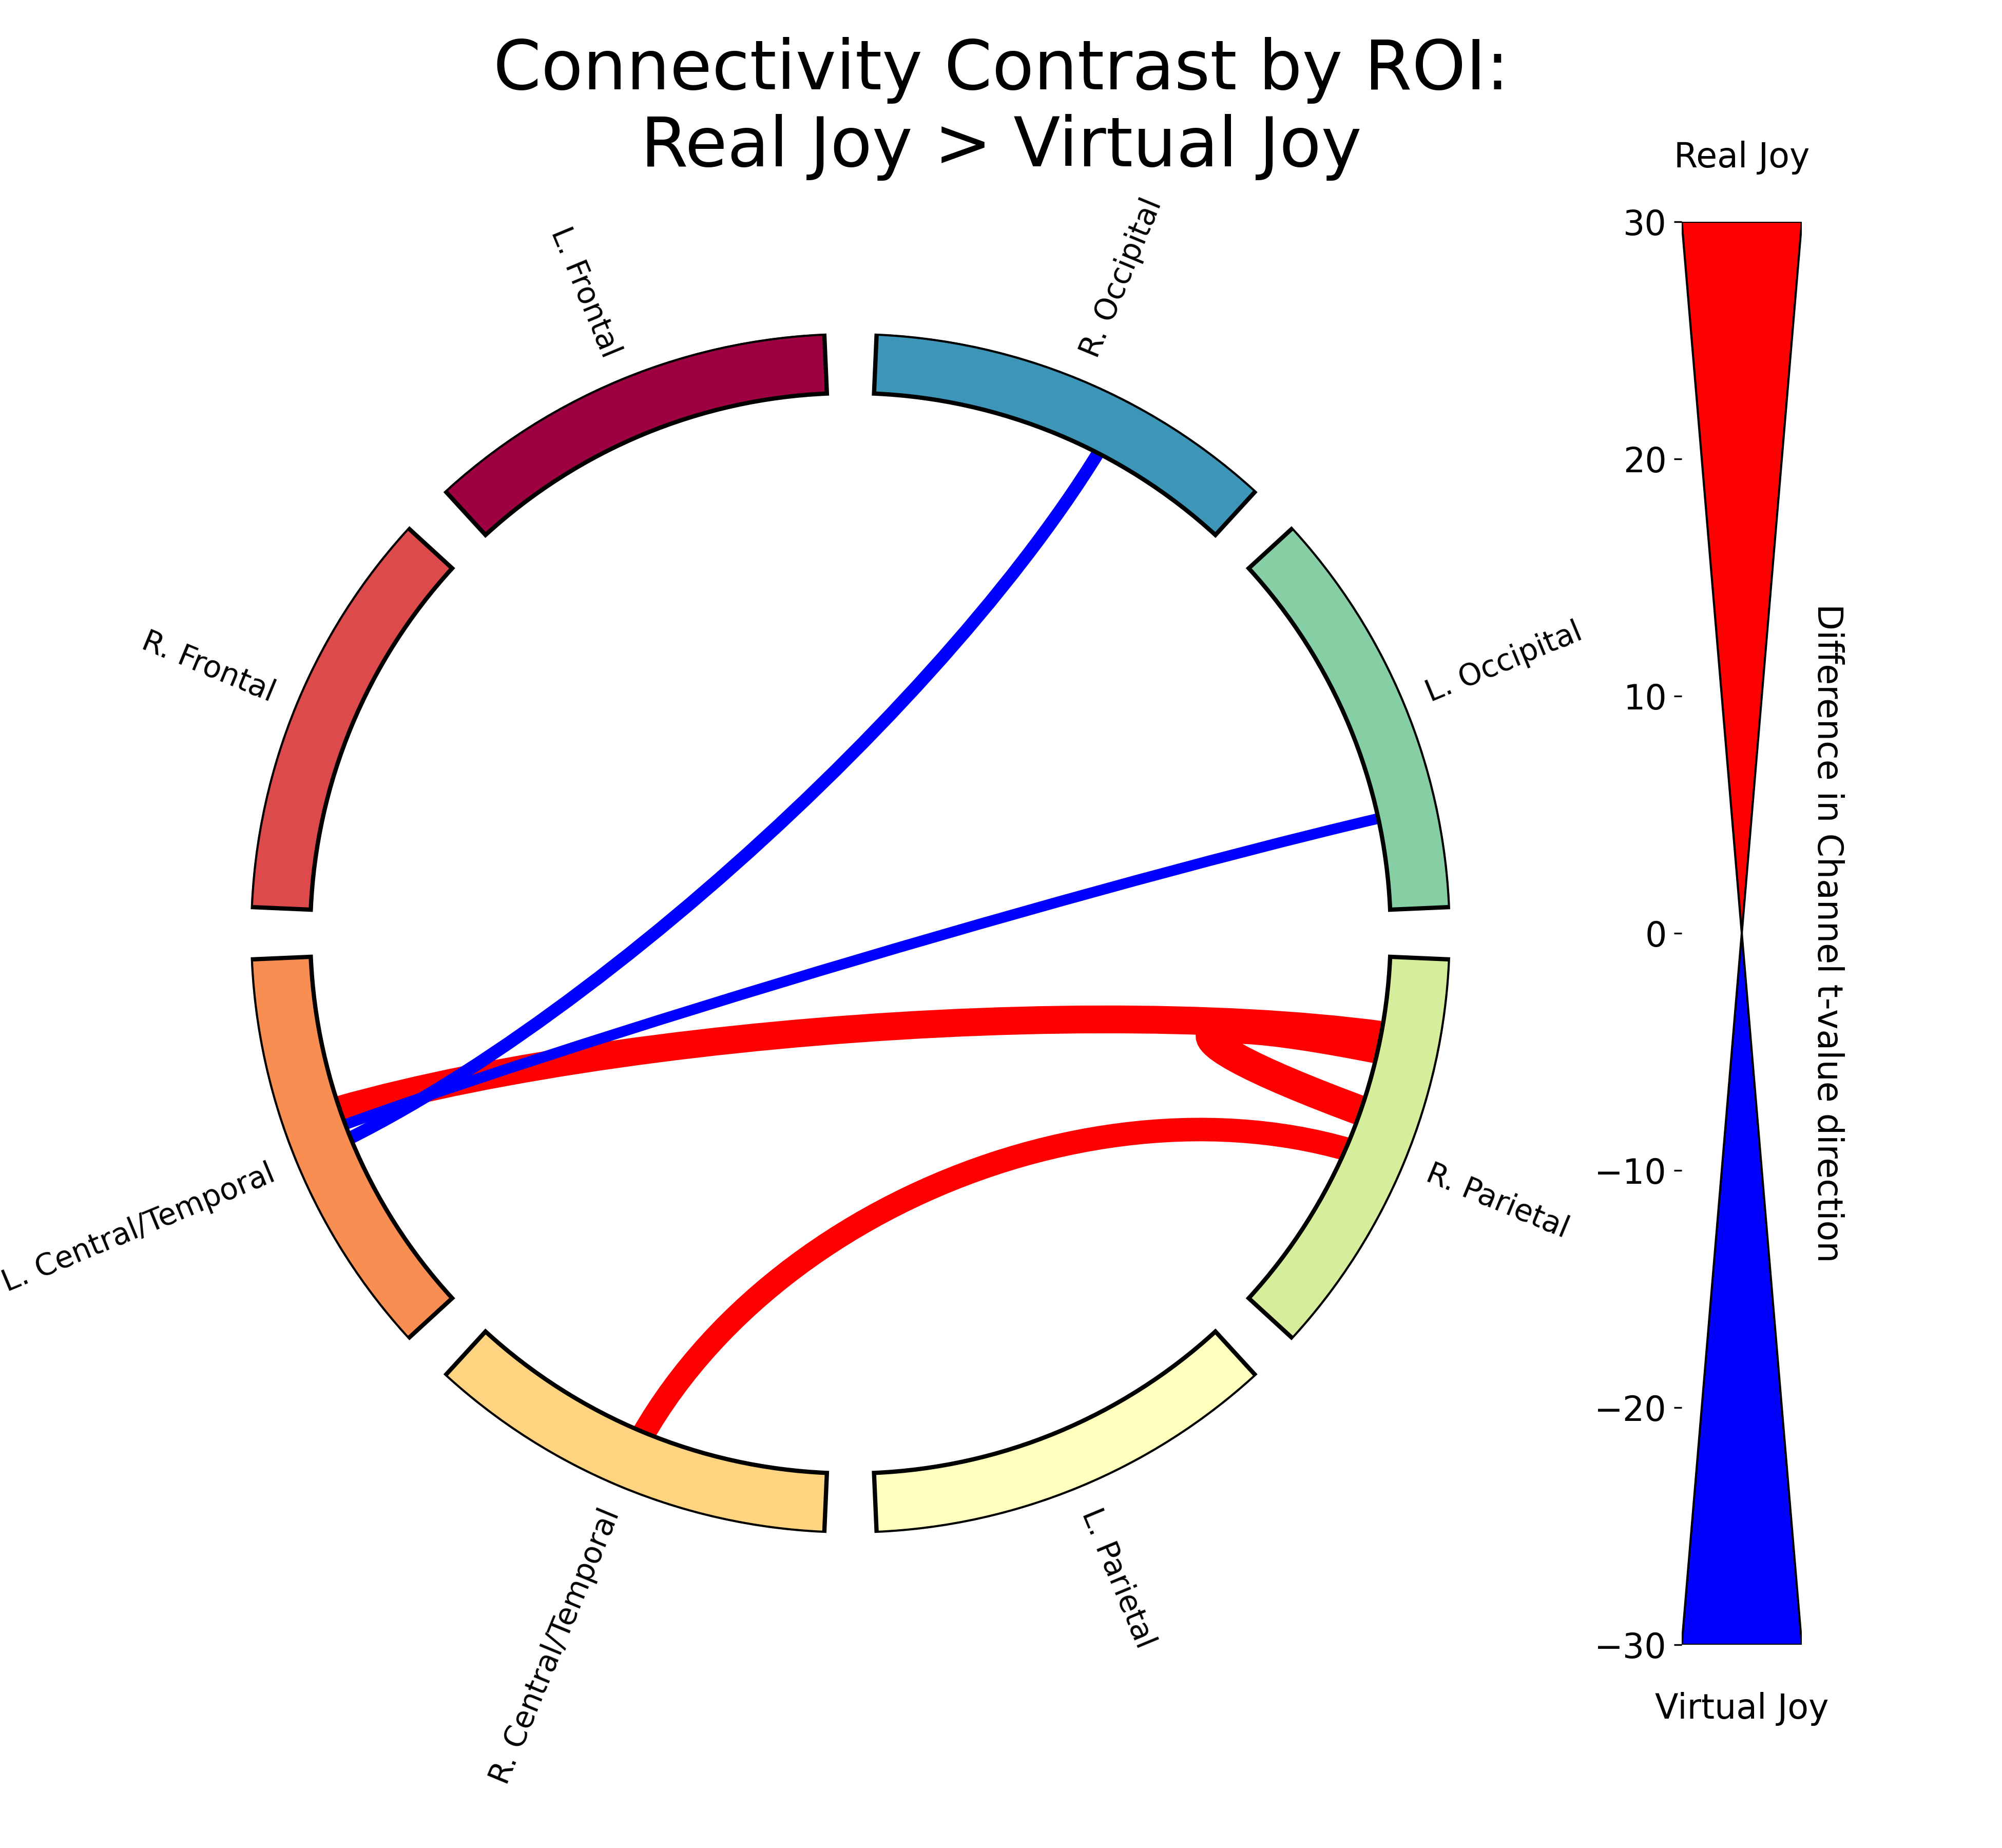
\includegraphics[width=0.3\textwidth]{C:/Users/super/OneDrive - Ontario Tech University/fNIRS_Emotions/plots/spectral_connectivity_time/chord_plots/group_level_t_tests_roi/face_type_emotion_Real_Joy_Virt_Joy.png}
  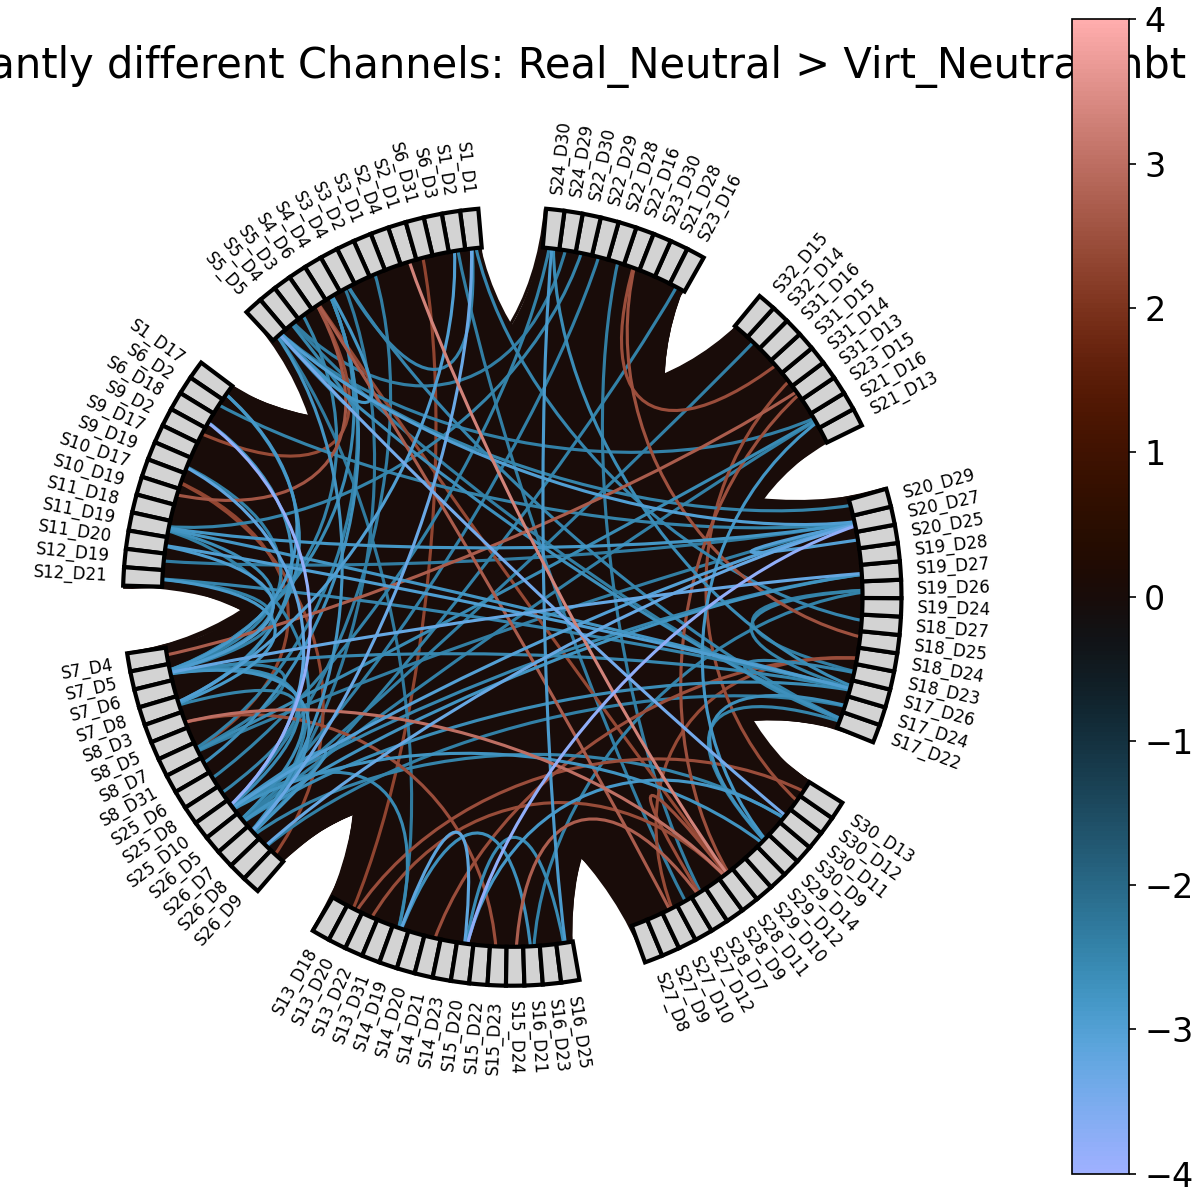
\includegraphics[width=0.3\textwidth]{C:/Users/super/OneDrive - Ontario Tech University/fNIRS_Emotions/plots/spectral_connectivity_time/chord_plots/group_level_t_tests_roi/face_type_emotion_Real_Neutral_Virt_Neutral.png}
  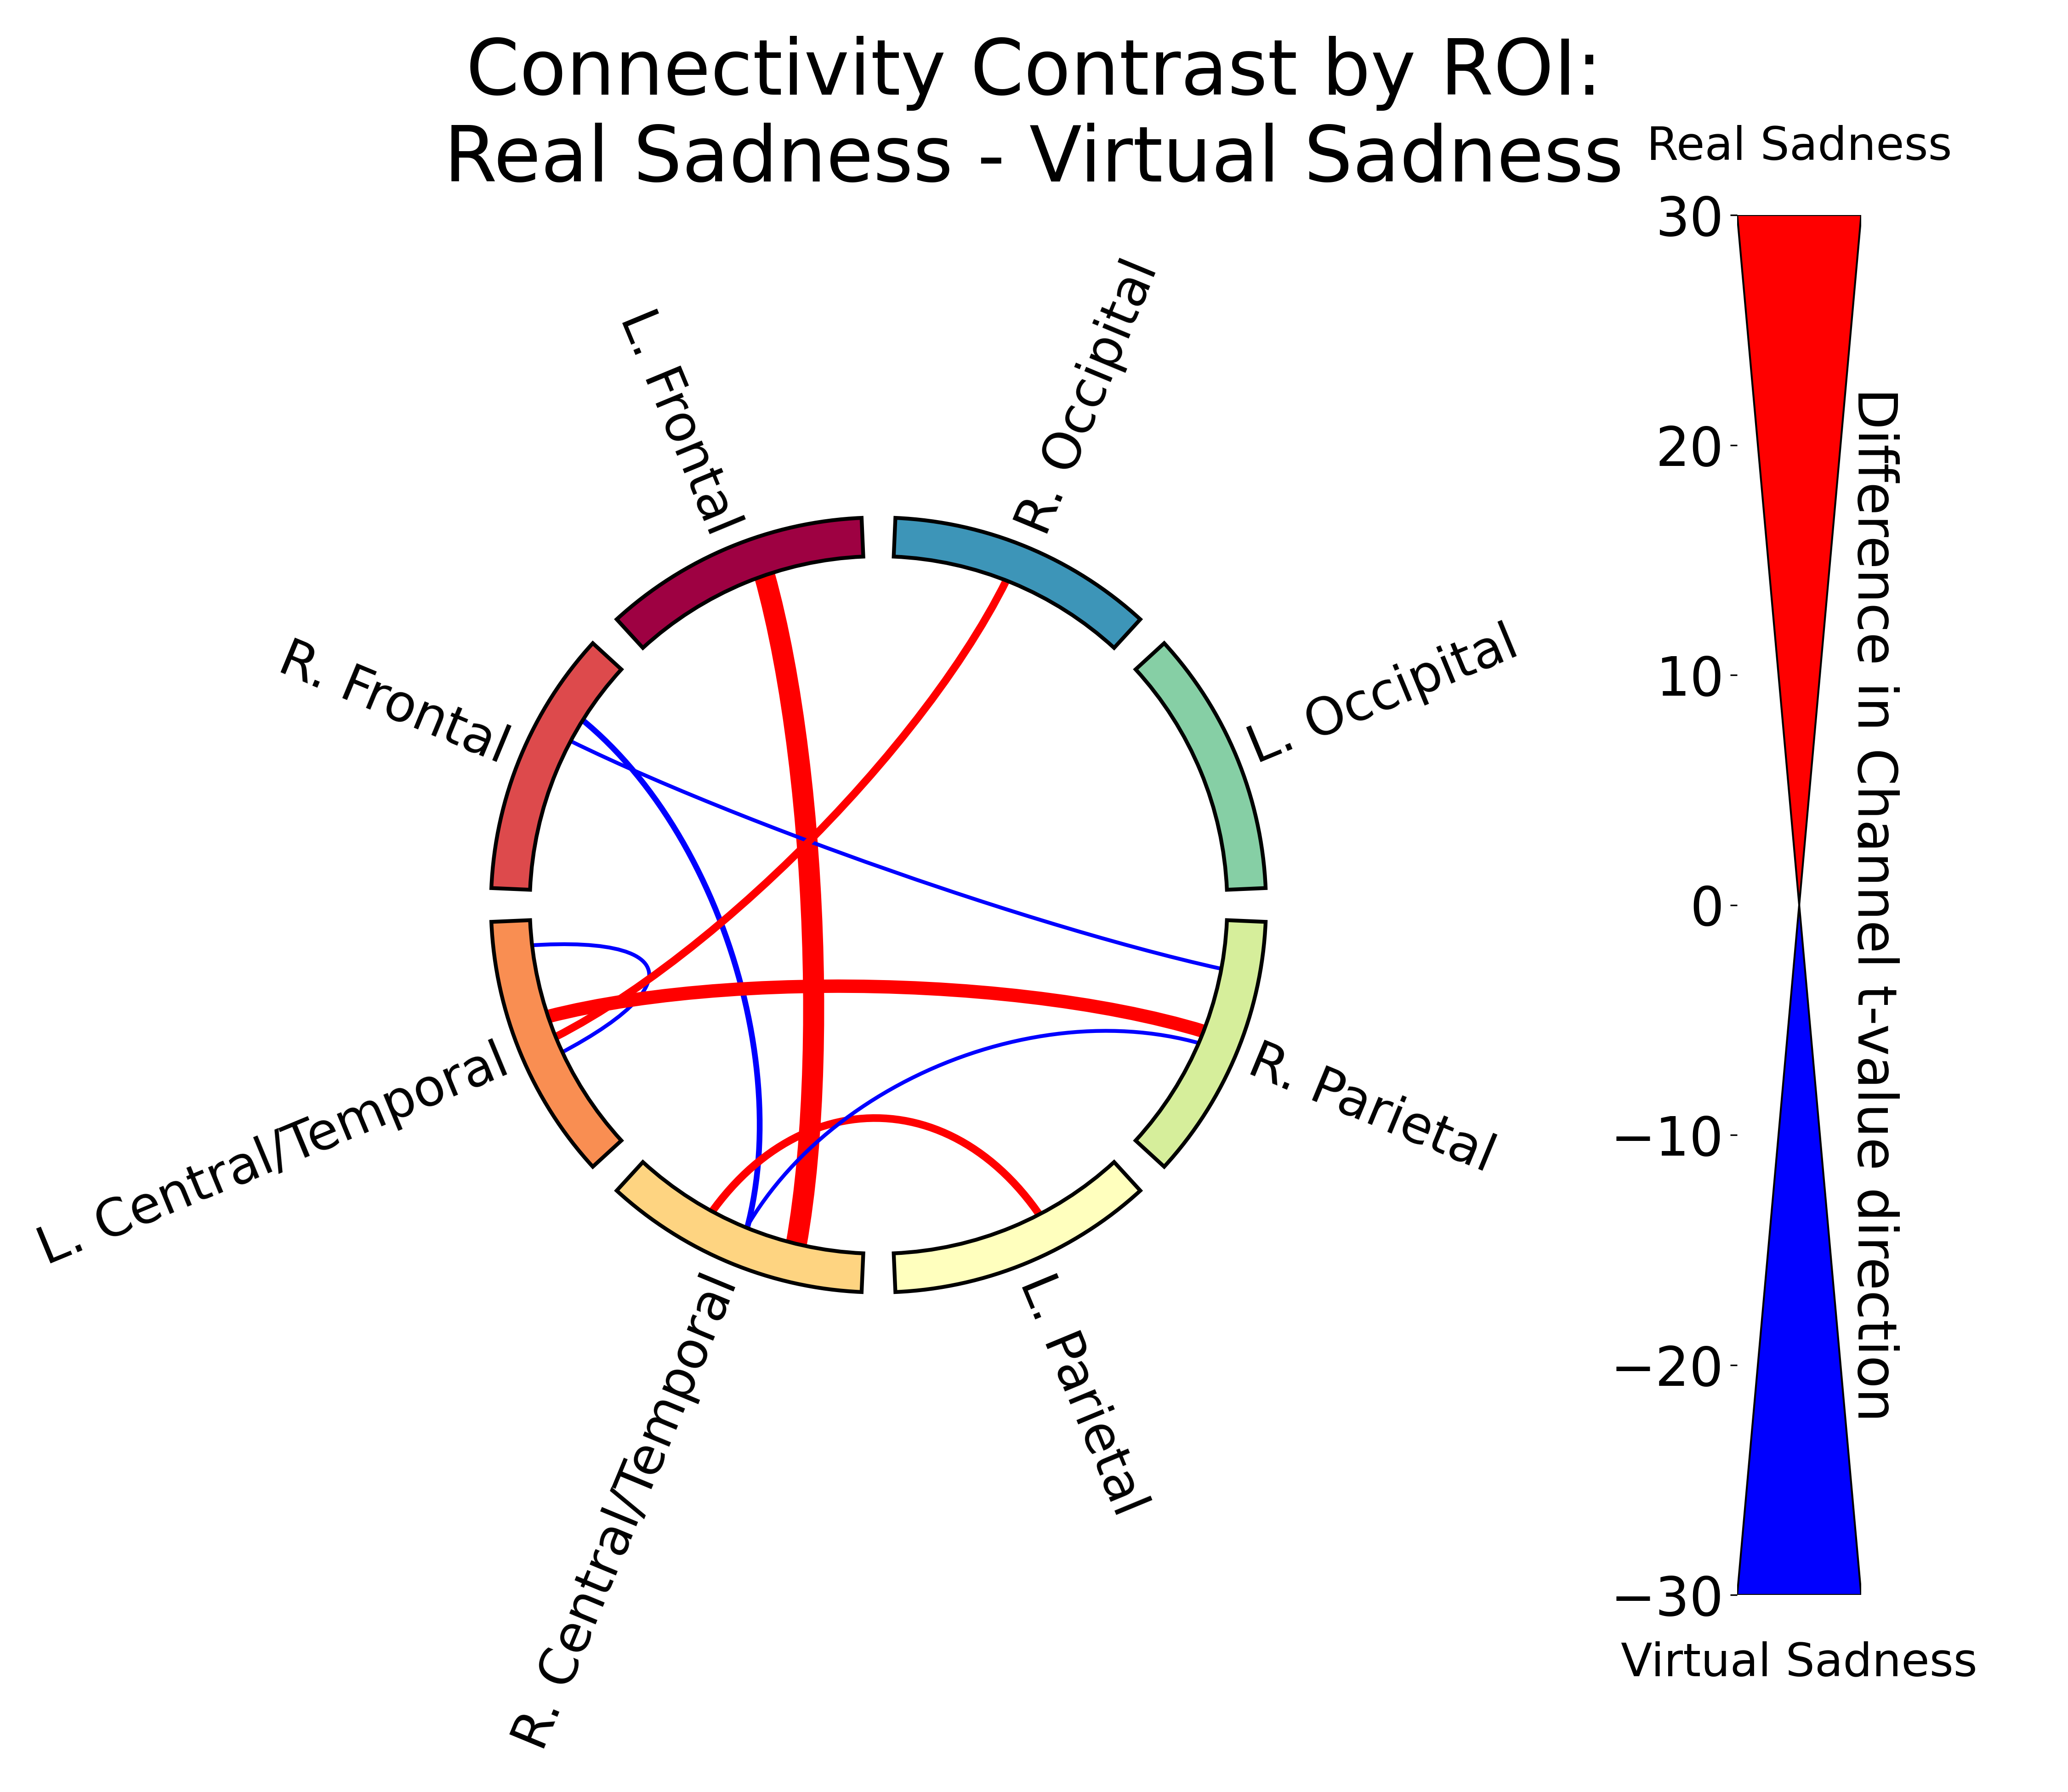
\includegraphics[width=0.3\textwidth]{C:/Users/super/OneDrive - Ontario Tech University/fNIRS_Emotions/plots/spectral_connectivity_time/chord_plots/group_level_t_tests_roi/face_type_emotion_Real_Sadness_Virt_Sadness.png}
  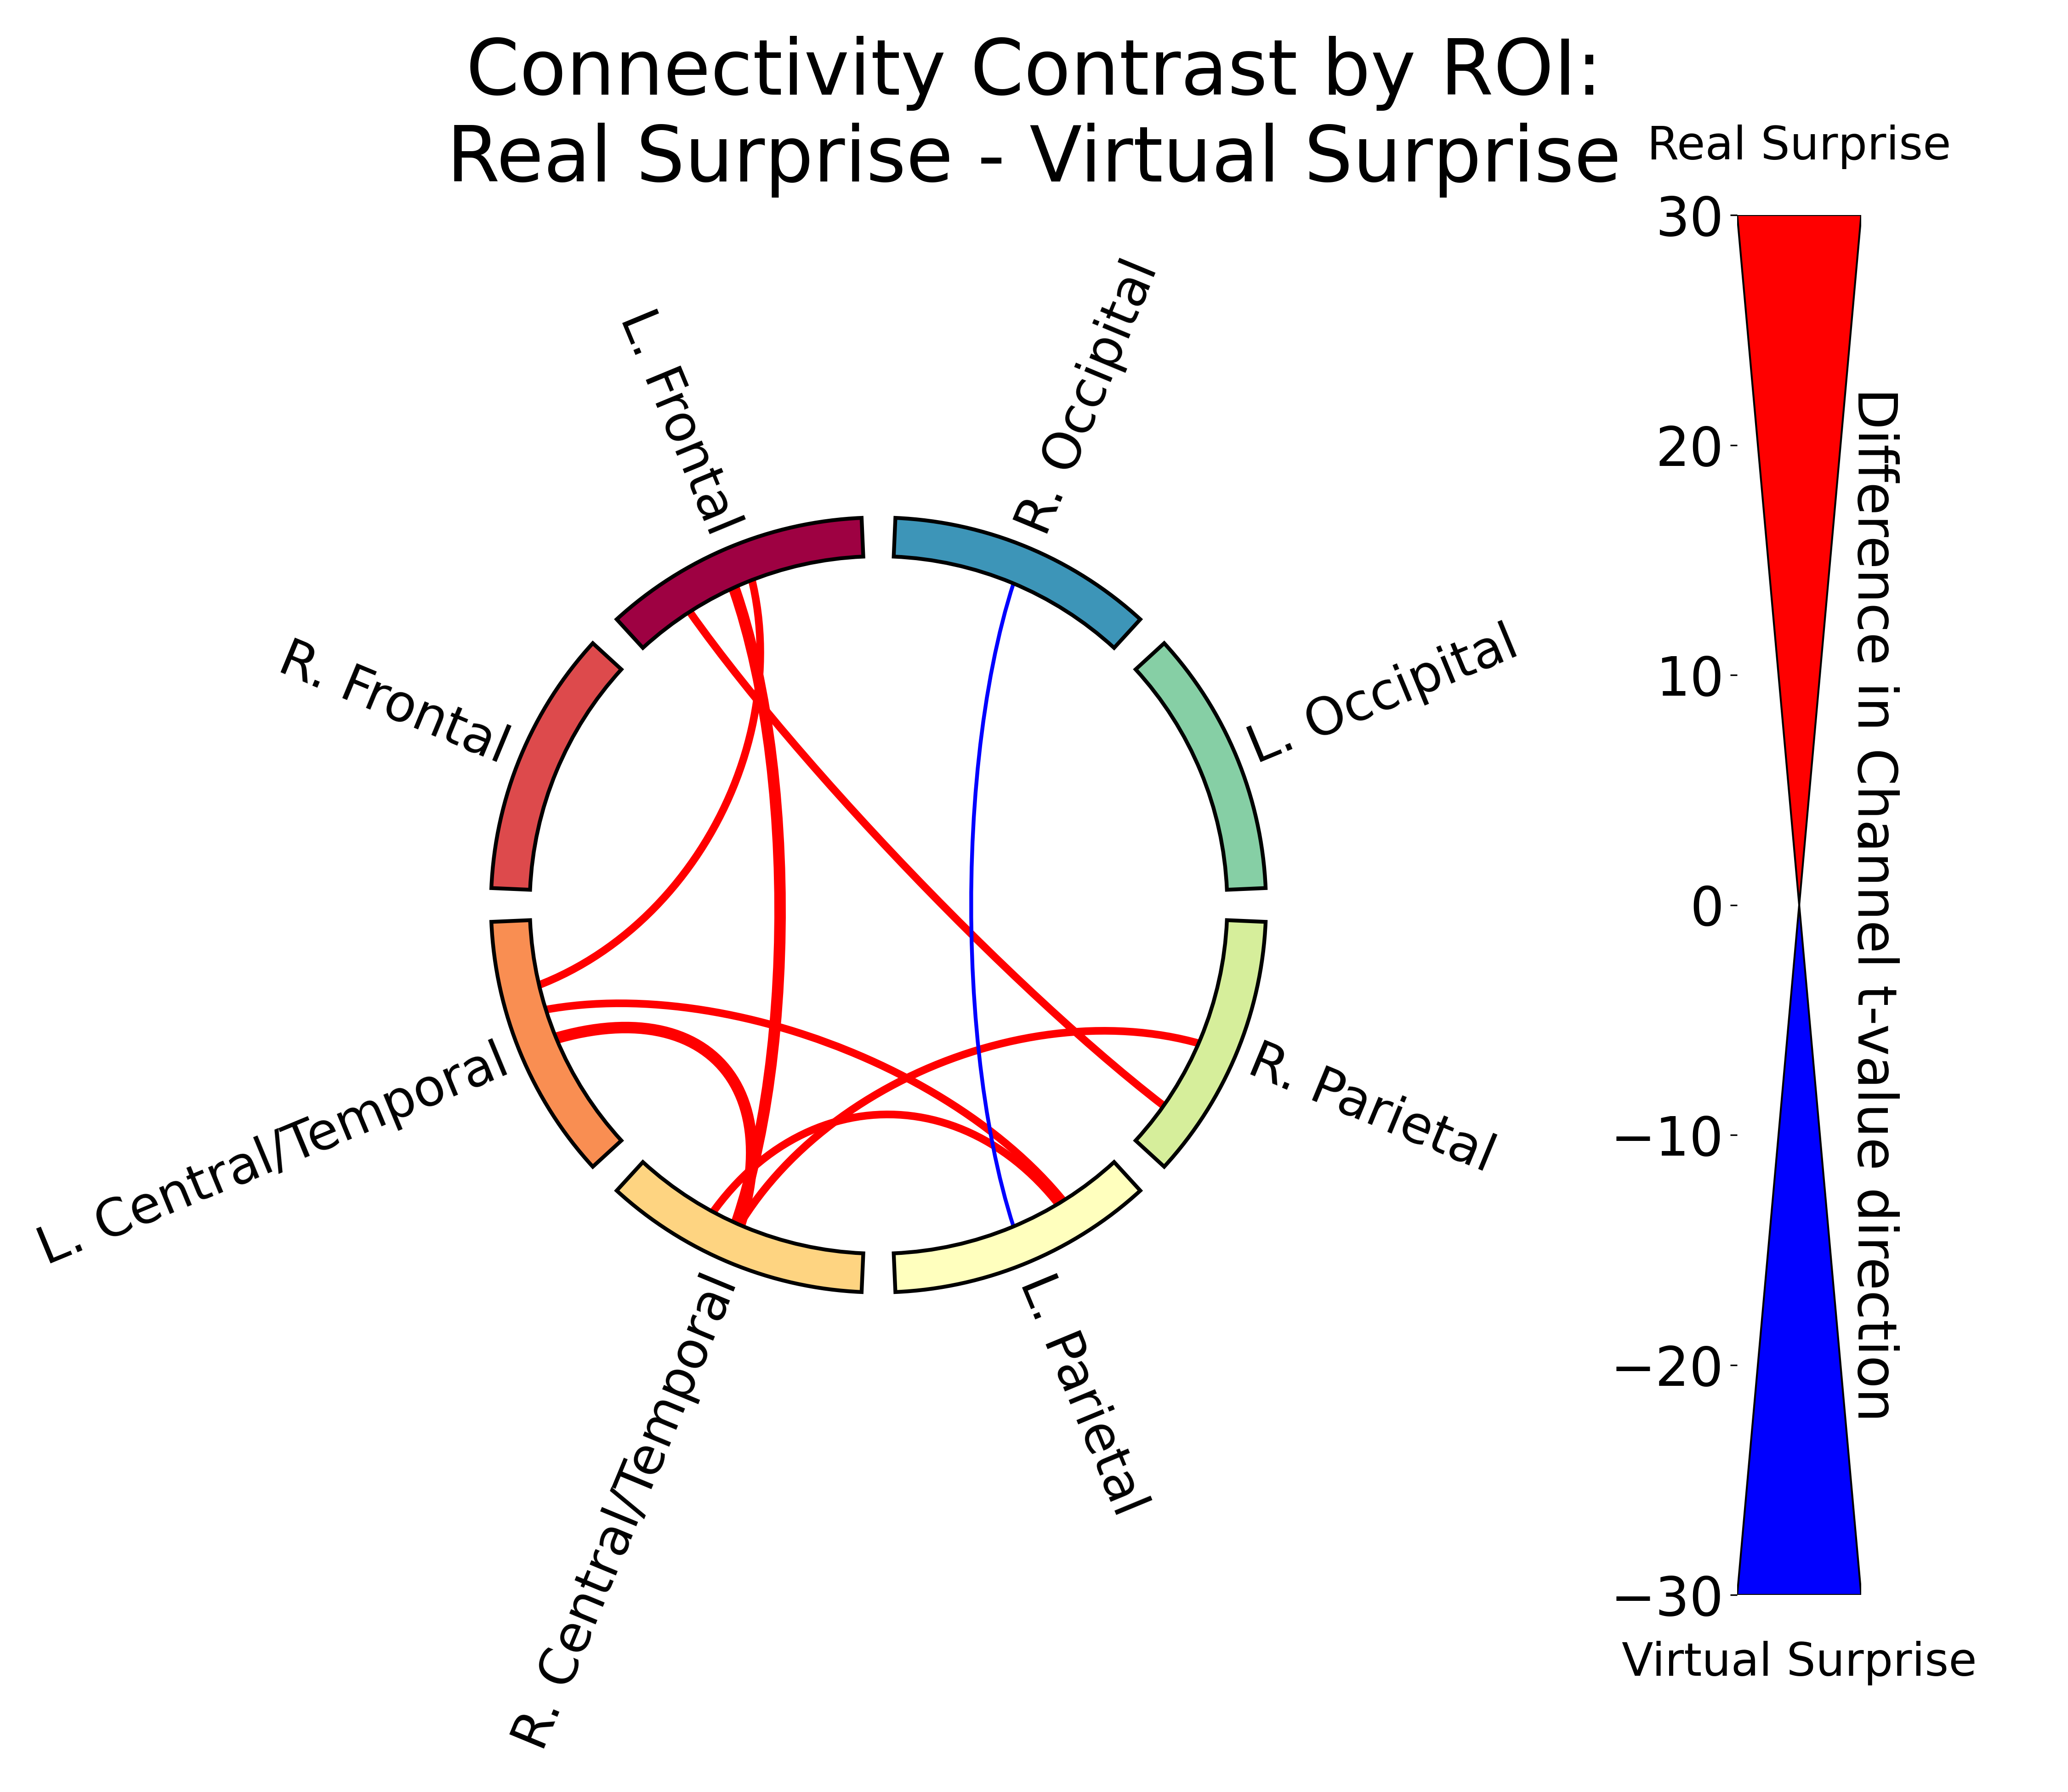
\includegraphics[width=0.3\textwidth]{C:/Users/super/OneDrive - Ontario Tech University/fNIRS_Emotions/plots/spectral_connectivity_time/chord_plots/group_level_t_tests_roi/face_type_emotion_Real_Surprise_Virt_Surprise.png}
  \caption[FC: Face Type \texorpdfstring{$\times$}{x} Emotion Contrasts]{Functional connectivity results for the contrast between real and virtual conditions within each emotion.
  Same concept as explained in figure \ref{fig:fc_real_vs_virtual}. }
  \label{fig:fc_real_vs_virtual_emotion_analysis}
\end{figure}

The interaction of face type with emotion (Real $>$ Virt within each emotion as shown in \ref{fig:fc_real_vs_virtual_emotion_analysis}) revealed significant differences in functional connectivity across both face types within each emotion.
For Anger, Disgust, Fear, and Neutral, virtual faces showed higher connectivity across most ROI's compared to real faces, whereas for Joy, Sadness, and Surprise, real faces showed higher connectivity across most ROI's compared to virtual faces.
Like the GLM results, this indicates that the neural response to emotional expressions is modulated by the realism of the face stimuli, with different patterns of connectivity observed for each face type \texorpdfstring{$\times$}{x} emotion interaction.

The full table of the functional connectivity contrasts for all main effects and interactions can be found in Appendix \ref{tab:appendix_fc_emotion_analysis}.

\section{Memory Task Results}
\begin{figure}[H]
  \centering
  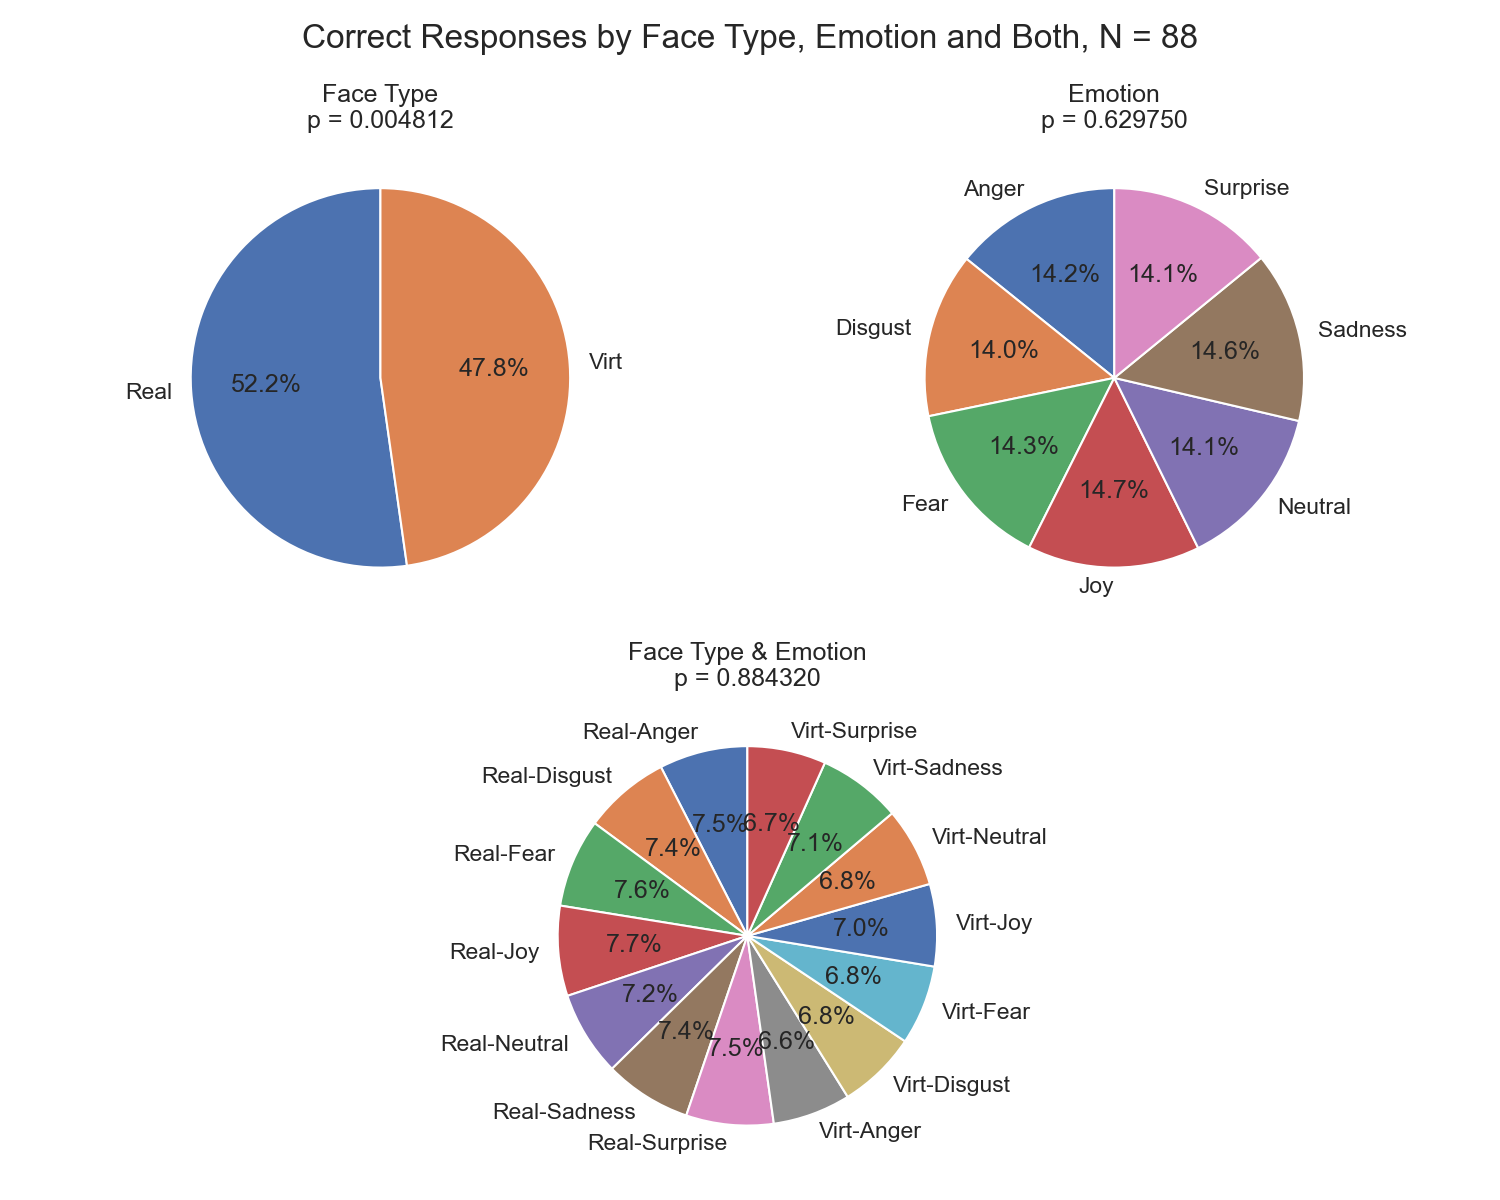
\includegraphics[width=0.9\textwidth]{C:/Users/super/OneDrive - Ontario Tech University/fNIRS_Emotions/plots/behavioural_responses/correct_responses_by_face_type_emotion.png}
  \caption[Correct Memory Task Responses by Face Type and Emotion]{Proportion correct by condition in the memory task, plotted separately for real and virtual faces, for each emotion, and the interaction between face type and emotion. 
  The $p$-values indicate the significance of the main effects and interaction. }
  \label{fig:memory_task_results}
\end{figure}

A two-way Type III ANOVA (as described in \ref{sec:memory_task_analysis}) was conducted to examine the main effects and interaction on memory performance (proportion correct). 
Figure \ref{fig:memory_task_results} shows accuracy by face type/emotion and their interaction.
The analysis revealed a significant main effect of face type, $F(1,4802)=7.96$, $p=0.0048$, indicating that memory performance was higher for real faces compared to virtual faces. 
There was no significant main effect of emotion, $F(6,4802)=0.83$, $p=0.55$, nor a significant interaction between face type and emotion, $F(6,4802)=0.46$, $p=0.84$. 
These findings suggest that while the realism of the face influences memory performance, the specific emotional expression does not have a significant impact on memory accuracy.
The full ANOVA table is shown in Appendix \ref{tab:appendix_memory_task_anova}.